\documentclass[UKenglish, aspectratio = 169]{beamer}

% theme and packages
\usetheme{Bear}
\usepackage{relsize}
\usepackage{pgfplots} 
\usepackage{movie15} 
\usepackage{pgf-pie}
\usepackage{csvsimple}
\usepackage{pdfpages}
\usepgfplotslibrary{
    groupplots,
    units
}

\usepackage{datetime}
\newdate{date}{05}{10}{2023}
\date{\displaydate{date}}

% doc setup
\author[Antonio Pucciarelli]{\href{https://github.com/antoniopucciarelli}{Antonio Pucciarelli}}
\title{\textsc{Machine Learning \\ for Turbomachinery}}
\subtitle{Data-Driven Design Methods for High-Speed Turbines}

\begin{document}
\hidelogo

\section{Overview}
\SectionPage

\begin{frame}{Overview}
    \only<1>{
        \begin{columns}
            \column{0.5\textwidth}
                \begin{figure}[H]
                    \centering 
                    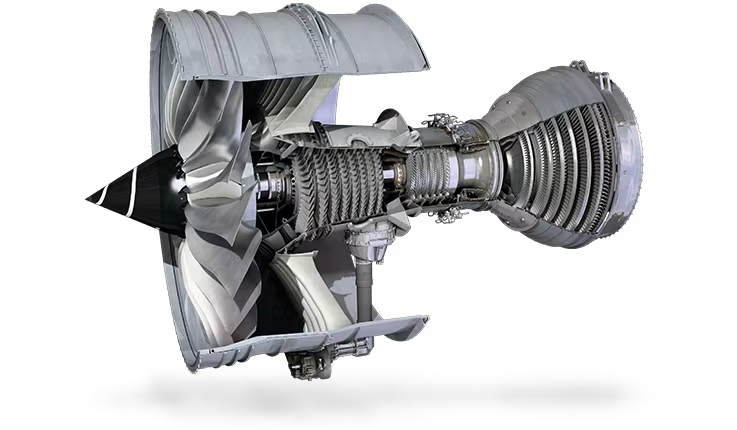
\includegraphics[scale=0.3]{./images/pic/trent-1000.png}
                \end{figure}
            \column{0.1\textwidth}    
            \column{0.5\textwidth}
        \end{columns}
    } 
    \only<2>{
        \begin{columns}
            \column{0.5\textwidth}
                \begin{figure}[H]
                    \centering 
                    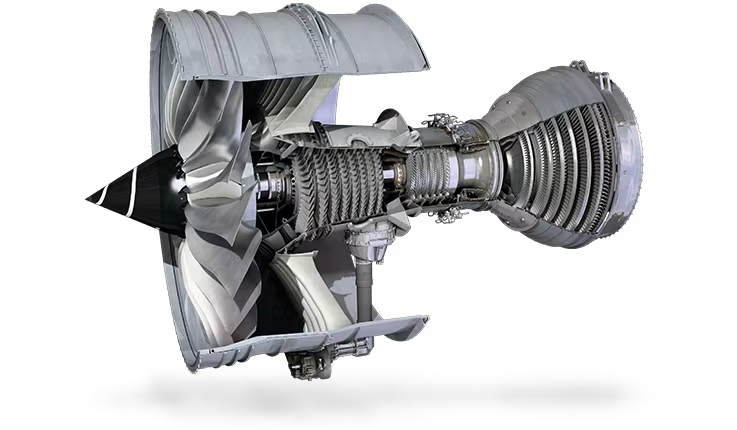
\includegraphics[scale=0.3]{./images/pic/trent-1000.png}
                \end{figure}
            \column{0.1\textwidth}
            \column{0.5\textwidth}
                Current design methods:
                \begin{itemize}
                    \item Iterative processes
                    \item CFD
                    \item Repetitive
                \end{itemize}
        \end{columns}
    } 
    \only<3>{
        \begin{columns}
            \column{0.5\textwidth}
                \begin{figure}[H]
                    \centering 
                    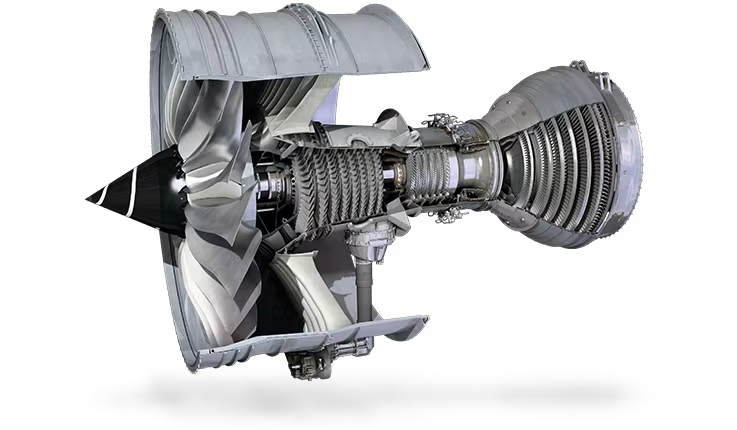
\includegraphics[scale=0.3]{./images/pic/trent-1000.png}
                \end{figure}
            \column{0.1\textwidth}
            \column{0.5\textwidth}
                Current design methods:
                \begin{itemize}
                    \item Iterative processes
                    \item CFD
                    \item Repetitive
                \end{itemize}
                \vspace*{1cm}
                New design method:
                \begin{itemize}
                    \item Physics
                    \item Database
                    \item Machine learning
                \end{itemize}
        \end{columns}
    }
\end{frame}

\begin{frame}{Steps}
    \vspace{-1.5cm}
    \begin{figure}
        \vspace{0.5cm}
        \centering
            \begin{tikzpicture}[
                mindmap,
                every node/.style=concept,
                concept color=black!20,
                grow cyclic,
                level 1/.append style={level distance=8cm, sibling angle=40, font=\small},
                level 2/.append style={level distance=5cm, sibling angle=27, font=\small}
                ]
                \node [root concept, scale=0.85] {{\LARGE\textbf{Data-Driven Design}}} % root
                    child [concept color=yellow, scale=0.5] { node (c1) {\textbf{Machine \\ Learning}}
                        child [rotate=40] { node [scale=0.6] {\textbf{PCA}} }
                        child [rotate=40] { node [scale=0.6] {\textbf{RBF}} }
                    }
                    child [concept color=orange, scale=0.5] { node [level distance=9cm] (c2) {\textbf{Database \\ Generation}} 
                        child [level distance=6cm] { node [scale=0.6, distance=10cm] {\textbf{Strategy}} }
                        child [level distance=6cm] { node [scale=0.6, distance=10cm] {\textbf{Flow Solver}} }
                        child [level distance=6cm] { node [scale=0.6, distance=10cm] {\textbf{Optimizer}} }
                    }
                    child [concept color=red, scale=0.5] { node (c3) {\textbf{Data \\ Setup}}
                    child [rotate=-30] { node [scale = 0.6] {\textbf{Style}} }
                    child [rotate=-30] { node [scale = 0.6] {\textbf{Duty}} }
                    child [rotate=-30] { node [scale = 0.6] {\textbf{Blade}} } 
                    };
                \begin{pgfonlayer}{background}
                    \draw [concept connection]  (c1) edge (c2)
                                                    edge (c3)
                                                (c2) edge (c3);
                    \end{pgfonlayer}
            \end{tikzpicture}
    \end{figure}
\end{frame}

\section{Data Setup}
\SectionPage

\begin{frame}{Steps}
    \vspace{-1.5cm}
    \begin{figure}
        \vspace{0.5cm}
        \centering
            \begin{tikzpicture}[
                mindmap,
                every node/.style=concept,
                concept color=black!20,
                grow cyclic,
                level 1/.append style={level distance=8cm, sibling angle=40, font=\small},
                level 2/.append style={level distance=5cm, sibling angle=27, font=\small}
                ]
                \node [root concept, scale=0.85] {{\LARGE\textbf{Data-Driven Design}}} % root
                    child [concept color=yellow!10, scale=0.5] { node (c1) {\textbf{Machine \\ Learning}}
                        child [rotate=40] { node [scale=0.6] {\textbf{PCA}} }
                        child [rotate=40] { node [scale=0.6] {\textbf{RBF}} }
                    }
                    child [concept color=orange!10, scale=0.5] { node [level distance=9cm] (c2) {\textbf{Database \\ Generation}} 
                        child [level distance=6cm] { node [scale=0.6, distance=10cm] {\textbf{Strategy}} }
                        child [level distance=6cm] { node [scale=0.6, distance=10cm] {\textbf{Flow Solver}} }
                        child [level distance=6cm] { node [scale=0.6, distance=10cm] {\textbf{Optimizer}} }
                    }
                    child [concept color=red, scale=0.5] { node (c3) {\textbf{Data \\ Setup}}
                    child [rotate=-30] { node [scale = 0.6] {\textbf{Style}} }
                    child [rotate=-30] { node [scale = 0.6] {\textbf{Duty}} }
                    child [rotate=-30] { node [scale = 0.6] {\textbf{Blade}} } 
                    };
                \begin{pgfonlayer}{background}
                    \draw [concept connection]  (c1) edge (c2)
                                                     edge (c3)
                                                (c2) edge (c3);
                    \end{pgfonlayer}
            \end{tikzpicture}
    \end{figure}
\end{frame}

\subsection{Data in Turbine Design Process}
\SubSectionPage

\begin{frame}{Turbine design approach}
    \newcommand\WIDTH{7.5cm}
    \newcommand\HEIGHT{2cm}
    \newcommand\Ydist{1cm}
    \newcommand\XPOS{4cm}
    \newcommand\TOTheight{5cm}
    \newcommand\TOTwidth{6cm}
    \newcommand\PTS{2pt}
    \newcommand\SHADOWgray{25}
    \newcommand\PTSin{1pt}
    \newcommand\TRANSPval{0.3}
    \newcommand\BLOCKwidth{1cm}
    \newcommand\BLOCKheight{2cm}
    \newcommand\bigR{3cm}
    \newcommand\medR{2cm}
    \newcommand\lowR{1cm}
    \newcommand\boxW{3cm}
    \newcommand\boxH{2cm}
    \newcommand\leftS{0.5cm}
    \newcommand\physicsDist{0.35cm}
    \newcommand\HspaceVal{-0.3cm}

    \only<1>{
        \begin{figure}
            \centering
            \hspace*{\HspaceVal}
            \begin{tikzpicture}
    
    \node[draw,
        rectangle,
        % rounded corners,
        line width = \PTS,
        minimum height = \TOTheight,
        minimum width = \TOTwidth
    ] (designProcess) at (0, 0) {};

    \node[draw,
        rectangle,
        % rounded corners,
        line width = \PTS,
        minimum height = 1cm,
        minimum width = \TOTwidth,
        above = -\PTS of designProcess.north
    ] (designTitle) {\tiny{\textbf{\tiny{Turbomachine Design Process}}}};

    \node[draw,
        circle, 
        opacity=\TRANSPval,
        line width = \PTS,
        minimum size = \bigR,
        fill = gray!\SHADOWgray,
        right = \physicsDist of designProcess.west
    ] (physics) {\tiny{\textbf{Physics}}};

    \node[draw,
        circle, 
        line width = \PTS,
        opacity=\TRANSPval,
        minimum size = \medR,
        fill = gray!\SHADOWgray,
        above right = 0.5cm and 0.5cm of physics.east
    ] (modeling) {\tiny{\textbf{Modeling}}};

    \node[draw,
        circle, 
        opacity=\TRANSPval,
        line width = \PTS,
        minimum size = \lowR,
        fill = gray!\SHADOWgray,
        below = 1cm of modeling.south
    ] (testing) {\tiny{\textbf{Testing}}};

    \coordinate[left=\leftS of designProcess.west]  (c1) {};
    \coordinate[above=1.5cm of c1]                 (c2) {};
    \coordinate[below=1.5cm of c1]                 (c3) {};
    \coordinate[right=\leftS of designProcess.east] (c4) {};
    \coordinate[above=1.5cm of c4]                 (c5) {};
    \coordinate[below=1.5cm of c4]                 (c6) {};

    \node[draw,
        rectangle,
        opacity=\TRANSPval,
        minimum width = \BLOCKwidth, 
        minimum height = \BLOCKheight, 
        line width = \PTSin,
        left = \leftS of c2
    ] (obj) {\parbox[t][\boxH][c]{\boxW}{
        \tiny{\textbf{Objectives}
        \begin{itemize}
            \item Loss: $Y_p$
            \item Weight
        \end{itemize}  
    }}};

    \node[draw,
        rectangle,
        opacity=\TRANSPval,
        minimum width = \BLOCKwidth, 
        minimum height = \BLOCKheight,
        line width = \PTSin,
        left = \leftS of c3
    ] (constr) {\parbox[t][\boxH][c]{\boxW}{
        \tiny{\textbf{Constraints}
        \begin{itemize}
            \item Turning: $\alpha_1$ \& $\alpha_2$
            \item Flow: $Re$ \& $M_2$
            \item Annlus: $\frac{r_2}{r_1}$
            \item Manufacturing: $\frac{R_{TE}}{c}$
        \end{itemize}  
    }}};

    \node[draw,
        rectangle,
        opacity=\TRANSPval,
        minimum width = \BLOCKwidth, 
        minimum height = \BLOCKheight,
        line width = \PTSin,
        right = \leftS of c5
    ] (obj1) {\parbox[t][\boxH][c]{\boxW}{
        \tiny{\textbf{Objectives}
        \begin{itemize}
            \item Achieved loss: $Y_p$
            \item Achieved weight
        \end{itemize}  
    }}};

    \node[draw,
        rectangle,
        opacity=\TRANSPval,
        minimum width = \BLOCKwidth, 
        minimum height = \BLOCKheight,
        line width = \PTSin,
        right = \leftS of c6
    ] (def) {\parbox[t][\boxH][c]{\boxW}{
        \tiny{\textbf{Definition}
        \begin{itemize}
            \item Blade geometry
        \end{itemize}  
    }}};
    
    \draw[-latex, line width = 2pt, opacity=\TRANSPval] (physics)  to (modeling.west);
    \draw[-latex, line width = 2pt, opacity=\TRANSPval] (modeling) to (testing.north);
    \draw[-latex, line width = 2pt, opacity=\TRANSPval] (testing)  to (physics.south east);
    \draw[-latex, line width = 1pt, opacity=\TRANSPval] (obj.east)    -- (c2) -- (c1) to (designProcess.west);
    \draw[-latex, line width = 1pt, opacity=\TRANSPval] (constr.east) -- (c3) -- (c1) to (designProcess.west);
    \draw[-latex, line width = 1pt, opacity=\TRANSPval] (designProcess.east) -- (c4) -- (c5) to (obj1.west);
    \draw[-latex, line width = 1pt, opacity=\TRANSPval] (designProcess.east) -- (c4) -- (c6) to (def.west);

\end{tikzpicture}
            % 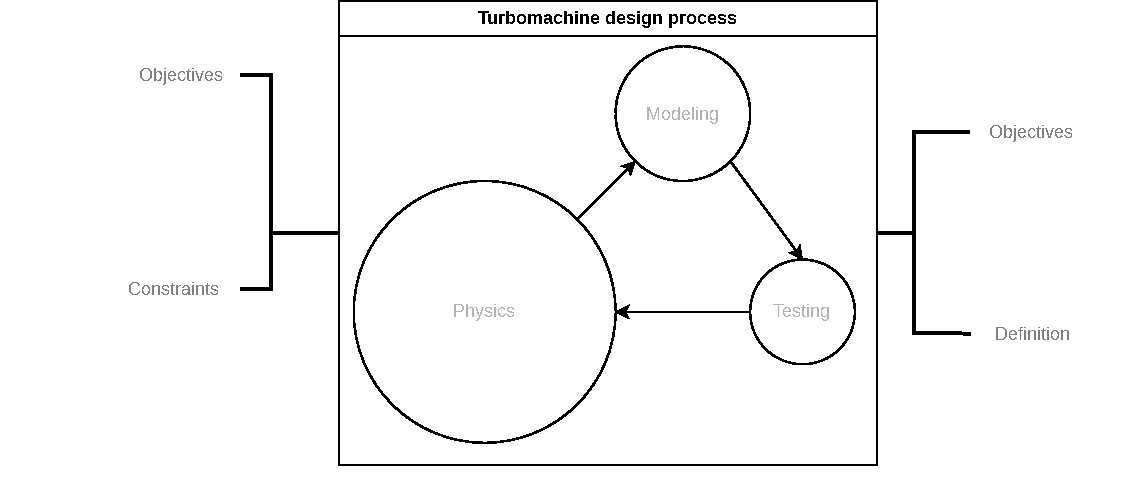
\includegraphics[page=1, scale=0.8]{pdf/turboDesign-00}
        \end{figure}
    }
    \only<2>{
        \begin{figure}
            \centering
            \hspace*{\HspaceVal}
            \begin{tikzpicture}
    
    \node[draw,
        rectangle,
        % rounded corners,
        line width = \PTS,
        minimum height = \TOTheight,
        minimum width = \TOTwidth
    ] (designProcess) at (0, 0) {};

    \node[draw,
        rectangle,
        % rounded corners,
        line width = \PTS,
        minimum height = 1cm,
        minimum width = \TOTwidth,
        above = -\PTS of designProcess.north
    ] (designTitle) {\tiny{\textbf{\tiny{Turbomachine Design Process}}}};

    \node[draw,
        circle, 
        opacity=\TRANSPval,
        line width = \PTS,
        minimum size = \bigR,
        fill = gray!\SHADOWgray,
        right = \physicsDist of designProcess.west
    ] (physics) {\tiny{\textbf{Physics}}};

    \node[draw,
        circle, 
        line width = \PTS,
        opacity=\TRANSPval,
        minimum size = \medR,
        fill = gray!\SHADOWgray,
        above right = 0.5cm and 0.5cm of physics.east
    ] (modeling) {\tiny{\textbf{Modeling}}};

    \node[draw,
        circle, 
        opacity=\TRANSPval,
        line width = \PTS,
        minimum size = \lowR,
        fill = gray!\SHADOWgray,
        below = 1cm of modeling.south
    ] (testing) {\tiny{\textbf{Testing}}};

    \coordinate[left=\leftS of designProcess.west]  (c1) {};
    \coordinate[above=1.5cm of c1]                 (c2) {};
    \coordinate[below=1.5cm of c1]                 (c3) {};
    \coordinate[right=\leftS of designProcess.east] (c4) {};
    \coordinate[above=1.5cm of c4]                 (c5) {};
    \coordinate[below=1.5cm of c4]                 (c6) {};

    \node[draw,
        rectangle,
        % opacity=\TRANSPval,
        minimum width = \BLOCKwidth, 
        minimum height = \BLOCKheight, 
        line width = \PTSin,
        left = \leftS of c2
    ] (obj) {\parbox[t][\boxH][c]{\boxW}{
        \tiny{\textbf{Objectives}
        \begin{itemize}
            \item Loss: $Y_p$
            \item Weight
        \end{itemize}  
    }}};

    \node[draw,
        rectangle,
        opacity=\TRANSPval,
        minimum width = \BLOCKwidth, 
        minimum height = \BLOCKheight,
        line width = \PTSin,
        left = \leftS of c3
    ] (constr) {\parbox[t][\boxH][c]{\boxW}{
        \tiny{\textbf{Constraints}
        \begin{itemize}
            \item Turning: $\alpha_1$ \& $\alpha_2$
            \item Flow: $Re$ \& $M_2$
            \item Annlus: $\frac{r_2}{r_1}$
            \item Manufacturing: $\frac{R_{TE}}{c}$
        \end{itemize}  
    }}};

    \node[draw,
        rectangle,
        opacity=\TRANSPval,
        minimum width = \BLOCKwidth, 
        minimum height = \BLOCKheight,
        line width = \PTSin,
        right = \leftS of c5
    ] (obj1) {\parbox[t][\boxH][c]{\boxW}{
        \tiny{\textbf{Objectives}
        \begin{itemize}
            \item Achieved loss: $Y_p$
            \item Achieved weight
        \end{itemize}  
    }}};

    \node[draw,
        rectangle,
        opacity=\TRANSPval,
        minimum width = \BLOCKwidth, 
        minimum height = \BLOCKheight,
        line width = \PTSin,
        right = \leftS of c6
    ] (def) {\parbox[t][\boxH][c]{\boxW}{
        \tiny{\textbf{Definition}
        \begin{itemize}
            \item Blade geometry
        \end{itemize}  
    }}};
    
    \draw[-latex, line width = 2pt, opacity=\TRANSPval] (physics)  to (modeling.west);
    \draw[-latex, line width = 2pt, opacity=\TRANSPval] (modeling) to (testing.north);
    \draw[-latex, line width = 2pt, opacity=\TRANSPval] (testing)  to (physics.south east);
    \draw[-latex, line width = 1pt] (obj.east)    -- (c2) -- (c1) to (designProcess.west);
    \draw[-latex, line width = 1pt, opacity=\TRANSPval] (constr.east) -- (c3) -- (c1) to (designProcess.west);
    \draw[-latex, line width = 1pt, opacity=\TRANSPval] (designProcess.east) -- (c4) -- (c5) to (obj1.west);
    \draw[-latex, line width = 1pt, opacity=\TRANSPval] (designProcess.east) -- (c4) -- (c6) to (def.west);

\end{tikzpicture}
            % 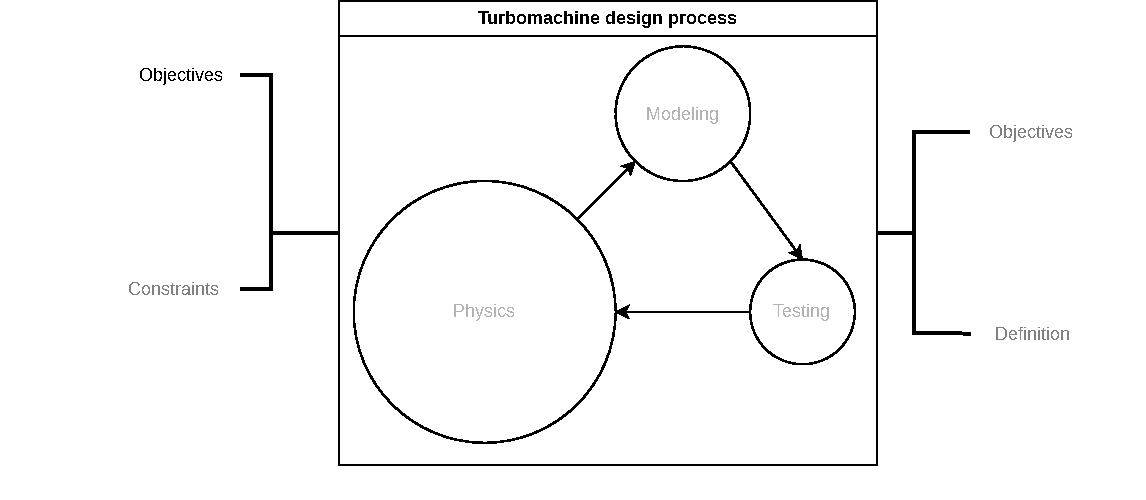
\includegraphics[page=1, scale=0.8]{pdf/turboDesign-01}
        \end{figure}
    }
    \only<3>{
        \begin{figure}
            \centering
            \hspace*{\HspaceVal}
            \begin{tikzpicture}
    
    \node[draw,
        rectangle,
        % rounded corners,
        line width = \PTS,
        minimum height = \TOTheight,
        minimum width = \TOTwidth
    ] (designProcess) at (0, 0) {};

    \node[draw,
        rectangle,
        % rounded corners,
        line width = \PTS,
        minimum height = 1cm,
        minimum width = \TOTwidth,
        above = -\PTS of designProcess.north
    ] (designTitle) {\tiny{\textbf{\tiny{Turbomachine Design Process}}}};

    \node[draw,
        circle, 
        opacity=\TRANSPval,
        line width = \PTS,
        minimum size = \bigR,
        fill = gray!\SHADOWgray,
        right = \physicsDist of designProcess.west
    ] (physics) {\tiny{\textbf{Physics}}};

    \node[draw,
        circle, 
        line width = \PTS,
        opacity=\TRANSPval,
        minimum size = \medR,
        fill = gray!\SHADOWgray,
        above right = 0.5cm and 0.5cm of physics.east
    ] (modeling) {\tiny{\textbf{Modeling}}};

    \node[draw,
        circle, 
        opacity=\TRANSPval,
        line width = \PTS,
        minimum size = \lowR,
        fill = gray!\SHADOWgray,
        below = 1cm of modeling.south
    ] (testing) {\tiny{\textbf{Testing}}};

    \coordinate[left=\leftS of designProcess.west]  (c1) {};
    \coordinate[above=1.5cm of c1]                 (c2) {};
    \coordinate[below=1.5cm of c1]                 (c3) {};
    \coordinate[right=\leftS of designProcess.east] (c4) {};
    \coordinate[above=1.5cm of c4]                 (c5) {};
    \coordinate[below=1.5cm of c4]                 (c6) {};

    \node[draw,
        rectangle,
        % opacity=\TRANSPval,
        minimum width = \BLOCKwidth, 
        minimum height = \BLOCKheight, 
        line width = \PTSin,
        left = \leftS of c2
    ] (obj) {\parbox[t][\boxH][c]{\boxW}{
        \tiny{\textbf{Objectives}
        \begin{itemize}
            \item Loss: $Y_p$
            \item Weight
        \end{itemize}  
    }}};

    \node[draw,
        rectangle,
        % opacity=\TRANSPval,
        minimum width = \BLOCKwidth, 
        minimum height = \BLOCKheight,
        line width = \PTSin,
        left = \leftS of c3
    ] (constr) {\parbox[t][\boxH][c]{\boxW}{
        \tiny{\textbf{Constraints}
        \begin{itemize}
            \item Turning: $\alpha_1$ \& $\alpha_2$
            \item Flow: $Re$ \& $M_2$
            \item Annlus: $\frac{r_2}{r_1}$
            \item Manufacturing: $\frac{R_{TE}}{c}$
        \end{itemize}  
    }}};

    \node[draw,
        rectangle,
        opacity=\TRANSPval,
        minimum width = \BLOCKwidth, 
        minimum height = \BLOCKheight,
        line width = \PTSin,
        right = \leftS of c5
    ] (obj1) {\parbox[t][\boxH][c]{\boxW}{
        \tiny{\textbf{Objectives}
        \begin{itemize}
            \item Achieved loss: $Y_p$
            \item Achieved weight
        \end{itemize}  
    }}};

    \node[draw,
        rectangle,
        opacity=\TRANSPval,
        minimum width = \BLOCKwidth, 
        minimum height = \BLOCKheight,
        line width = \PTSin,
        right = \leftS of c6
    ] (def) {\parbox[t][\boxH][c]{\boxW}{
        \tiny{\textbf{Definition}
        \begin{itemize}
            \item Blade geometry
        \end{itemize}  
    }}};
    
    \draw[-latex, line width = 2pt, opacity=\TRANSPval] (physics)  to (modeling.west);
    \draw[-latex, line width = 2pt, opacity=\TRANSPval] (modeling) to (testing.north);
    \draw[-latex, line width = 2pt, opacity=\TRANSPval] (testing)  to (physics.south east);
    \draw[-latex, line width = 1pt] (obj.east)    -- (c2) -- (c1) to (designProcess.west);
    \draw[-latex, line width = 1pt] (constr.east) -- (c3) -- (c1) to (designProcess.west);
    \draw[-latex, line width = 1pt, opacity=\TRANSPval] (designProcess.east) -- (c4) -- (c5) to (obj1.west);
    \draw[-latex, line width = 1pt, opacity=\TRANSPval] (designProcess.east) -- (c4) -- (c6) to (def.west);

\end{tikzpicture}
            % 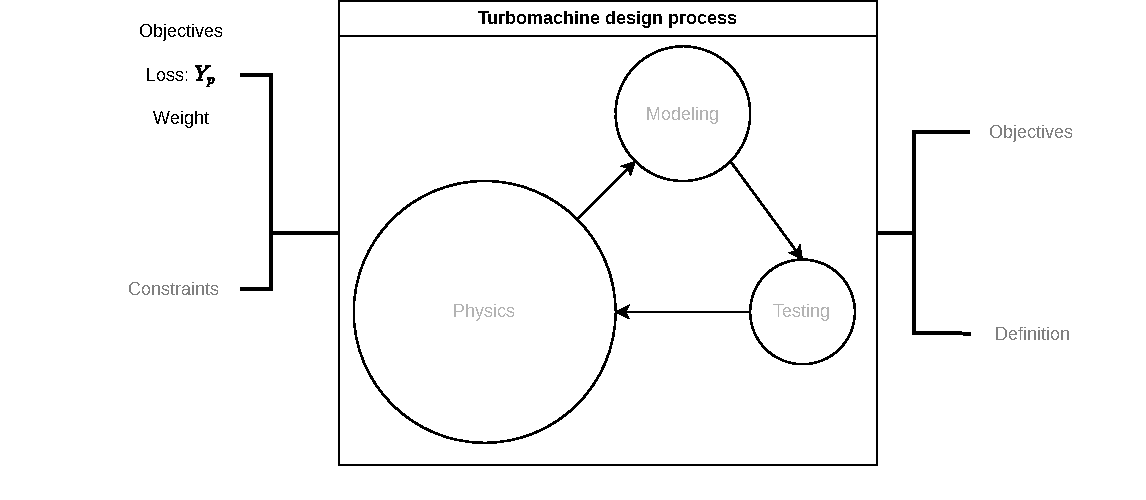
\includegraphics[page=1, scale=0.8]{pdf/turboDesign-02}
        \end{figure}
    }
    \only<4>{
        \begin{figure}
            \centering
            \hspace*{\HspaceVal}
            \begin{tikzpicture}
    
    \node[draw,
        rectangle,
        % rounded corners,
        line width = \PTS,
        minimum height = \TOTheight,
        minimum width = \TOTwidth
    ] (designProcess) at (0, 0) {};

    \node[draw,
        rectangle,
        % rounded corners,
        line width = \PTS,
        minimum height = 1cm,
        minimum width = \TOTwidth,
        above = -\PTS of designProcess.north
    ] (designTitle) {\tiny{\textbf{\tiny{Turbomachine Design Process}}}};

    \node[draw,
        circle, 
        opacity=\TRANSPval,
        line width = \PTS,
        minimum size = \bigR,
        fill = gray!\SHADOWgray,
        right = \physicsDist of designProcess.west
    ] (physics) {\tiny{\textbf{Physics}}};

    \node[draw,
        circle, 
        line width = \PTS,
        opacity=\TRANSPval,
        minimum size = \medR,
        fill = gray!\SHADOWgray,
        above right = 0.5cm and 0.5cm of physics.east
    ] (modeling) {\tiny{\textbf{Modeling}}};

    \node[draw,
        circle, 
        opacity=\TRANSPval,
        line width = \PTS,
        minimum size = \lowR,
        fill = gray!\SHADOWgray,
        below = 1cm of modeling.south
    ] (testing) {\tiny{\textbf{Testing}}};

    \coordinate[left=\leftS of designProcess.west]  (c1) {};
    \coordinate[above=1.5cm of c1]                 (c2) {};
    \coordinate[below=1.5cm of c1]                 (c3) {};
    \coordinate[right=\leftS of designProcess.east] (c4) {};
    \coordinate[above=1.5cm of c4]                 (c5) {};
    \coordinate[below=1.5cm of c4]                 (c6) {};

    \node[draw,
        rectangle,
        % opacity=\TRANSPval,
        minimum width = \BLOCKwidth, 
        minimum height = \BLOCKheight, 
        line width = \PTSin,
        left = \leftS of c2
    ] (obj) {\parbox[t][\boxH][c]{\boxW}{
        \tiny{\textbf{Objectives}
        \begin{itemize}
            \item Loss: $Y_p$
            \item Weight
        \end{itemize}  
    }}};

    \node[draw,
        rectangle,
        % opacity=\TRANSPval,
        minimum width = \BLOCKwidth, 
        minimum height = \BLOCKheight,
        line width = \PTSin,
        left = \leftS of c3
    ] (constr) {\parbox[t][\boxH][c]{\boxW}{
        \tiny{\textbf{Constraints}
        \begin{itemize}
            \item Turning: $\alpha_1$ \& $\alpha_2$
            \item Flow: $Re$ \& $M_2$
            \item Annlus: $\frac{r_2}{r_1}$
            \item Manufacturing: $\frac{R_{TE}}{c}$
        \end{itemize}  
    }}};

    \node[draw,
        rectangle,
        % opacity=\TRANSPval,
        minimum width = \BLOCKwidth, 
        minimum height = \BLOCKheight,
        line width = \PTSin,
        right = \leftS of c5
    ] (obj1) {\parbox[t][\boxH][c]{\boxW}{
        \tiny{\textbf{Objectives}
        \begin{itemize}
            \item Achieved loss: $Y_p$
            \item Achieved weight
        \end{itemize}  
    }}};

    \node[draw,
        rectangle,
        opacity=\TRANSPval,
        minimum width = \BLOCKwidth, 
        minimum height = \BLOCKheight,
        line width = \PTSin,
        right = \leftS of c6
    ] (def) {\parbox[t][\boxH][c]{\boxW}{
        \tiny{\textbf{Definition}
        \begin{itemize}
            \item Blade geometry
        \end{itemize}  
    }}};

    \draw[-latex, line width = 2pt, opacity=\TRANSPval] (physics)  to (modeling.west);
    \draw[-latex, line width = 2pt, opacity=\TRANSPval] (modeling) to (testing.north);
    \draw[-latex, line width = 2pt, opacity=\TRANSPval] (testing)  to (physics.south east);
    \draw[-latex, line width = 1pt] (obj.east)    -- (c2) -- (c1) to (designProcess.west);
    \draw[-latex, line width = 1pt] (constr.east) -- (c3) -- (c1) to (designProcess.west);
    \draw[-latex, line width = 1pt] (designProcess.east) -- (c4) -- (c5) to (obj1.west);
    \draw[-latex, line width = 1pt, opacity=\TRANSPval] (designProcess.east) -- (c4) -- (c6) to (def.west);

\end{tikzpicture}
            % 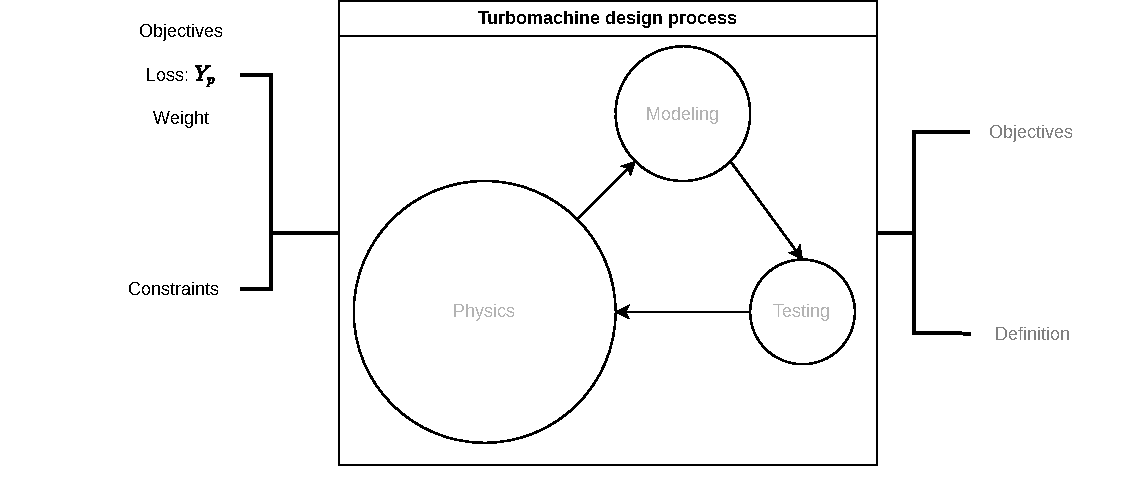
\includegraphics[page=1, scale=0.8]{pdf/turboDesign-03}
        \end{figure}
    }
    \only<5>{
        \begin{figure}
            \centering
            \hspace*{\HspaceVal}
            \begin{tikzpicture}
    
    \node[draw,
        rectangle,
        % rounded corners,
        line width = \PTS,
        minimum height = \TOTheight,
        minimum width = \TOTwidth
    ] (designProcess) at (0, 0) {};

    \node[draw,
        rectangle,
        % rounded corners,
        line width = \PTS,
        minimum height = 1cm,
        minimum width = \TOTwidth,
        above = -\PTS of designProcess.north
    ] (designTitle) {\tiny{\textbf{\tiny{Turbomachine Design Process}}}};

    \node[draw,
        circle, 
        opacity=\TRANSPval,
        line width = \PTS,
        minimum size = \bigR,
        fill = gray!\SHADOWgray,
        right = \physicsDist of designProcess.west
    ] (physics) {\tiny{\textbf{Physics}}};

    \node[draw,
        circle, 
        line width = \PTS,
        opacity=\TRANSPval,
        minimum size = \medR,
        fill = gray!\SHADOWgray,
        above right = 0.5cm and 0.5cm of physics.east
    ] (modeling) {\tiny{\textbf{Modeling}}};

    \node[draw,
        circle, 
        opacity=\TRANSPval,
        line width = \PTS,
        minimum size = \lowR,
        fill = gray!\SHADOWgray,
        below = 1cm of modeling.south
    ] (testing) {\tiny{\textbf{Testing}}};

    \coordinate[left=\leftS of designProcess.west]  (c1) {};
    \coordinate[above=1.5cm of c1]                 (c2) {};
    \coordinate[below=1.5cm of c1]                 (c3) {};
    \coordinate[right=\leftS of designProcess.east] (c4) {};
    \coordinate[above=1.5cm of c4]                 (c5) {};
    \coordinate[below=1.5cm of c4]                 (c6) {};

    \node[draw,
        rectangle,
        % opacity=\TRANSPval,
        minimum width = \BLOCKwidth, 
        minimum height = \BLOCKheight, 
        line width = \PTSin,
        left = \leftS of c2
    ] (obj) {\parbox[t][\boxH][c]{\boxW}{
        \tiny{\textbf{Objectives}
        \begin{itemize}
            \item Loss: $Y_p$
            \item Weight
        \end{itemize}  
    }}};

    \node[draw,
        rectangle,
        % opacity=\TRANSPval,
        minimum width = \BLOCKwidth, 
        minimum height = \BLOCKheight,
        line width = \PTSin,
        left = \leftS of c3
    ] (constr) {\parbox[t][\boxH][c]{\boxW}{
        \tiny{\textbf{Constraints}
        \begin{itemize}
            \item Turning: $\alpha_1$ \& $\alpha_2$
            \item Flow: $Re$ \& $M_2$
            \item Annlus: $\frac{r_2}{r_1}$
            \item Manufacturing: $\frac{R_{TE}}{c}$
        \end{itemize}  
    }}};

    \node[draw,
        rectangle,
        % opacity=\TRANSPval,
        minimum width = \BLOCKwidth, 
        minimum height = \BLOCKheight,
        line width = \PTSin,
        right = \leftS of c5
    ] (obj1) {\parbox[t][\boxH][c]{\boxW}{
        \tiny{\textbf{Objectives}
        \begin{itemize}
            \item Achieved loss: $Y_p$
            \item Achieved weight
        \end{itemize}  
    }}};

    \node[draw,
        rectangle,
        % opacity=\TRANSPval,
        minimum width = \BLOCKwidth, 
        minimum height = \BLOCKheight,
        line width = \PTSin,
        right = \leftS of c6
    ] (def) {\parbox[t][\boxH][c]{\boxW}{
        \tiny{\textbf{Definition}
        \begin{itemize}
            \item Blade geometry
        \end{itemize}  
    }}};
    
    \draw[-latex, line width = 2pt, opacity=\TRANSPval] (physics)  to (modeling.west);
    \draw[-latex, line width = 2pt, opacity=\TRANSPval] (modeling) to (testing.north);
    \draw[-latex, line width = 2pt, opacity=\TRANSPval] (testing)  to (physics.south east);
    \draw[-latex, line width = 1pt] (obj.east)    -- (c2) -- (c1) to (designProcess.west);
    \draw[-latex, line width = 1pt] (constr.east) -- (c3) -- (c1) to (designProcess.west);
    \draw[-latex, line width = 1pt] (designProcess.east) -- (c4) -- (c5) to (obj1.west);
    \draw[-latex, line width = 1pt] (designProcess.east) -- (c4) -- (c6) to (def.west);

\end{tikzpicture}
            % 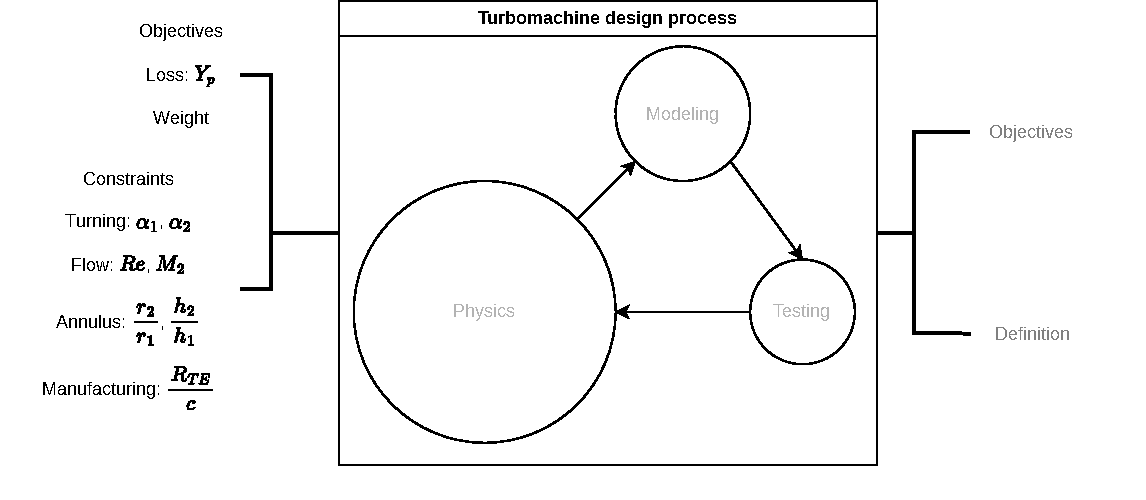
\includegraphics[page=1, scale=0.8]{pdf/turboDesign-04}
        \end{figure}
    }
    \only<6>{
        \begin{figure}
            \centering
            \hspace*{\HspaceVal}
            \begin{tikzpicture}
    
    \node[draw,
        rectangle,
        % rounded corners,
        line width = \PTS,
        minimum height = \TOTheight,
        minimum width = \TOTwidth
    ] (designProcess) at (0, 0) {};

    \node[draw,
        rectangle,
        % rounded corners,
        line width = \PTS,
        minimum height = 1cm,
        minimum width = \TOTwidth,
        above = -\PTS of designProcess.north
    ] (designTitle) {\tiny{\textbf{\tiny{Turbomachine Design Process}}}};

    \node[draw,
        circle, 
        % opacity=\TRANSPval,
        line width = \PTS,
        minimum size = \bigR,
        fill = gray!\SHADOWgray,
        right = \physicsDist of designProcess.west
    ] (physics) {\tiny{\textbf{Physics}}};

    \node[draw,
        circle, 
        line width = \PTS,
        % opacity=\TRANSPval,
        minimum size = \medR,
        fill = gray!\SHADOWgray,
        above right = 0.5cm and 0.5cm of physics.east
    ] (modeling) {\tiny{\textbf{Modeling}}};

    \node[draw,
        circle, 
        % opacity=\TRANSPval,
        line width = \PTS,
        minimum size = \lowR,
        fill = gray!\SHADOWgray,
        below = 1cm of modeling.south
    ] (testing) {\tiny{\textbf{Testing}}};

    \coordinate[left=\leftS of designProcess.west]  (c1) {};
    \coordinate[above=1.5cm of c1]                 (c2) {};
    \coordinate[below=1.5cm of c1]                 (c3) {};
    \coordinate[right=\leftS of designProcess.east] (c4) {};
    \coordinate[above=1.5cm of c4]                 (c5) {};
    \coordinate[below=1.5cm of c4]                 (c6) {};

    \node[draw,
        rectangle,
        % opacity=\TRANSPval,
        minimum width = \BLOCKwidth, 
        minimum height = \BLOCKheight, 
        line width = \PTSin,
        left = \leftS of c2
    ] (obj) {\parbox[t][\boxH][c]{\boxW}{
        \tiny{\textbf{Objectives}
        \begin{itemize}
            \item Loss: $Y_p$
            \item Weight
        \end{itemize}  
    }}};

    \node[draw,
        rectangle,
        % opacity=\TRANSPval,
        minimum width = \BLOCKwidth, 
        minimum height = \BLOCKheight,
        line width = \PTSin,
        left = \leftS of c3
    ] (constr) {\parbox[t][\boxH][c]{\boxW}{
        \tiny{\textbf{Constraints}
        \begin{itemize}
            \item Turning: $\alpha_1$ \& $\alpha_2$
            \item Flow: $Re$ \& $M_2$
            \item Annlus: $\frac{r_2}{r_1}$
            \item Manufacturing: $\frac{R_{TE}}{c}$
        \end{itemize}  
    }}};

    \node[draw,
        rectangle,
        % opacity=\TRANSPval,
        minimum width = \BLOCKwidth, 
        minimum height = \BLOCKheight,
        line width = \PTSin,
        right = \leftS of c5
    ] (obj1) {\parbox[t][\boxH][c]{\boxW}{
        \tiny{\textbf{Objectives}
        \begin{itemize}
            \item Achieved loss: $Y_p$
            \item Achieved weight
        \end{itemize}  
    }}};

    \node[draw,
        rectangle,
        % opacity=\TRANSPval,
        minimum width = \BLOCKwidth, 
        minimum height = \BLOCKheight,
        line width = \PTSin,
        right = \leftS of c6
    ] (def) {\parbox[t][\boxH][c]{\boxW}{
        \tiny{\textbf{Definition}
        \begin{itemize}
            \item Blade geometry
        \end{itemize}  
    }}};
    
    \draw[-latex, line width = 2pt] (physics)  to (modeling.west);
    \draw[-latex, line width = 2pt] (modeling) to (testing.north);
    \draw[-latex, line width = 2pt] (testing)  to (physics.south east);
    \draw[-latex, line width = 1pt] (obj.east)    -- (c2) -- (c1) to (designProcess.west);
    \draw[-latex, line width = 1pt] (constr.east) -- (c3) -- (c1) to (designProcess.west);
    \draw[-latex, line width = 1pt] (designProcess.east) -- (c4) -- (c5) to (obj1.west);
    \draw[-latex, line width = 1pt] (designProcess.east) -- (c4) -- (c6) to (def.west);

\end{tikzpicture}
            % 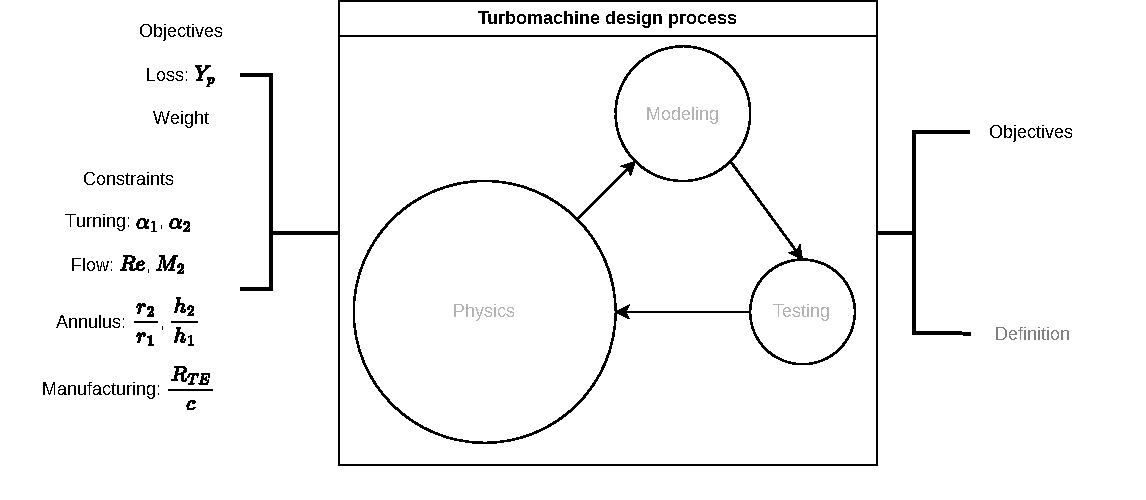
\includegraphics[page=1, scale=0.8]{pdf/turboDesign-05}
        \end{figure}
    }
    % \only<7>{
    %     \begin{figure}
    %         \centering
    %         \hspace*{-1cm}
    %         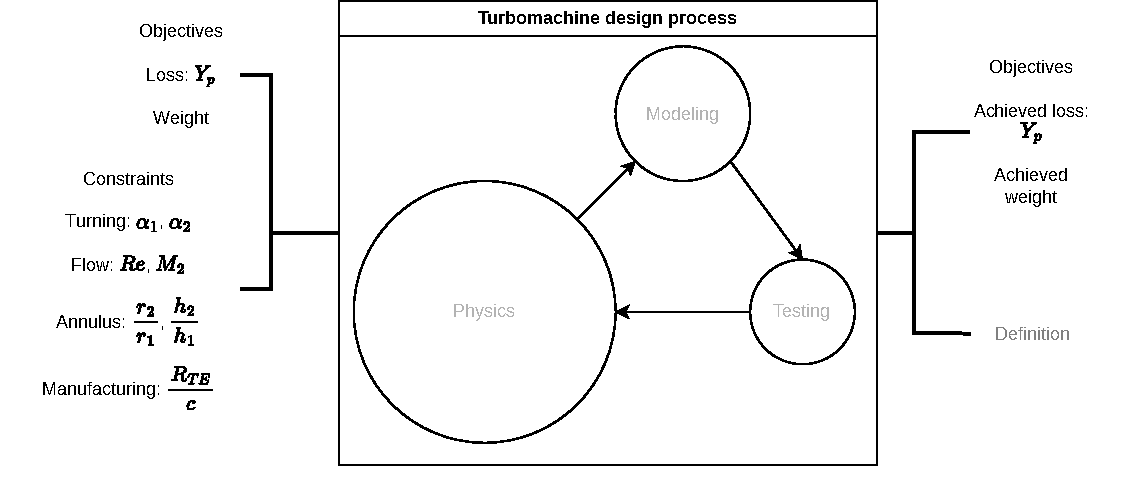
\includegraphics[page=1, scale=0.8]{pdf/turboDesign-06}
    %     \end{figure}
    % }
    % \only<8>{
    %     \begin{figure}
    %         \centering
    %         \hspace*{-1cm}
    %         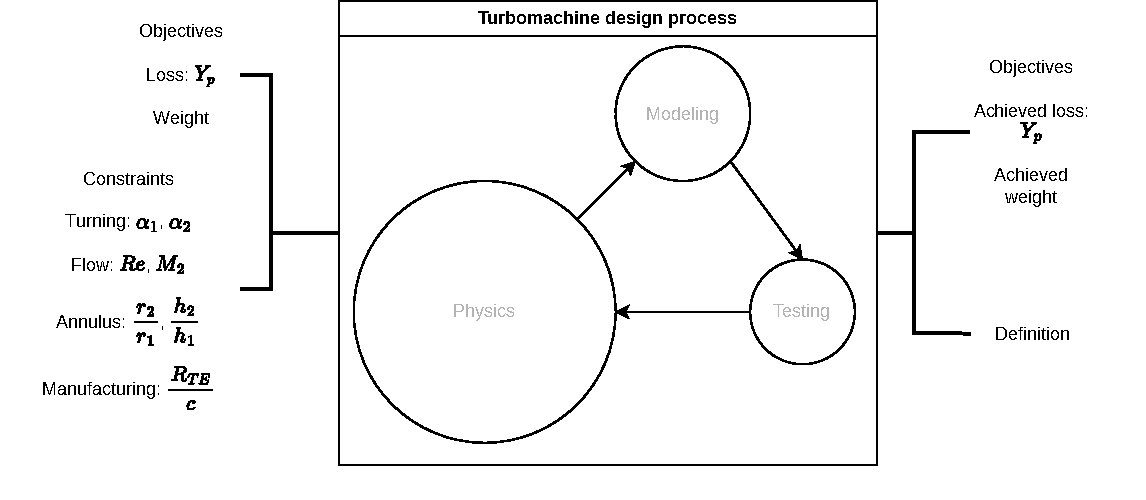
\includegraphics[page=1, scale=0.8]{pdf/turboDesign-07}
    %     \end{figure}
    % }
    % \only<9>{
    %     \begin{figure}
    %         \centering
    %         \hspace*{-1cm}
    %         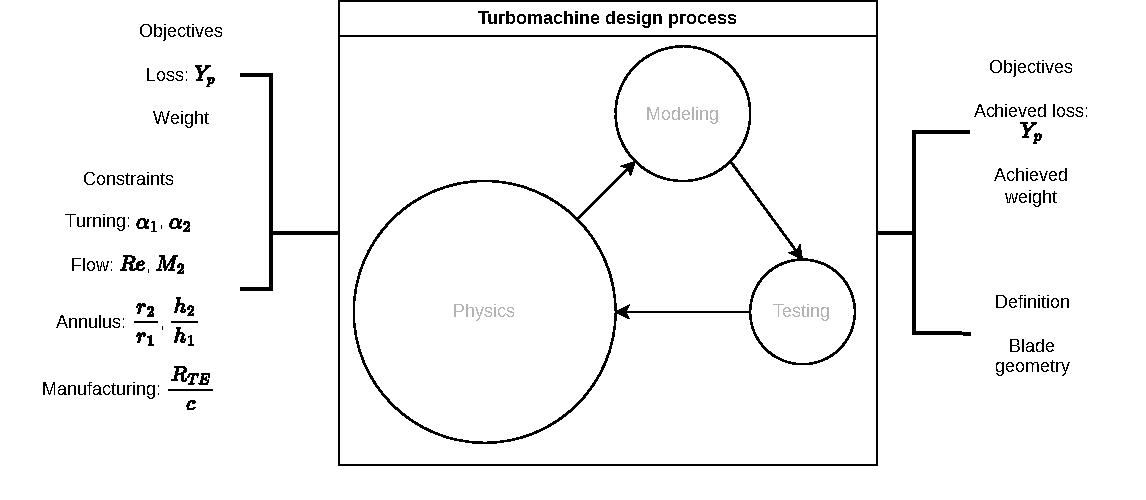
\includegraphics[page=1, scale=0.8]{pdf/turboDesign-08}
    %     \end{figure}
    % }
    % \only<10>{
    %     \begin{figure}
    %         \centering
    %         \hspace*{-1cm}
    %         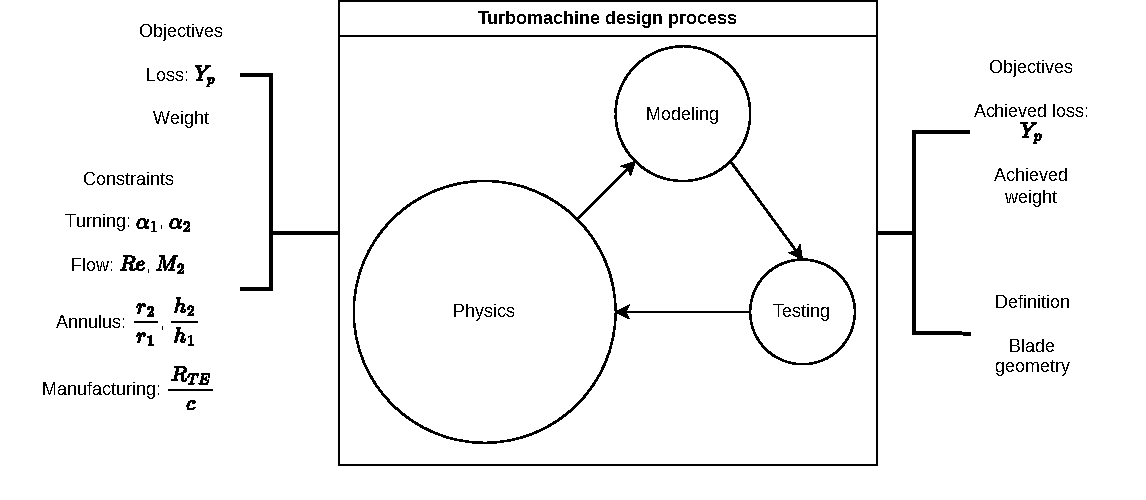
\includegraphics[page=1, scale=0.8]{pdf/turboDesign-09}
    %     \end{figure}
    % }
\end{frame}

\subsection{Tool for Turbine Design}
\SubSectionPage

\begin{frame}{Design process - \Romannum{1}}
    \only<1>{
        \begin{figure}
            \centering
            \newcommand\WIDTH{3cm}
\newcommand\HEIGHT{1.25cm}
\newcommand\Ydist{0.2cm}
\newcommand\XPOS{2cm}
\newcommand\TOTheight{6.2cm}
\newcommand\TOTwidth{3.4cm}
\newcommand\PTS{1.2pt}
\newcommand\SHADOWred{50}
\newcommand\SHADOWgreen{30}
\newcommand\SHADOWblue{20}

\begin{tikzpicture}
    
    \node[draw,
        rectangle,
        % rounded corners,
        line width = \PTS,
        minimum height = \TOTheight,
        minimum width = \TOTwidth
    ] (man) at (0, 0) {};

    \node[draw,
        rectangle,
        % rounded corners,
        line width = \PTS,
        minimum height = \TOTheight,
        minimum width = \TOTwidth,
        right = \XPOS of man
    ] (auto) {};

    % \node[draw,
    %     rectangle,
    %     % rounded corners,
    %     line width = \PTS,
    %     minimum height = \TOTheight,
    %     minimum width = \TOTwidth,
    %     right = \XPOS of auto
    % ] (ml) {};

    \node[draw, 
        rectangle,
        fill = blue!\SHADOWblue,
        line width = \PTS,
        minimum height = 0.8cm,
        above right = -\PTS and 0cm of man.north west
    ] (manTitle) {\textbf{\large{Manual}}};

    \node[draw, 
        rectangle,
        fill = blue!\SHADOWblue,
        line width = \PTS,
        minimum height = 0.8cm,
        above right = -\PTS and 0cm of auto.north west
    ] (autoTitle) {\textbf{\large{Automated}}};

    % \node[draw, 
    %     rectangle,
    %     fill = blue!\SHADOWblue,
    %     line width = \PTS,
    %     minimum height = 1.5cm,
    %     above right = -\PTS and 0cm of ml.north west
    % ] (mlTitle) {\textbf{\Huge{Machine learning}}};

    \node[draw,
        rectangle,
        rounded corners,
        line width = \PTS,
        minimum width = \WIDTH,
        minimum height = \HEIGHT, 
        % fill = red!\SHADOWred,
        below = \Ydist of man.north
    ] (manCFD) {\textbf{\small{Iterative CFD}}};

    \node[draw,
        rectangle,
        rounded corners,
        line width = \PTS,
        minimum width = \WIDTH,
        minimum height = \HEIGHT,
        below = \Ydist of manCFD
    ] (manObj) {\makecell[c]{\textbf{\small{Objectives \&}} \\ \textbf{\small{constraints}}}};%{\textbf{\Large{Objectives \& constraints}}};

    \node[draw,
        rectangle,
        rounded corners,
        line width = \PTS,
        minimum width = \WIDTH,
        minimum height = \HEIGHT,
        below = \Ydist of manObj,
        % fill = green!\SHADOWgreen
    ] (manKnow) {\makecell[c]{\textbf{\small{Using prior}} \\ \textbf{\small{knowledge}}}}; %{\textbf{Using prior knowledge}};

    \node[draw,
        rectangle,
        rounded corners,
        line width = \PTS,
        minimum width = \WIDTH,
        minimum height = \HEIGHT,
        below = \Ydist of manKnow,
        % fill = red!\SHADOWred
    ] (manMan) {\textbf{\small{Manual}}};

    \node[draw,
        rectangle,
        rounded corners,
        line width = \PTS,
        minimum width = \WIDTH,
        minimum height = \HEIGHT, 
        below = \Ydist of auto.north,
        % fill = red!\SHADOWred
    ] (autoCFD) {\textbf{\small{Iterative CFD}}};

    \node[draw,
        rectangle,
        rounded corners,
        line width = \PTS,
        minimum width = \WIDTH,
        minimum height = \HEIGHT,
        below = \Ydist of autoCFD
    ] (autoObj) {\makecell[c]{\textbf{\small{Objectives \&}} \\ \textbf{\small{constraints}}}};%{\textbf{\Large{Objectives \& constraints}}};

    \node[draw,
        rectangle,
        rounded corners,
        line width = \PTS,
        minimum width = \WIDTH,
        minimum height = \HEIGHT,
        below = \Ydist of autoObj,
        % fill = red!\SHADOWred
    ] (autoKnow) {\makecell[c]{\textbf{\small{Not using prior}} \\ \textbf{\small{knowledge}}}};

    \node[draw,
        rectangle,
        rounded corners,
        line width = \PTS,
        minimum width = \WIDTH,
        minimum height = \HEIGHT,
        below = \Ydist of autoKnow,
        % fill = green!\SHADOWgreen
    ] (autoAuto) {\textbf{\small{Automated}}}; 

    % \node[draw,
    %     rectangle,
    %     rounded corners,
    %     line width = \PTS,
    %     minimum width = \WIDTH
    %     minimum height = \HEIGHT, 
    %     below = \Ydist of ml.north,
    %     fill = green!\SHADOWgreen
    % ] (mlCFD) {\textbf{\Large{Regression}}};

    % \node[draw,
    %     rectangle,
    %     rounded corners,
    %     line width = \PTS,
    %     minimum width = \WIDTH,
    %     minimum height = \HEIGHT,
    %     below = \Ydist of mlCFD,
    %     fill = green!\SHADOWgreen
    % ] (mlObj) {\makecell[c]{\textbf{\Large{Aerodynamic duty \&}} \\ \textbf{\Large{aerodynamic style}}}};%{\textbf{\Large{Objectives \& constraints}}};

    % \node[draw,
    %     rectangle,
    %     rounded corners,
    %     line width = \PTS,
    %     minimum width = \WIDTH,
    %     minimum height = \HEIGHT,
    %     below = \Ydist of mlObj,
    %     fill = green!\SHADOWgreen
    % ] (mlKnow) {\makecell[c]{\textbf{\Large{Using prior}} \\ \textbf{\Large{knowledge}}}};

    % \node[draw,
    %     rectangle,
    %     rounded corners,
    %     line width = \PTS,
    %     minimum width = \WIDTH,
    %     minimum height = \HEIGHT,
    %     below = \Ydist of mlKnow,
    %     fill = green!\SHADOWgreen
    % ] (mlAuto) {\textbf{\Large{Automated}}}; 
 
\end{tikzpicture}

            % 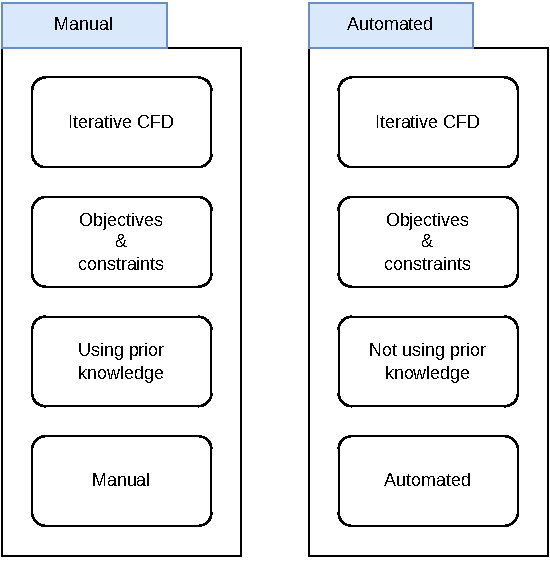
\includegraphics[page=1, scale=0.75]{pdf/designModes-00}
        \end{figure}
    }
    \only<2>{
        \begin{figure}
            \centering
            \newcommand\WIDTH{3cm}
\newcommand\HEIGHT{1.25cm}
\newcommand\Ydist{0.2cm}
\newcommand\XPOS{2cm}
\newcommand\TOTheight{6.2cm}
\newcommand\TOTwidth{3.4cm}
\newcommand\PTS{1.2pt}
\newcommand\SHADOWred{50}
\newcommand\SHADOWgreen{30}
\newcommand\SHADOWblue{20}

\begin{tikzpicture}
    
    \node[draw,
        rectangle,
        % rounded corners,
        line width = \PTS,
        minimum height = \TOTheight,
        minimum width = \TOTwidth
    ] (man) at (0, 0) {};

    \node[draw,
        rectangle,
        % rounded corners,
        line width = \PTS,
        minimum height = \TOTheight,
        minimum width = \TOTwidth,
        right = \XPOS of man
    ] (auto) {};

    % \node[draw,
    %     rectangle,
    %     % rounded corners,
    %     line width = \PTS,
    %     minimum height = \TOTheight,
    %     minimum width = \TOTwidth,
    %     right = \XPOS of auto
    % ] (ml) {};

    \node[draw, 
        rectangle,
        fill = blue!\SHADOWblue,
        line width = \PTS,
        minimum height = 0.8cm,
        above right = -\PTS and 0cm of man.north west
    ] (manTitle) {\textbf{\large{Manual}}};

    \node[draw, 
        rectangle,
        fill = blue!\SHADOWblue,
        line width = \PTS,
        minimum height = 0.8cm,
        above right = -\PTS and 0cm of auto.north west
    ] (autoTitle) {\textbf{\large{Automated}}};

    % \node[draw, 
    %     rectangle,
    %     fill = blue!\SHADOWblue,
    %     line width = \PTS,
    %     minimum height = 1.5cm,
    %     above right = -\PTS and 0cm of ml.north west
    % ] (mlTitle) {\textbf{\Huge{Machine learning}}};

    \node[draw,
        rectangle,
        rounded corners,
        line width = \PTS,
        minimum width = \WIDTH,
        minimum height = \HEIGHT, 
        fill = red!\SHADOWred,
        below = \Ydist of man.north
    ] (manCFD) {\textbf{\small{Iterative CFD}}};

    \node[draw,
        rectangle,
        rounded corners,
        line width = \PTS,
        minimum width = \WIDTH,
        minimum height = \HEIGHT,
        below = \Ydist of manCFD
    ] (manObj) {\makecell[c]{\textbf{\small{Objectives \&}} \\ \textbf{\small{constraints}}}};%{\textbf{\Large{Objectives \& constraints}}};

    \node[draw,
        rectangle,
        rounded corners,
        line width = \PTS,
        minimum width = \WIDTH,
        minimum height = \HEIGHT,
        below = \Ydist of manObj,
        fill = green!\SHADOWgreen
    ] (manKnow) {\makecell[c]{\textbf{\small{Using prior}} \\ \textbf{\small{knowledge}}}}; %{\textbf{Using prior knowledge}};

    \node[draw,
        rectangle,
        rounded corners,
        line width = \PTS,
        minimum width = \WIDTH,
        minimum height = \HEIGHT,
        below = \Ydist of manKnow,
        fill = red!\SHADOWred
    ] (manMan) {\textbf{\small{Manual}}};

    \node[draw,
        rectangle,
        rounded corners,
        line width = \PTS,
        minimum width = \WIDTH,
        minimum height = \HEIGHT, 
        below = \Ydist of auto.north,
        fill = red!\SHADOWred
    ] (autoCFD) {\textbf{\small{Iterative CFD}}};

    \node[draw,
        rectangle,
        rounded corners,
        line width = \PTS,
        minimum width = \WIDTH,
        minimum height = \HEIGHT,
        below = \Ydist of autoCFD
    ] (autoObj) {\makecell[c]{\textbf{\small{Objectives \&}} \\ \textbf{\small{constraints}}}};%{\textbf{\Large{Objectives \& constraints}}};

    \node[draw,
        rectangle,
        rounded corners,
        line width = \PTS,
        minimum width = \WIDTH,
        minimum height = \HEIGHT,
        below = \Ydist of autoObj,
        fill = red!\SHADOWred
    ] (autoKnow) {\makecell[c]{\textbf{\small{Not using prior}} \\ \textbf{\small{knowledge}}}};

    \node[draw,
        rectangle,
        rounded corners,
        line width = \PTS,
        minimum width = \WIDTH,
        minimum height = \HEIGHT,
        below = \Ydist of autoKnow,
        fill = green!\SHADOWgreen
    ] (autoAuto) {\textbf{\small{Automated}}}; 

    % \node[draw,
    %     rectangle,
    %     rounded corners,
    %     line width = \PTS,
    %     minimum width = \WIDTH
    %     minimum height = \HEIGHT, 
    %     below = \Ydist of ml.north,
    %     fill = green!\SHADOWgreen
    % ] (mlCFD) {\textbf{\Large{Regression}}};

    % \node[draw,
    %     rectangle,
    %     rounded corners,
    %     line width = \PTS,
    %     minimum width = \WIDTH,
    %     minimum height = \HEIGHT,
    %     below = \Ydist of mlCFD,
    %     fill = green!\SHADOWgreen
    % ] (mlObj) {\makecell[c]{\textbf{\Large{Aerodynamic duty \&}} \\ \textbf{\Large{aerodynamic style}}}};%{\textbf{\Large{Objectives \& constraints}}};

    % \node[draw,
    %     rectangle,
    %     rounded corners,
    %     line width = \PTS,
    %     minimum width = \WIDTH,
    %     minimum height = \HEIGHT,
    %     below = \Ydist of mlObj,
    %     fill = green!\SHADOWgreen
    % ] (mlKnow) {\makecell[c]{\textbf{\Large{Using prior}} \\ \textbf{\Large{knowledge}}}};

    % \node[draw,
    %     rectangle,
    %     rounded corners,
    %     line width = \PTS,
    %     minimum width = \WIDTH,
    %     minimum height = \HEIGHT,
    %     below = \Ydist of mlKnow,
    %     fill = green!\SHADOWgreen
    % ] (mlAuto) {\textbf{\Large{Automated}}}; 
 
\end{tikzpicture}

            % 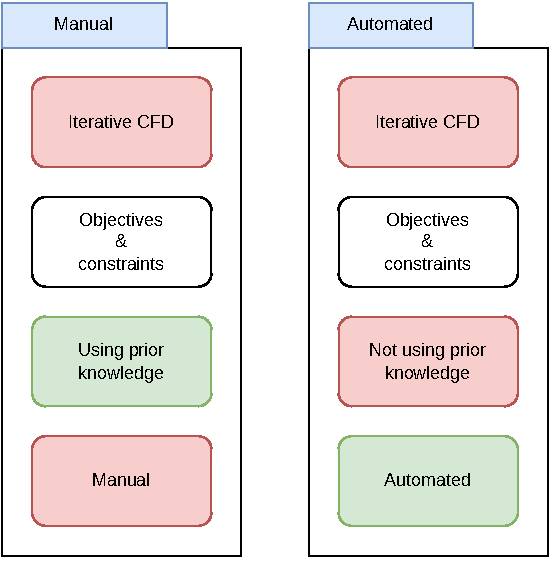
\includegraphics[page=1, scale=0.75]{pdf/designModes-01}
        \end{figure}
    }
    \only<3>{
        \begin{figure}
            \centering
            \newcommand\WIDTH{3cm}
\newcommand\HEIGHT{1.25cm}
\newcommand\Ydist{0.2cm}
\newcommand\XPOS{2cm}
\newcommand\TOTheight{6.2cm}
\newcommand\TOTwidth{3.4cm}
\newcommand\PTS{1.2pt}
\newcommand\SHADOWred{50}
\newcommand\SHADOWgreen{30}
\newcommand\SHADOWblue{20}

\vspace{-0.5cm}

\begin{tikzpicture}
    
    \node[draw,
        rectangle,
        % rounded corners,
        line width = \PTS,
        minimum height = \TOTheight,
        minimum width = \TOTwidth
    ] (man) at (0, 0) {};

    \node[draw,
        rectangle,
        % rounded corners,
        line width = \PTS,
        minimum height = \TOTheight,
        minimum width = \TOTwidth,
        right = \XPOS of man
    ] (auto) {};

    \node[draw,
        rectangle,
        % rounded corners,
        line width = \PTS,
        minimum height = \TOTheight,
        minimum width = \TOTwidth,
        right = \XPOS of auto
    ] (ml) {};

    \node[draw, 
        rectangle,
        fill = blue!\SHADOWblue,
        line width = \PTS,
        minimum height = 0.8cm,
        above right = -\PTS and 0cm of man.north west
    ] (manTitle) {\textbf{\small{Manual}}};

    \node[draw, 
        rectangle,
        fill = blue!\SHADOWblue,
        line width = \PTS,
        minimum height = 0.8cm,
        above right = -\PTS and 0cm of auto.north west
    ] (autoTitle) {\textbf{\small{Automated}}};

    \node[draw, 
        rectangle,
        fill = blue!\SHADOWblue,
        line width = \PTS,
        minimum height = 0.8cm,
        above right = -\PTS and 0cm of ml.north west
    ] (mlTitle) {\textbf{\small{Machine learning}}};

    \node[draw,
        rectangle,
        rounded corners,
        line width = \PTS,
        minimum width = \WIDTH,
        minimum height = \HEIGHT, 
        % fill = red!\SHADOWred,
        below = \Ydist of man.north
    ] (manCFD) {\textbf{\small{Iterative CFD}}};

    \node[draw,
        rectangle,
        rounded corners,
        line width = \PTS,
        minimum width = \WIDTH,
        minimum height = \HEIGHT,
        below = \Ydist of manCFD
    ] (manObj) {\makecell[c]{\textbf{\small{Objectives \&}} \\ \textbf{\small{constraints}}}};%{\textbf{\small{Objectives \& constraints}}};

    \node[draw,
        rectangle,
        rounded corners,
        line width = \PTS,
        minimum width = \WIDTH,
        minimum height = \HEIGHT,
        below = \Ydist of manObj,
        fill = green!\SHADOWgreen
    ] (manKnow) {\makecell[c]{\textbf{\small{Using prior}} \\ \textbf{\small{knowledge}}}}; %{\textbf{Using prior knowledge}};

    \node[draw,
        rectangle,
        rounded corners,
        line width = \PTS,
        minimum width = \WIDTH,
        minimum height = \HEIGHT,
        below = \Ydist of manKnow,
        % fill = red!\SHADOWred
    ] (manMan) {\textbf{\small{Manual}}};

    \node[draw,
        rectangle,
        rounded corners,
        line width = \PTS,
        minimum width = \WIDTH,
        minimum height = \HEIGHT, 
        below = \Ydist of auto.north,
        % fill = red!\SHADOWred
    ] (autoCFD) {\textbf{\small{Iterative CFD}}};

    \node[draw,
        rectangle,
        rounded corners,
        line width = \PTS,
        minimum width = \WIDTH,
        minimum height = \HEIGHT,
        below = \Ydist of autoCFD
    ] (autoObj) {\makecell[c]{\textbf{\small{Objectives \&}} \\ \textbf{\small{constraints}}}};%{\textbf{\small{Objectives \& constraints}}};

    \node[draw,
        rectangle,
        rounded corners,
        line width = \PTS,
        minimum width = \WIDTH,
        minimum height = \HEIGHT,
        below = \Ydist of autoObj,
        % fill = red!\SHADOWred
    ] (autoKnow) {\makecell[c]{\textbf{\small{Not using prior}} \\ \textbf{\small{knowledge}}}};

    \node[draw,
        rectangle,
        rounded corners,
        line width = \PTS,
        minimum width = \WIDTH,
        minimum height = \HEIGHT,
        below = \Ydist of autoKnow,
        fill = green!\SHADOWgreen
    ] (autoAuto) {\textbf{\small{Automated}}}; 

    \node[draw,
        rectangle,
        rounded corners,
        line width = \PTS,
        minimum width = \WIDTH,
        minimum height = \HEIGHT, 
        below = \Ydist of ml.north,
        % fill = green!\SHADOWgreen
    ] (mlCFD) {};%{\textbf{\small{Regression}}};

    \node[draw,
        rectangle,
        rounded corners,
        line width = \PTS,
        minimum width = \WIDTH,
        minimum height = \HEIGHT,
        below = \Ydist of mlCFD,
        % fill = green!\SHADOWgreen
    ] (mlObj) {};%{\makecell[c]{\textbf{\small{Aerodynamic duty \&}} \\ \textbf{\small{aerodynamic style}}}};%{\textbf{\small{Objectives \& constraints}}};

    \node[draw,
        rectangle,
        rounded corners,
        line width = \PTS,
        minimum width = \WIDTH,
        minimum height = \HEIGHT,
        below = \Ydist of mlObj,
        fill = green!\SHADOWgreen
    ] (mlKnow) {\makecell[c]{\textbf{\small{Using prior}} \\ \textbf{\small{knowledge}}}};

    \node[draw,
        rectangle,
        rounded corners,
        line width = \PTS,
        minimum width = \WIDTH,
        minimum height = \HEIGHT,
        below = \Ydist of mlKnow,
        fill = green!\SHADOWgreen
    ] (mlAuto) {\textbf{\small{Automated}}}; 
 
\end{tikzpicture}

            % 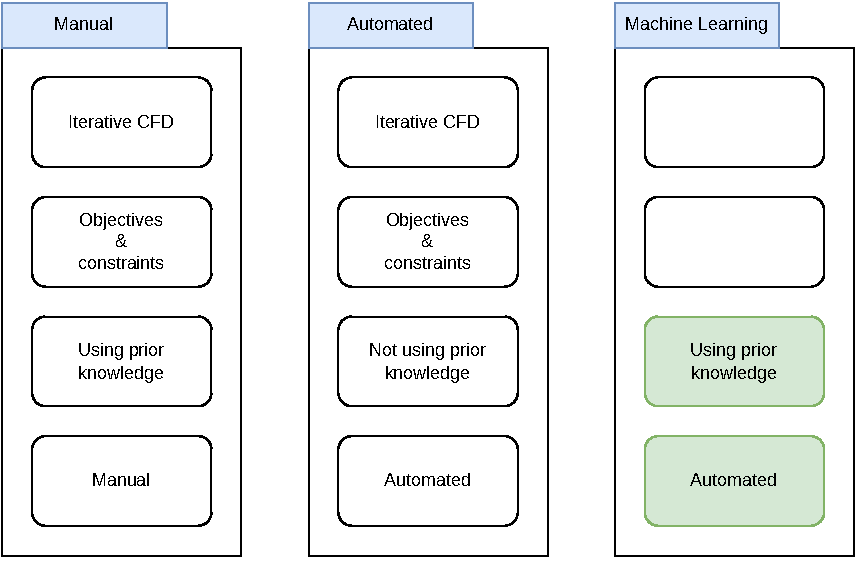
\includegraphics[page=1, scale=0.75]{pdf/designModes-02}
        \end{figure}
    }
\end{frame}

\begin{frame}{Data in turbomachinery design}
    \vspace{0.5cm}
    These points allow to use a \textbf{regression based model} to design a blade.
    \vspace{0.5cm}
    \begin{itemize}
        \setlength{\itemsep}{15pt}
        \item Turbomachinery design physics \textbf{is not stochastic}
        \item Turbomachinery design is \textbf{multi-objectives} and \textbf{multi-constrained}
        \item Turbomachinery blades are \textbf{high dimensional objects}
    \end{itemize}
    \vspace{0.5cm}
    The blade has to be parametrized by \textbf{few parameters} after a \textbf{design space reduction}. \\
    
    \vspace{0.5cm}
    Data collection has to \textbf{correlate} the \textbf{design objectives} to the \textbf{blade geometry}.
\end{frame}

\begin{frame}{Design process - \Romannum{2}}
    \begin{figure}
        \centering
        \newcommand\WIDTH{3cm}
\newcommand\HEIGHT{1.25cm}
\newcommand\Ydist{0.2cm}
\newcommand\XPOS{2cm}
\newcommand\TOTheight{6.2cm}
\newcommand\TOTwidth{3.4cm}
\newcommand\PTS{1.2pt}
\newcommand\SHADOWred{50}
\newcommand\SHADOWgreen{30}
\newcommand\SHADOWblue{20}

\vspace{-0.5cm}

\begin{tikzpicture}
    
    \node[draw,
        rectangle,
        % rounded corners,
        line width = \PTS,
        minimum height = \TOTheight,
        minimum width = \TOTwidth
    ] (man) at (0, 0) {};

    \node[draw,
        rectangle,
        % rounded corners,
        line width = \PTS,
        minimum height = \TOTheight,
        minimum width = \TOTwidth,
        right = \XPOS of man
    ] (auto) {};

    \node[draw,
        rectangle,
        % rounded corners,
        line width = \PTS,
        minimum height = \TOTheight,
        minimum width = \TOTwidth,
        right = \XPOS of auto
    ] (ml) {};

    \node[draw, 
        rectangle,
        fill = blue!\SHADOWblue,
        line width = \PTS,
        minimum height = 0.8cm,
        above right = -\PTS and 0cm of man.north west
    ] (manTitle) {\textbf{\small{Manual}}};

    \node[draw, 
        rectangle,
        fill = blue!\SHADOWblue,
        line width = \PTS,
        minimum height = 0.8cm,
        above right = -\PTS and 0cm of auto.north west
    ] (autoTitle) {\textbf{\small{Automated}}};

    \node[draw, 
        rectangle,
        fill = blue!\SHADOWblue,
        line width = \PTS,
        minimum height = 0.8cm,
        above right = -\PTS and 0cm of ml.north west
    ] (mlTitle) {\textbf{\small{Machine learning}}};

    \node[draw,
        rectangle,
        rounded corners,
        line width = \PTS,
        minimum width = \WIDTH,
        minimum height = \HEIGHT, 
        % fill = red!\SHADOWred,
        below = \Ydist of man.north
    ] (manCFD) {\textbf{\small{Iterative CFD}}};

    \node[draw,
        rectangle,
        rounded corners,
        line width = \PTS,
        minimum width = \WIDTH,
        minimum height = \HEIGHT,
        below = \Ydist of manCFD
    ] (manObj) {\makecell[c]{\textbf{\small{Objectives \&}} \\ \textbf{\small{constraints}}}};%{\textbf{\small{Objectives \& constraints}}};

    \node[draw,
        rectangle,
        rounded corners,
        line width = \PTS,
        minimum width = \WIDTH,
        minimum height = \HEIGHT,
        below = \Ydist of manObj,
        fill = green!\SHADOWgreen
    ] (manKnow) {\makecell[c]{\textbf{\small{Using prior}} \\ \textbf{\small{knowledge}}}}; %{\textbf{Using prior knowledge}};

    \node[draw,
        rectangle,
        rounded corners,
        line width = \PTS,
        minimum width = \WIDTH,
        minimum height = \HEIGHT,
        below = \Ydist of manKnow,
        % fill = red!\SHADOWred
    ] (manMan) {\textbf{\small{Manual}}};

    \node[draw,
        rectangle,
        rounded corners,
        line width = \PTS,
        minimum width = \WIDTH,
        minimum height = \HEIGHT, 
        below = \Ydist of auto.north,
        % fill = red!\SHADOWred
    ] (autoCFD) {\textbf{\small{Iterative CFD}}};

    \node[draw,
        rectangle,
        rounded corners,
        line width = \PTS,
        minimum width = \WIDTH,
        minimum height = \HEIGHT,
        below = \Ydist of autoCFD
    ] (autoObj) {\makecell[c]{\textbf{\small{Objectives \&}} \\ \textbf{\small{constraints}}}};%{\textbf{\small{Objectives \& constraints}}};

    \node[draw,
        rectangle,
        rounded corners,
        line width = \PTS,
        minimum width = \WIDTH,
        minimum height = \HEIGHT,
        below = \Ydist of autoObj,
        % fill = red!\SHADOWred
    ] (autoKnow) {\makecell[c]{\textbf{\small{Not using prior}} \\ \textbf{\small{knowledge}}}};

    \node[draw,
        rectangle,
        rounded corners,
        line width = \PTS,
        minimum width = \WIDTH,
        minimum height = \HEIGHT,
        below = \Ydist of autoKnow,
        fill = green!\SHADOWgreen
    ] (autoAuto) {\textbf{\small{Automated}}}; 

    \node[draw,
        rectangle,
        rounded corners,
        line width = \PTS,
        minimum width = \WIDTH,
        minimum height = \HEIGHT, 
        below = \Ydist of ml.north,
        fill = green!\SHADOWgreen
    ] (mlCFD) {\textbf{\small{Regression}}};

    \node[draw,
        rectangle,
        rounded corners,
        line width = \PTS,
        minimum width = \WIDTH,
        minimum height = \HEIGHT,
        below = \Ydist of mlCFD,
        % fill = green!\SHADOWgreen
    ] (mlObj) {};%{\makecell[c]{\textbf{\small{Aerodynamic duty \&}} \\ \textbf{\small{aerodynamic style}}}};%{\textbf{\small{Objectives \& constraints}}};

    \node[draw,
        rectangle,
        rounded corners,
        line width = \PTS,
        minimum width = \WIDTH,
        minimum height = \HEIGHT,
        below = \Ydist of mlObj,
        fill = green!\SHADOWgreen
    ] (mlKnow) {\makecell[c]{\textbf{\small{Using prior}} \\ \textbf{\small{knowledge}}}};

    \node[draw,
        rectangle,
        rounded corners,
        line width = \PTS,
        minimum width = \WIDTH,
        minimum height = \HEIGHT,
        below = \Ydist of mlKnow,
        fill = green!\SHADOWgreen
    ] (mlAuto) {\textbf{\small{Automated}}}; 
 
\end{tikzpicture}

        % 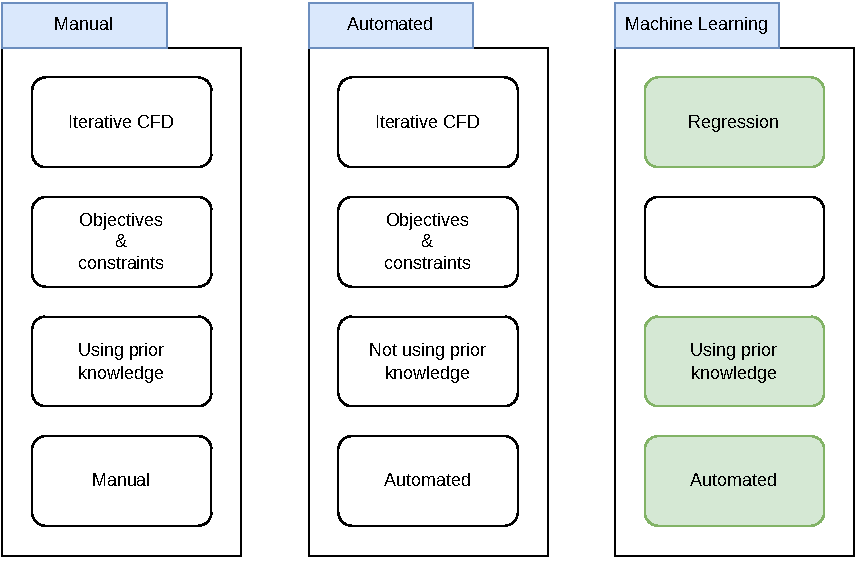
\includegraphics[page=1, scale=0.75]{pdf/designModes-03}
    \end{figure}
\end{frame}

\begin{frame}{Data features}
    \vspace{0.5cm}
    % The design tool \textbf{does not have objectives neither constraints}. 
    % \newline
    % \vspace{0.2cm}
    
    The computed data has to \textbf{map} the objective domain satisfying the constraints. 
    \newline
    \vspace{0.2cm}
    
    This can be achieved using appropriate \textbf{design features}.
    \newline
    \vspace{0.2cm}
    
    In order to collect all these information, the data will depend on two new \textbf{aerodynamic features}: 
    \newline
    \vspace{0.2cm}

    \begin{itemize}
        \setlength{\itemsep}{15pt}
        \item \textbf{Aerodynamic duty}: a domain of study that allows \textbf{mapping} the constraints
        \item \textbf{Aerodynamic style}: a domain of study that allows \textbf{mapping} the objectives
    \end{itemize} 
\end{frame}

\begin{frame}{Design process - \Romannum{3}}
    \begin{figure}
        \centering
        \newcommand\WIDTH{3cm}
\newcommand\HEIGHT{1.25cm}
\newcommand\Ydist{0.2cm}
\newcommand\XPOS{2cm}
\newcommand\TOTheight{6.2cm}
\newcommand\TOTwidth{3.4cm}
\newcommand\PTS{1.2pt}
\newcommand\SHADOWred{50}
\newcommand\SHADOWgreen{30}
\newcommand\SHADOWblue{20}

\vspace{-0.5cm}

\begin{tikzpicture}
    
    \node[draw,
        rectangle,
        % rounded corners,
        line width = \PTS,
        minimum height = \TOTheight,
        minimum width = \TOTwidth
    ] (man) at (0, 0) {};

    \node[draw,
        rectangle,
        % rounded corners,
        line width = \PTS,
        minimum height = \TOTheight,
        minimum width = \TOTwidth,
        right = \XPOS of man
    ] (auto) {};

    \node[draw,
        rectangle,
        % rounded corners,
        line width = \PTS,
        minimum height = \TOTheight,
        minimum width = \TOTwidth,
        right = \XPOS of auto
    ] (ml) {};

    \node[draw, 
        rectangle,
        fill = blue!\SHADOWblue,
        line width = \PTS,
        minimum height = 0.8cm,
        above right = -\PTS and 0cm of man.north west
    ] (manTitle) {\textbf{\small{Manual}}};

    \node[draw, 
        rectangle,
        fill = blue!\SHADOWblue,
        line width = \PTS,
        minimum height = 0.8cm,
        above right = -\PTS and 0cm of auto.north west
    ] (autoTitle) {\textbf{\small{Automated}}};

    \node[draw, 
        rectangle,
        fill = blue!\SHADOWblue,
        line width = \PTS,
        minimum height = 0.8cm,
        above right = -\PTS and 0cm of ml.north west
    ] (mlTitle) {\textbf{\small{Machine learning}}};

    \node[draw,
        rectangle,
        rounded corners,
        line width = \PTS,
        minimum width = \WIDTH,
        minimum height = \HEIGHT, 
        % fill = red!\SHADOWred,
        below = \Ydist of man.north
    ] (manCFD) {\textbf{\small{Iterative CFD}}};

    \node[draw,
        rectangle,
        rounded corners,
        line width = \PTS,
        minimum width = \WIDTH,
        minimum height = \HEIGHT,
        below = \Ydist of manCFD
    ] (manObj) {\makecell[c]{\textbf{\small{Objectives \&}} \\ \textbf{\small{constraints}}}};%{\textbf{\small{Objectives \& constraints}}};

    \node[draw,
        rectangle,
        rounded corners,
        line width = \PTS,
        minimum width = \WIDTH,
        minimum height = \HEIGHT,
        below = \Ydist of manObj,
        fill = green!\SHADOWgreen
    ] (manKnow) {\makecell[c]{\textbf{\small{Using prior}} \\ \textbf{\small{knowledge}}}}; %{\textbf{Using prior knowledge}};

    \node[draw,
        rectangle,
        rounded corners,
        line width = \PTS,
        minimum width = \WIDTH,
        minimum height = \HEIGHT,
        below = \Ydist of manKnow,
        % fill = red!\SHADOWred
    ] (manMan) {\textbf{\small{Manual}}};

    \node[draw,
        rectangle,
        rounded corners,
        line width = \PTS,
        minimum width = \WIDTH,
        minimum height = \HEIGHT, 
        below = \Ydist of auto.north,
        % fill = red!\SHADOWred
    ] (autoCFD) {\textbf{\small{Iterative CFD}}};

    \node[draw,
        rectangle,
        rounded corners,
        line width = \PTS,
        minimum width = \WIDTH,
        minimum height = \HEIGHT,
        below = \Ydist of autoCFD
    ] (autoObj) {\makecell[c]{\textbf{\small{Objectives \&}} \\ \textbf{\small{constraints}}}};%{\textbf{\small{Objectives \& constraints}}};

    \node[draw,
        rectangle,
        rounded corners,
        line width = \PTS,
        minimum width = \WIDTH,
        minimum height = \HEIGHT,
        below = \Ydist of autoObj,
        % fill = red!\SHADOWred
    ] (autoKnow) {\makecell[c]{\textbf{\small{Not using prior}} \\ \textbf{\small{knowledge}}}};

    \node[draw,
        rectangle,
        rounded corners,
        line width = \PTS,
        minimum width = \WIDTH,
        minimum height = \HEIGHT,
        below = \Ydist of autoKnow,
        fill = green!\SHADOWgreen
    ] (autoAuto) {\textbf{\small{Automated}}}; 

    \node[draw,
        rectangle,
        rounded corners,
        line width = \PTS,
        minimum width = \WIDTH,
        minimum height = \HEIGHT, 
        below = \Ydist of ml.north,
        fill = green!\SHADOWgreen
    ] (mlCFD) {\textbf{\small{Regression}}};

    \node[draw,
        rectangle,
        rounded corners,
        line width = \PTS,
        minimum width = \WIDTH,
        minimum height = \HEIGHT,
        below = \Ydist of mlCFD,
        fill = green!\SHADOWgreen
    ] (mlObj) {\makecell[c]{\textbf{\small{Aerodynamic}} \\ \textbf{\small{duty \& style}}}};%{\textbf{\small{Objectives \& constraints}}};

    \node[draw,
        rectangle,
        rounded corners,
        line width = \PTS,
        minimum width = \WIDTH,
        minimum height = \HEIGHT,
        below = \Ydist of mlObj,
        fill = green!\SHADOWgreen
    ] (mlKnow) {\makecell[c]{\textbf{\small{Using prior}} \\ \textbf{\small{knowledge}}}};

    \node[draw,
        rectangle,
        rounded corners,
        line width = \PTS,
        minimum width = \WIDTH,
        minimum height = \HEIGHT,
        below = \Ydist of mlKnow,
        fill = green!\SHADOWgreen
    ] (mlAuto) {\textbf{\small{Automated}}}; 
 
\end{tikzpicture}

        % 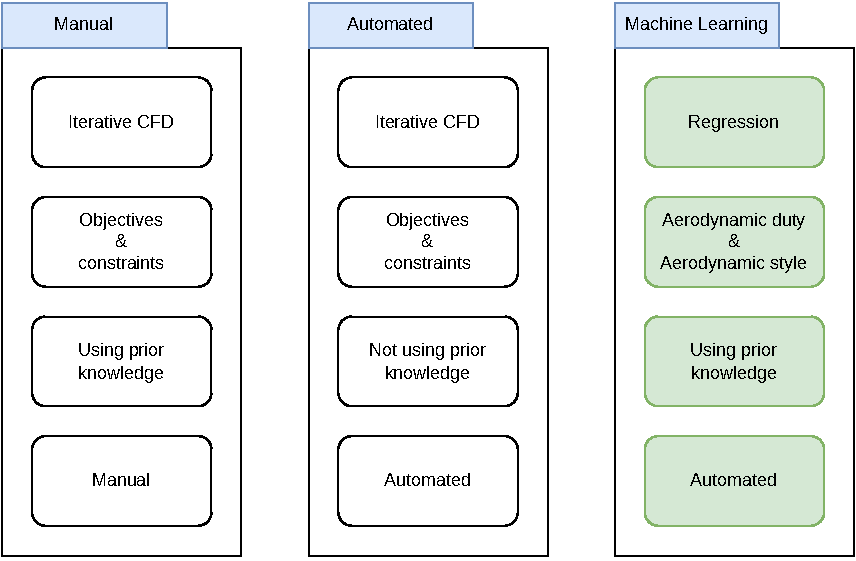
\includegraphics[page=1, scale=0.75]{pdf/designModes-04}
    \end{figure}
\end{frame}

\subsection{Blade Parametrization}
\SubSectionPage

\subsubsection{Camberline Parametrization}

%% Disable the logo in the lower right corner:
% \hidelogo

\hidelogo
% \begin{frame}{Camberline parametrization}
%     \vspace{-0.5cm}
%     \begin{columns}
%         \column{0.5\textwidth}
%             \begin{block}{Camberline parameters}
%                 \begin{itemize}
%                     \item $\chi_1$: metal inlet angle
%                     \item $\chi_2$: metal outlet angle 
%                     \item $\gamma$: stagger angle
%                 \end{itemize}
%             \end{block}
%             \vspace{-0.4cm}
%             \begin{block}{Camberline formulation}
%                 \tiny{
%                 \begin{itemize}
%                     % \item $a = a_{(\chi_1, \chi_2, \gamma)}$
%                     % \item $b = b_{(\chi_1, \chi_2, \gamma)}$
%                     % \item $n = n_{(\chi_1, \chi_2, \gamma)}$
%                     \item $n = \frac{tan(\chi_2) + tan(\chi_1)}{tan(\gamma)}$
%                     \item $a = \frac{tan(\chi_2)}{n}$
%                     \item $b =  - \frac{tan(\chi_1)}{n}$
%                     \item $y = a \cdot x^n + b \cdot (1 - x)^n$
%                     \item $y^{\prime} = a \cdot n \cdot x^{n-1} - b \cdot n \cdot (1 - x)^{n - 1}$
%                     \item $\boldsymbol{n} = 
%                     \begin{bmatrix}
%                         - \frac{y^{\prime}}{\sqrt{1 + (y^{\prime})^2}} \\
%                         \frac{1}{\sqrt{1 + (y^{\prime})^2}}
%                     \end{bmatrix}$
%                 \end{itemize}
%                 }
%             \end{block}
%         \column{0.5\textwidth}
%             % \begin{block}{Camberline variables}
%                 % \begin{itemize}
%                     % \item $n = \frac{tan(\chi_2) + tan(\chi_1)}{tan(\gamma)}$
%                     % \item $a = \frac{tan(\chi_2)}{n}$
%                     % \item $b =  - \frac{tan(\chi_1)}{n}$
%                 % \end{itemize}
%             % \end{block}
%             \begin{figure}
%                 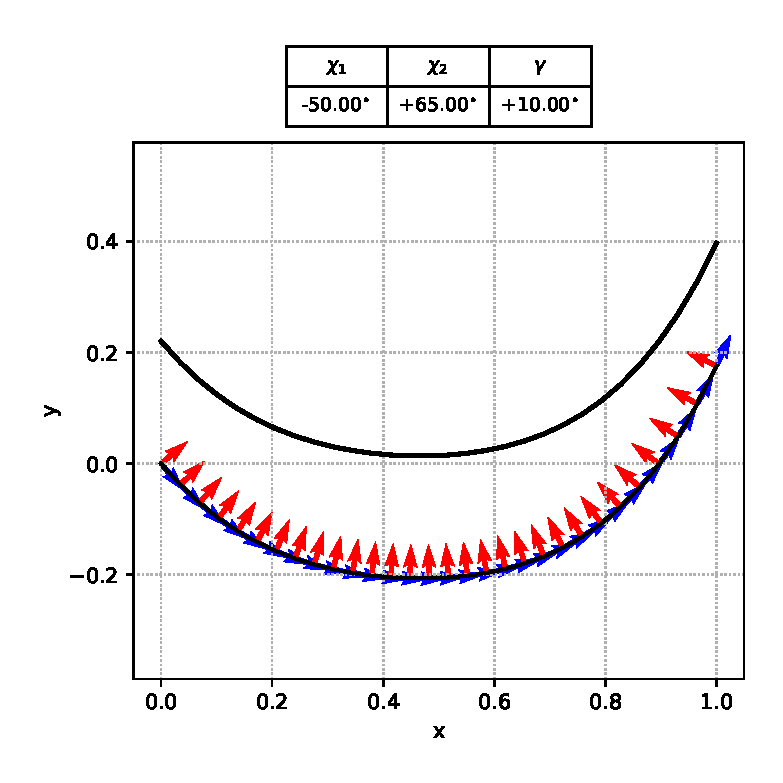
\includegraphics[width=0.8\textwidth]{images/camberline/camberline01.eps}
%             \end{figure}
%     \end{columns}
% \end{frame}   

\begin{frame}{Camberline parametrization}
    \vspace{-0.5cm}
    \begin{columns}
        \column{0.5\textwidth}
            \begin{figure}
                \centering
                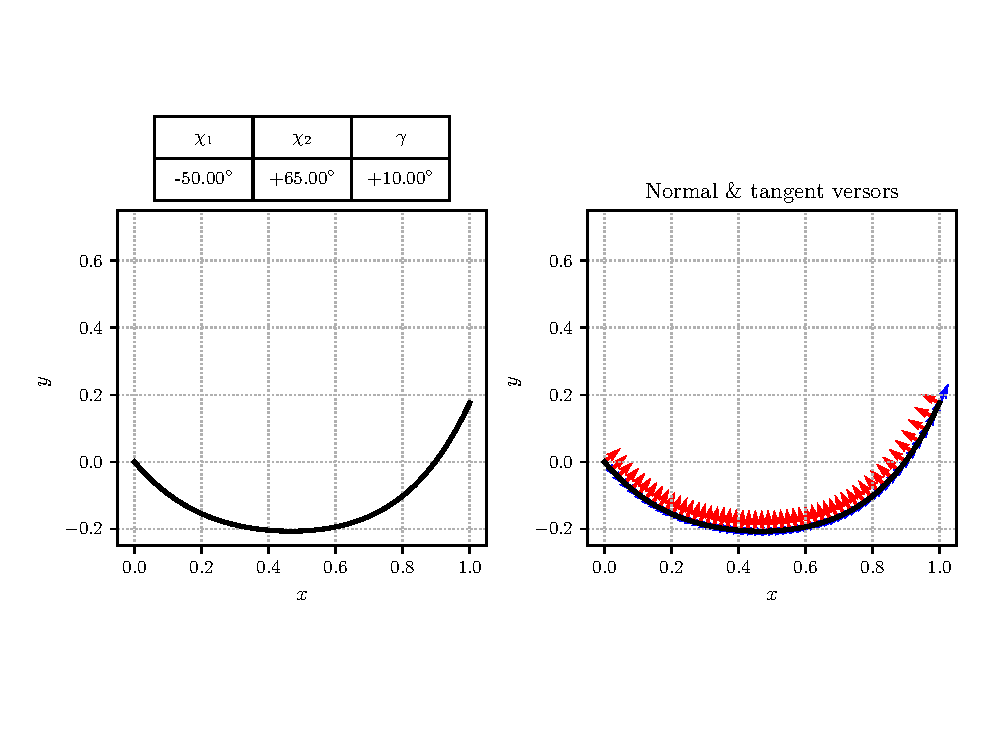
\includegraphics[width=\textwidth]{./images/cLine1.eps}
            \end{figure}
        \column{0.5\textwidth}
            \begin{figure}
                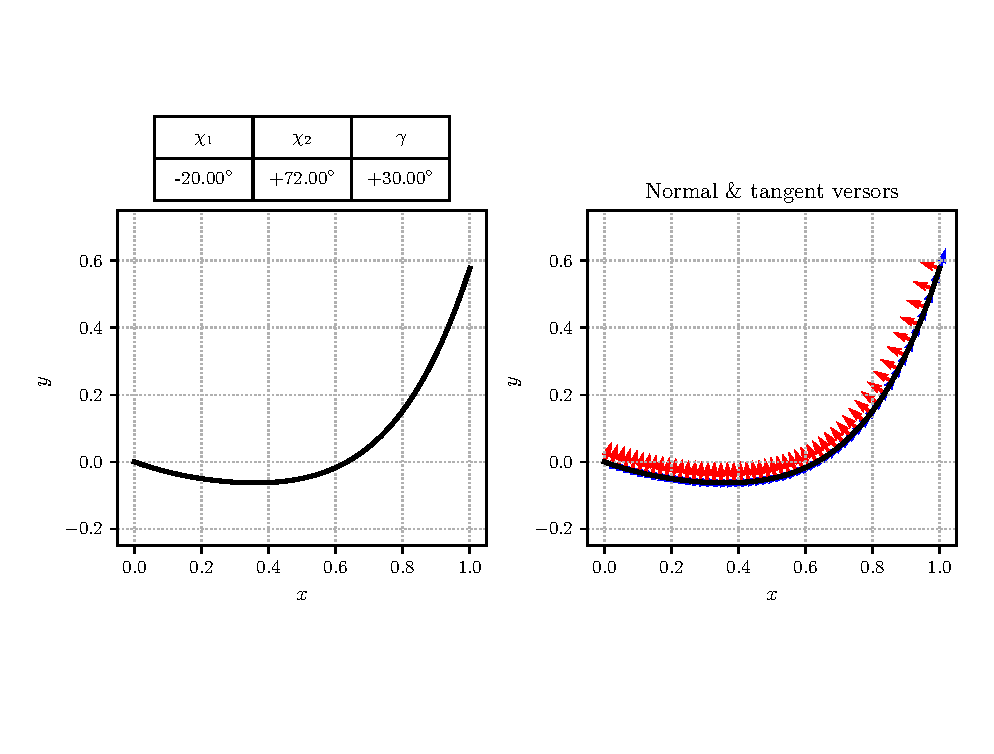
\includegraphics[width=\textwidth]{./images/cLine2.eps}
            \end{figure}
    \end{columns}
\end{frame}   

% \subsubsection{Profile Parametrization}
% \begin{frame}{Profile parametrization}
%     \vspace{1cm}
%     \begin{block}{Profile thickness, $\zeta$}
%         Kulfan parametrization studies the thickness distribution using shape functions.
%         \begin{itemize}
%             \setlength\itemsep{0.3cm}
%             \item Class function: $C_{(x)}$
%             \item Shape function: $S_{(x, i, N)}$
%             \item Trailing edge radius thickness distribution: $\zeta_{TE} \cdot x$
%             \item Total shape function: $\zeta_{(x)}$
%         \end{itemize}
%     \end{block}

%     % \begin{block}{Profile properties}
%         % \begin{itemize}
%             % \item Thickness distribution with respect to the Bernstein function: $S_{(x, 0, 2)}$                 
%             % \item The trailing edge radius thickness, $\zeta_{TE_{(x)}}$, is been added normally to the camberline using a linear distribution 
%             % \item The leading edge radius is expressed only by the $A_0$ parameter
%             % \item The wedge angle, $\beta$, is expressed only by the $A_N$ parameter
%         % \end{itemize}
%     % \end{block}
% \end{frame}

\begin{frame}{Bernstein functions and class function}
    % \vspace{-4cm}
    \begin{columns}
        \column{0.5\textwidth}
        \vspace{-0.5cm} 
        \begin{equation*}
            S_{(x, i, N)} = A_i \cdot \frac{N!}{(N - i)! \cdot i!} \cdot x^i \cdot (1 - x)^{N - 1}
        \end{equation*}
        \vspace{-0.5cm}
        \begin{figure}
            % 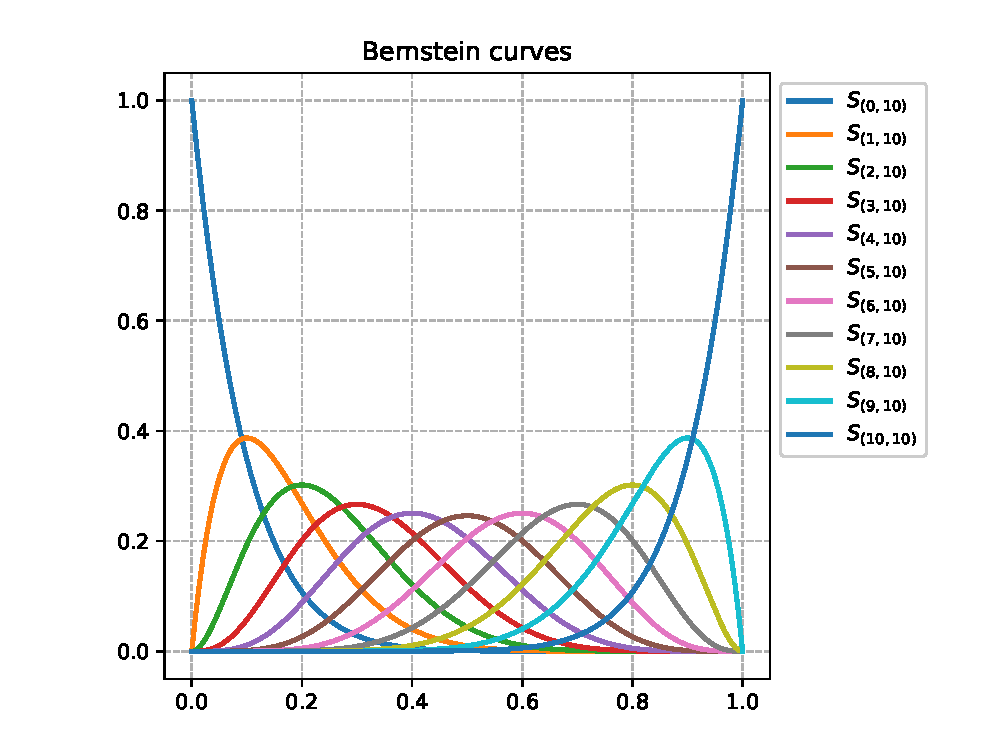
\includegraphics[width=\textwidth]{images/profileLine/bernstein.eps}
            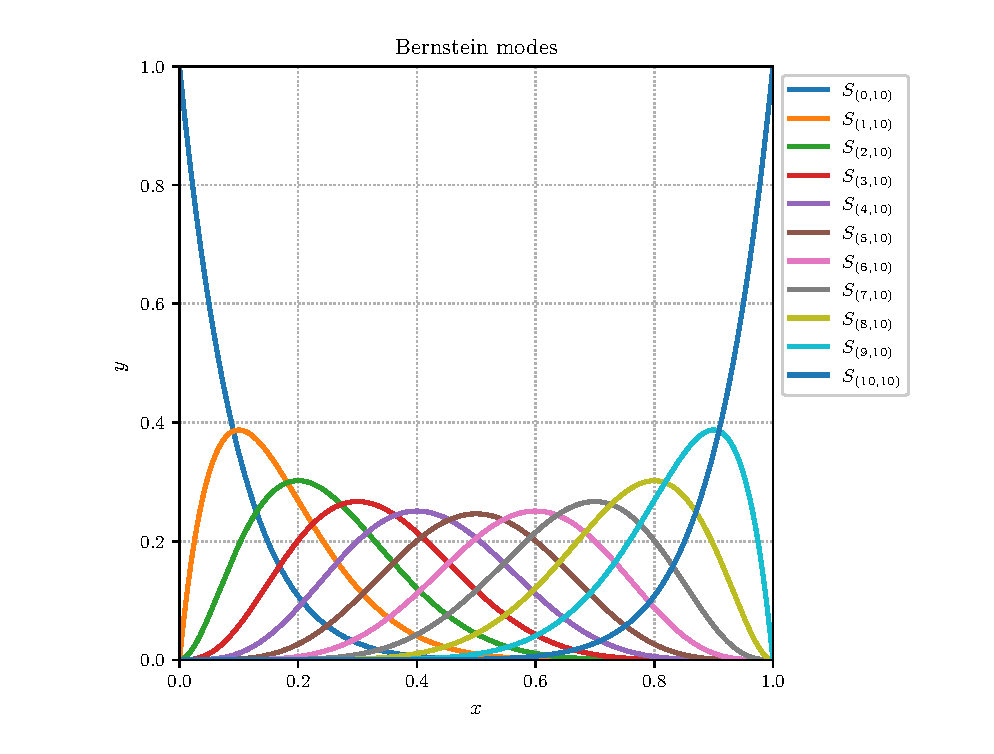
\includegraphics[width=\textwidth]{./images/bernstein.eps}
        \end{figure}
        \column{0.5\textwidth}
        \begin{equation*}
            C_{(x)} = x^{0.5} \cdot (1 - x)^{1.0}
        \end{equation*}
        \begin{figure}
            % 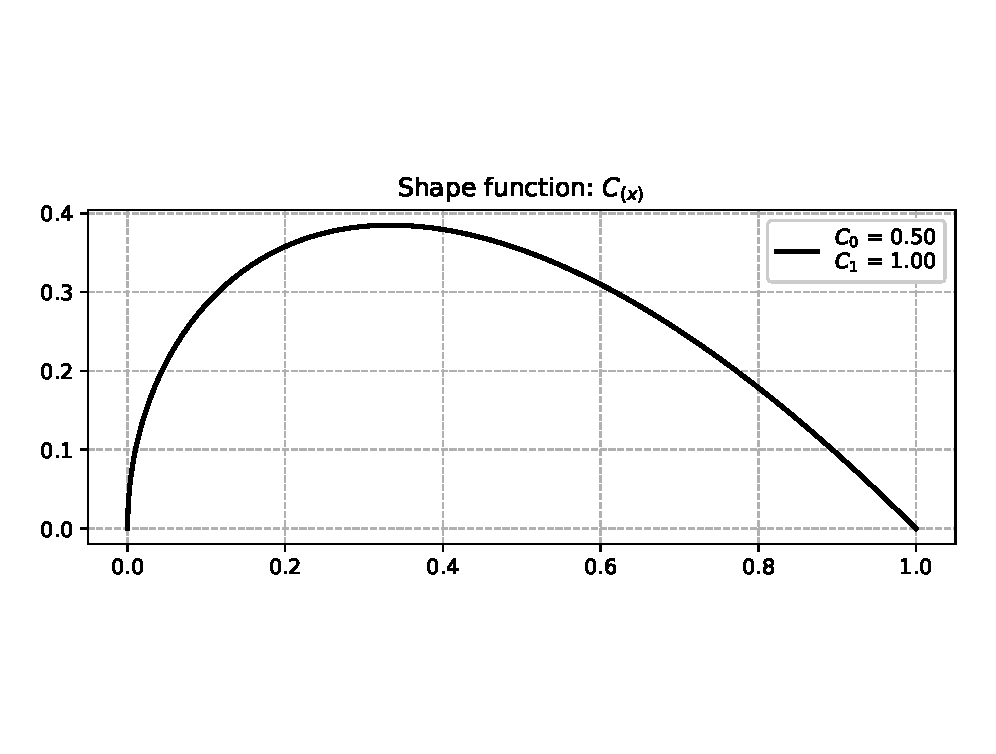
\includegraphics[width=\textwidth]{images/profileLine/shapeFunction.eps}
            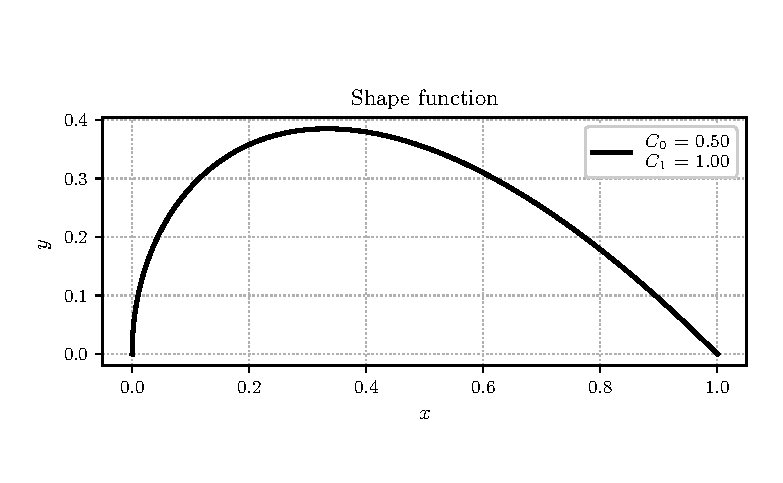
\includegraphics[width=\textwidth]{./images/class.eps}
        \end{figure}
    \end{columns}
\end{frame}

\begin{frame}{Blades - \Romannum{1}}
    % \vspace{1cm}
    \begin{figure}
        \hspace*{-0.8cm}
        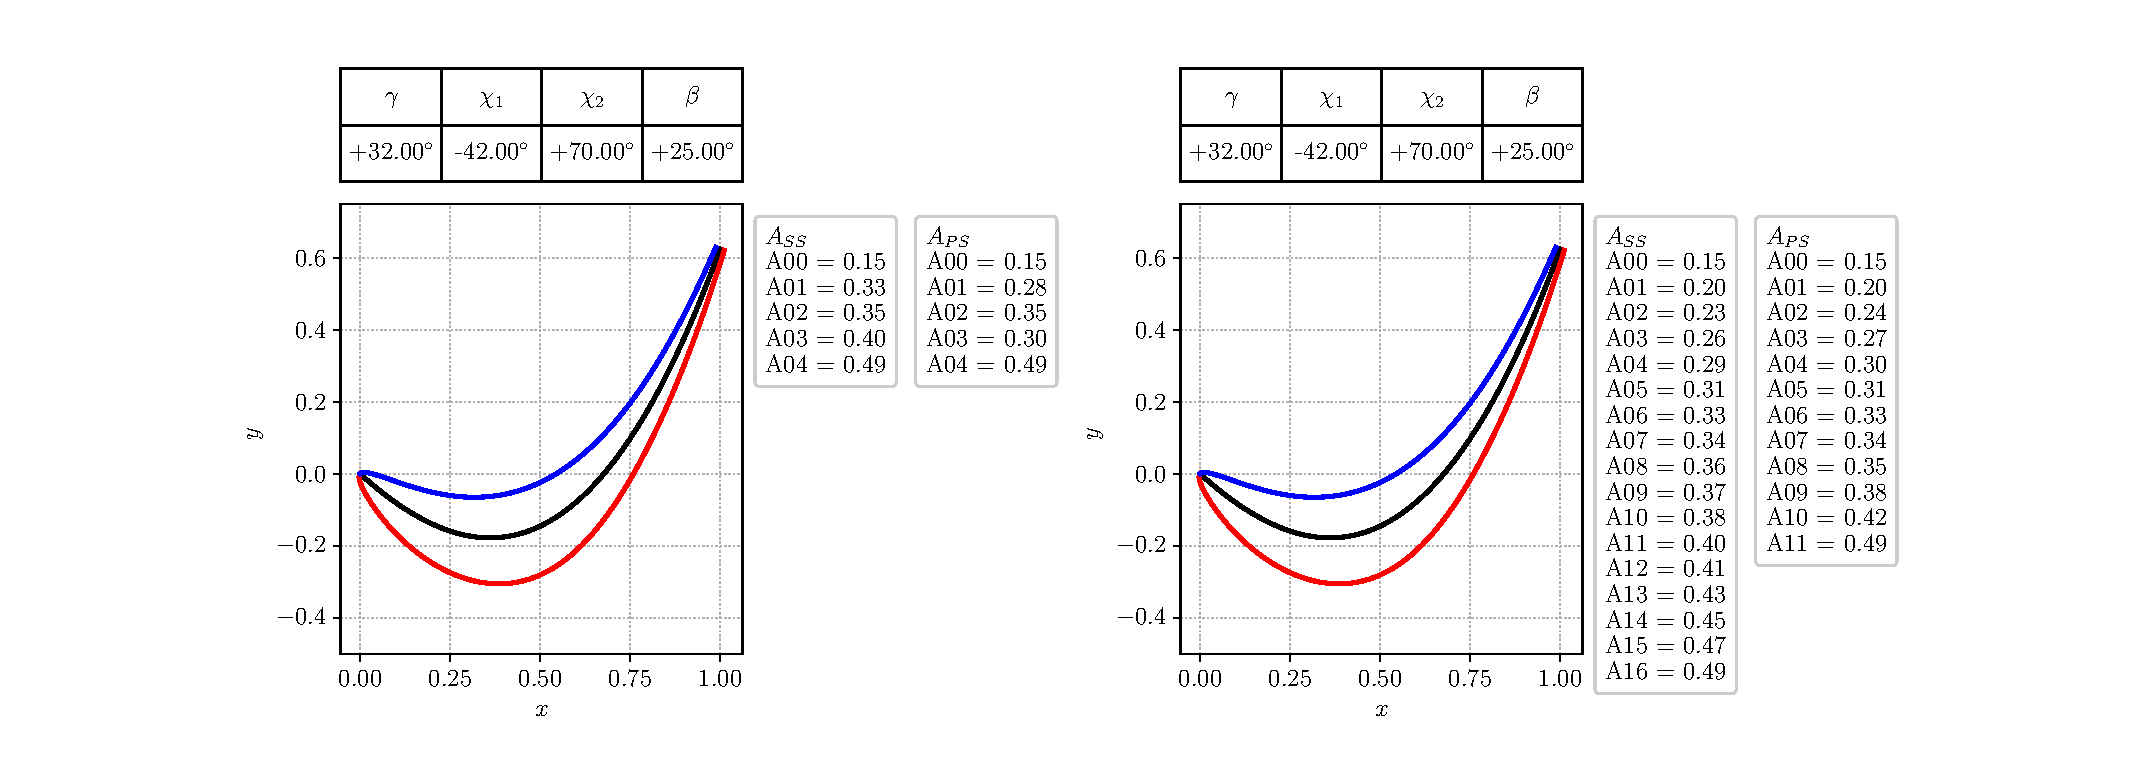
\includegraphics[width=1.2\textwidth, trim=3cm 0cm 0cm 0cm, clip]{./images/blade1.eps}
    \end{figure}
\end{frame}

\begin{frame}{Blades - \Romannum{2}}
    \begin{figure}
        \hspace*{-0.8cm}
        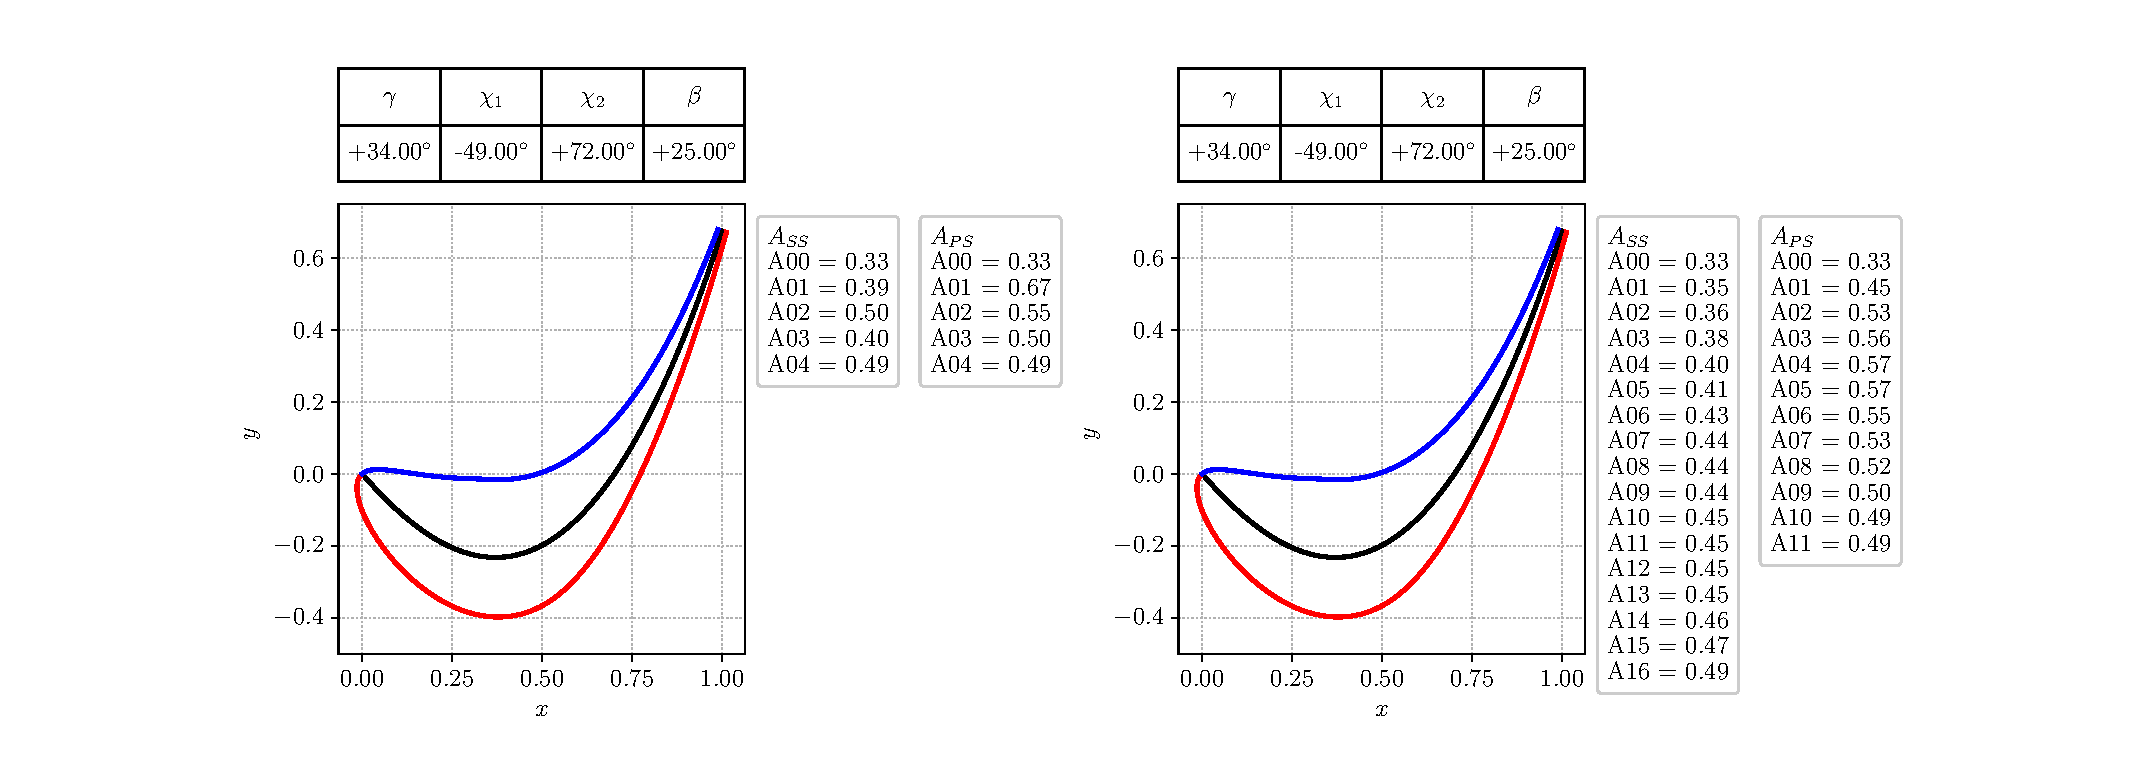
\includegraphics[width=1.2\textwidth, trim=3cm 0cm 0cm 0cm, clip]{./images/blade2.eps}
    \end{figure}
\end{frame}

% \begin{frame}{Kulfan thickness functions}
%     Kulfan thickness distribution is computed using $C_{(x)}$ and $S_{(x, i, N)}$:
%     \begin{equation}
%         \zeta_{(x)} = \sum_{i = 0}^N S_{(x, i, N)} \cdot C_{(x)} \notag
%     \end{equation}
%     \vspace{-2cm}
%     \begin{figure}
%         % 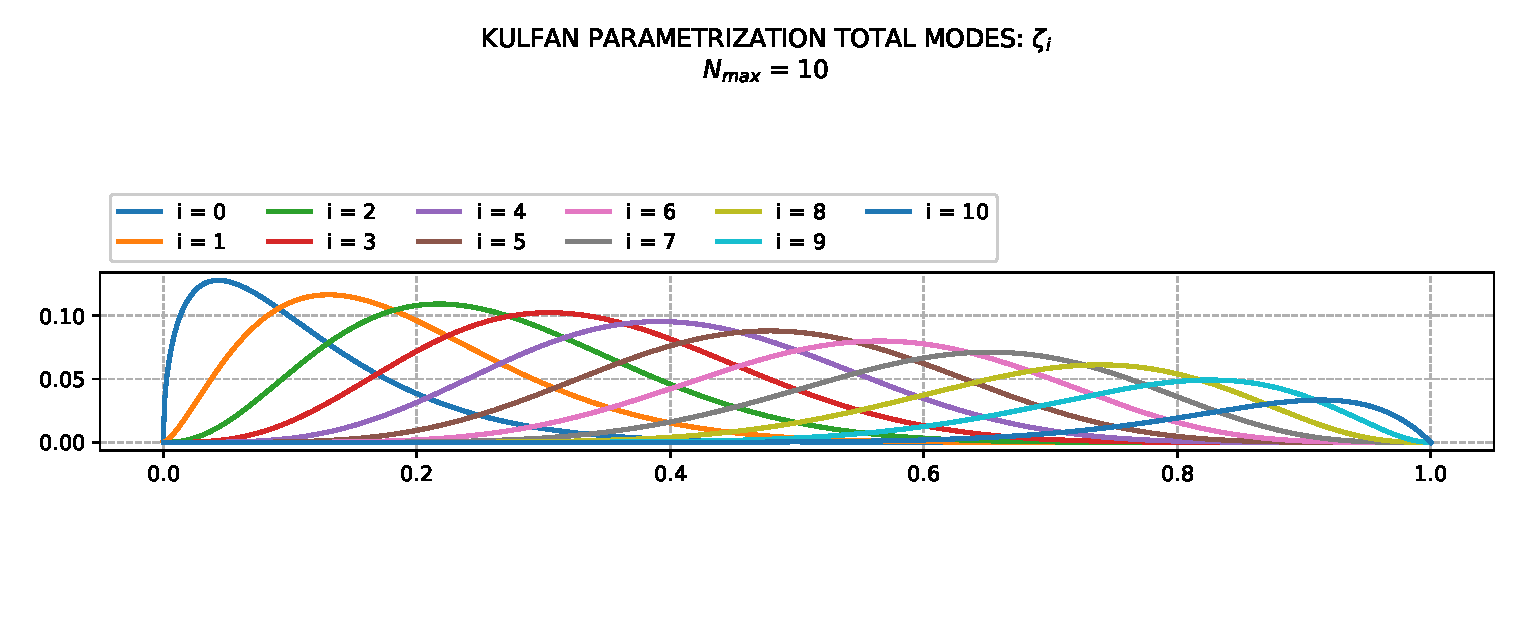
\includegraphics[width=\textwidth]{images/profileLine/kulfan.eps}
%         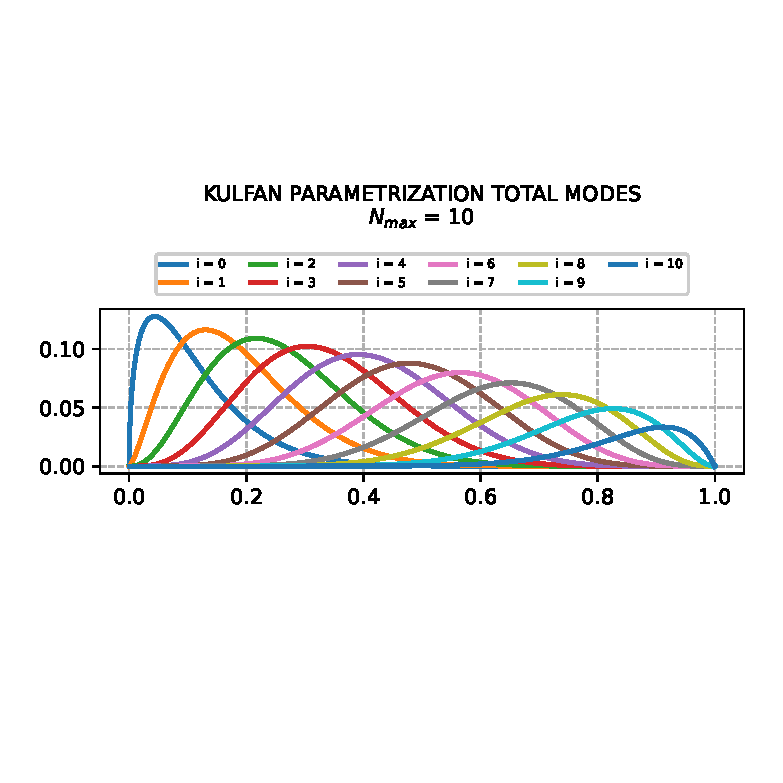
\includegraphics[scale=0.8]{./images/kulfanFunction.eps}
%     \end{figure}
% \end{frame}

% \begin{frame}{Thickness distribution and scaling}
%     \begin{block}{Pressure/suction side generation $(\pm)$}
%         \vspace*{-0.6cm}
%         \begin{align*}
%             \zeta_{TOT_{(x)}} & = \zeta_{(x)} + \zeta_{TE} \cdot x \\
%             x_{PS/SS}         & = x_{camberline} \pm n_x \cdot \zeta_{TOT_{(x)}} \cdot S_{(x, 0, 2)} \\ 
%             y_{PS/SS}         & = y_{camberline} \pm n_y \cdot \zeta_{TOT_{(x)}} \cdot S_{(x, 0, 2)} + \zeta_{(x)} \cdot \big[1 - S_{(x, 0, 2)}\big]
%         \end{align*}
%     \end{block}
%     \vspace{-0.9cm}
%     \begin{columns}
%         \column{0.5\textwidth}
%             \begin{figure}
%                 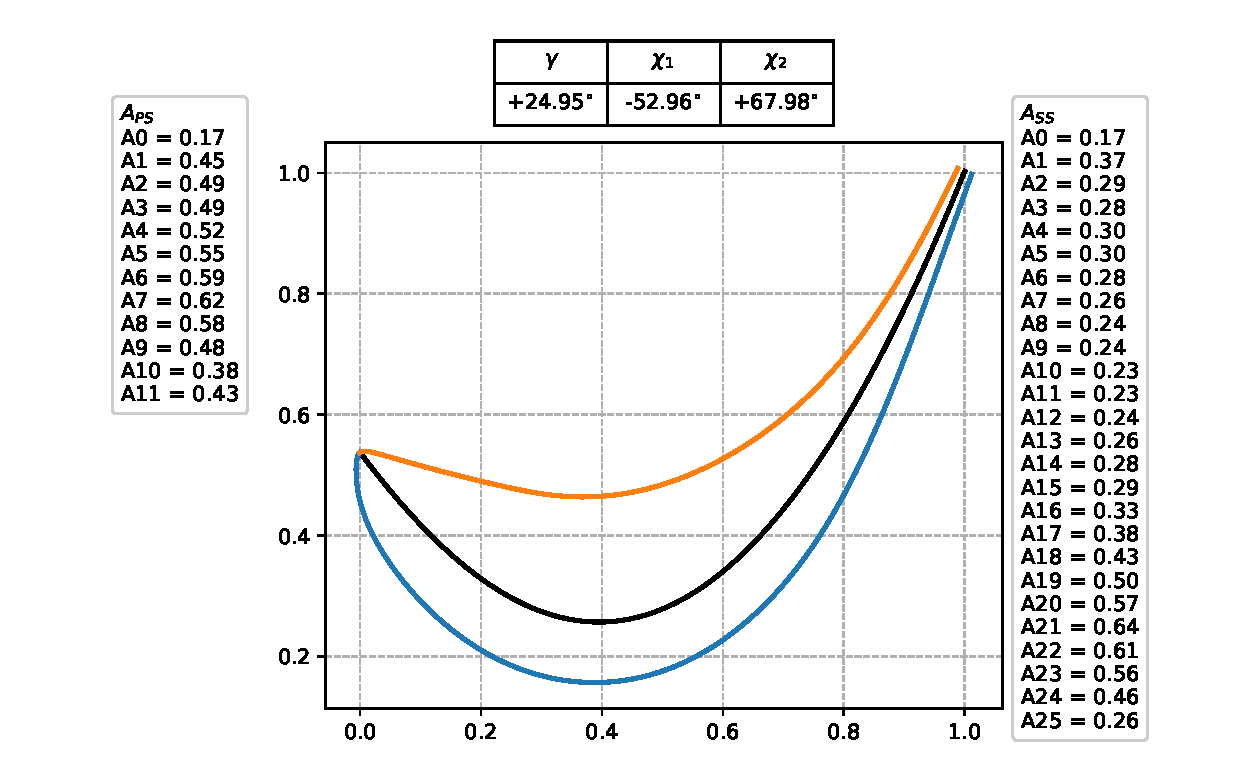
\includegraphics[width=\textwidth]{images/profileLine/blade01.eps}
%             \end{figure}
%         \column{0.5\textwidth}
%             \begin{figure}
%                 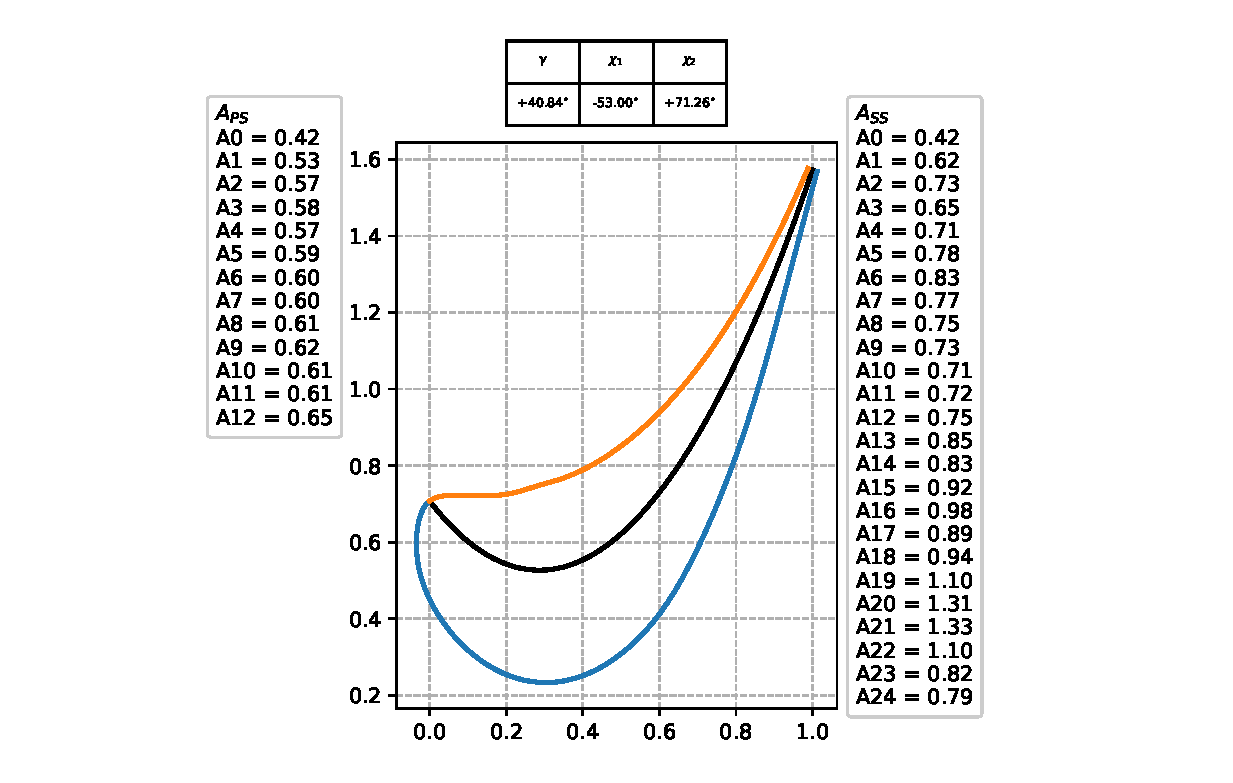
\includegraphics[width=\textwidth]{images/profileLine/blade02.eps}
%             \end{figure}
%     \end{columns}
% \end{frame}

\subsection{Aerodynamic Duty}
\SubSectionPage

\begin{figure}[!h]

    \begin{center} 
    
        \begin{tikzpicture}
            \begin{axis}[
                width=0.5\textwidth, % Increased width
                axis equal,          % Set equal aspect ratio
                axis lines=none,     % Remove axis lines and labels
                xmin=-0.3, xmax=1.3, % Increased x limits
                ymin=-0.1, ymax=1.6,   % Increased y limits
            ]

            \addplot[black, line width=2pt] table[x index=0, y index=1, col sep=comma] {./pyFigure/csv/coords.csv};
            \addplot[black, line width=2pt] table[x index=2, y index=3, col sep=comma] {./pyFigure/csv/coords.csv};
            
            % Adding the second arrow with text
            \draw[-latex, line width=2.5pt] (axis cs:-0.25,0.55) -- node[below left] {$Re$} (axis cs:-0.05,0.35);
            \draw[-latex, line width=2.5pt] (axis cs:1.02,1) -- node[above left] {$M_2$} (axis cs:1.22,1.6);
            \draw[-, line width=1.0pt] (axis cs:-0.25,0.55) -- node[below] {$\alpha_1$} (axis cs:0.15, 0.55);
            \draw[-, line width=1.0pt] (axis cs:1.02,1) -- node[above left] {$\alpha_2$} (axis cs:1.45, 1);
            
            \end{axis}
        \end{tikzpicture}
    
    \end{center}

    \caption{Aerodynamic duty parameters.}
    \label{fig:aeroDuty}

\end{figure}

\subsection{Aerodynamic Style}
\SubSectionPage

\begin{frame}{Aerodynamic Style}
    The aerodynamic style is a way for defining the \textbf{load distribution} (in this case in terms of the Mach number fraction $\frac{M}{M_{TE}}$) over the blade.
    \begin{columns}
        \column{0.53\textwidth}
        \begin{block}{System objectives}
            \begin{itemize}
                \setlength\itemsep{0.3cm}
                \item $\frac{M_P}{M_{TE}}$: peak Mach fraction
                \item $\frac{L_P}{L_{surf}}$: peak surface fraction
                \item $\frac{M_{LE}}{M_{TE}}\frac{M_2}{M_1}$: leading edge Mach fraction
                \item $\frac{M_{PS}}{M_{TE}}\frac{M_2}{M_{1, ax}}$: pressure side Mach fraction
            \end{itemize}
        \end{block}
        \column{0.52\textwidth}
            \vspace{-2cm}
            \begin{figure}
                \centering
                \animategraphics[autoplay,loop,controls=off,width=8cm,height=8cm]{10}{gif/aeroStyle}{0}{99}
            \end{figure}
    \end{columns}
\end{frame}

\section{Database Generation}
\SectionPage

\begin{frame}{Steps}
    \vspace{-1.5cm}
    \begin{figure}
        \vspace{0.5cm}
        \centering
            \begin{tikzpicture}[
                mindmap,
                every node/.style=concept,
                concept color=black!20,
                grow cyclic,
                level 1/.append style={level distance=8cm, sibling angle=40, font=\small},
                level 2/.append style={level distance=5cm, sibling angle=27, font=\small}
                ]
                \node [root concept, scale=0.85] {{\LARGE\textbf{Data-Driven Design}}} % root
                    child [concept color=yellow!10, scale=0.5] { node (c1) {\textbf{Machine \\ Learning}}
                        child [rotate=40] { node [scale=0.6] {\textbf{PCA}} }
                        child [rotate=40] { node [scale=0.6] {\textbf{RBF}} }
                    }
                    child [concept color=orange, scale=0.5] { node [level distance=9cm] (c2) {\textbf{Database \\ Generation}} 
                        child [level distance=6cm] { node [scale=0.6, distance=10cm] {\textbf{Strategy}} }
                        child [level distance=6cm] { node [scale=0.6, distance=10cm] {\textbf{Flow Solver}} }
                        child [level distance=6cm] { node [scale=0.6, distance=10cm] {\textbf{Optimizer}} }
                    }
                    child [concept color=red!10, scale=0.5] { node (c3) {\textbf{Data \\ Setup}}
                    child [rotate=-30] { node [scale = 0.6] {\textbf{Style}} }
                    child [rotate=-30] { node [scale = 0.6] {\textbf{Duty}} }
                    child [rotate=-30] { node [scale = 0.6] {\textbf{Blade}} } 
                    };
                \begin{pgfonlayer}{background}
                    \draw [concept connection]  (c1) edge (c2)
                                                     edge (c3)
                                                (c2) edge (c3);
                    \end{pgfonlayer}
            \end{tikzpicture}
    \end{figure}
\end{frame}

\subsection{Flow Solver}
\SubSectionPage

\begin{frame}{Flow solver}
    \texttt{MISES} is based on a \textbf{Newton's method optimizer}. Giving geometry and constraints, the solver computes the blade channel flow. 
    % \\ [0.5cm]
    The solver relies on:
    \begin{align*}
        \text{\textbf{Momentum equation}: }\mathcal{R}_1 & = \Delta p + \frac{m}{A} \Delta \tilde{q} - P_s - p \ \Delta \mathcal{P} = 0 \\
        \text{\textbf{Entropy equation}: }\mathcal{R}_2 & = p \ \Delta \log{\tilde{p}_{0, a}} - p \ \Delta \mathcal{P} = 0
    \end{align*}
    These 2 models are \textbf{blended} into one single equation:
    \begin{equation*}
        \mathnormal{g} \cdot \mathcal{R}_1 + (1 - \mathnormal{g}) \cdot \mathcal{R}_2 = 0
    \end{equation*}
    Where $\mathnormal{g}$ takes into account the local changes of \textbf{total pressure} and the \textbf{velocity gradients}.
    \\ [0.5cm]
    The solver models the boundary layer using \textbf{interchangeably} the $\boldsymbol{e^n}$ and \textbf{Abu-Ghannam-Shaw} models.
\end{frame}

\begin{frame}{\texttt{MISES} - Geometry, BCs \& control points}
    \vspace{-3cm}
    \begin{columns}
        \column{0.5\textwidth}
        \vspace{2cm}
        \begin{figure}
            \centering
            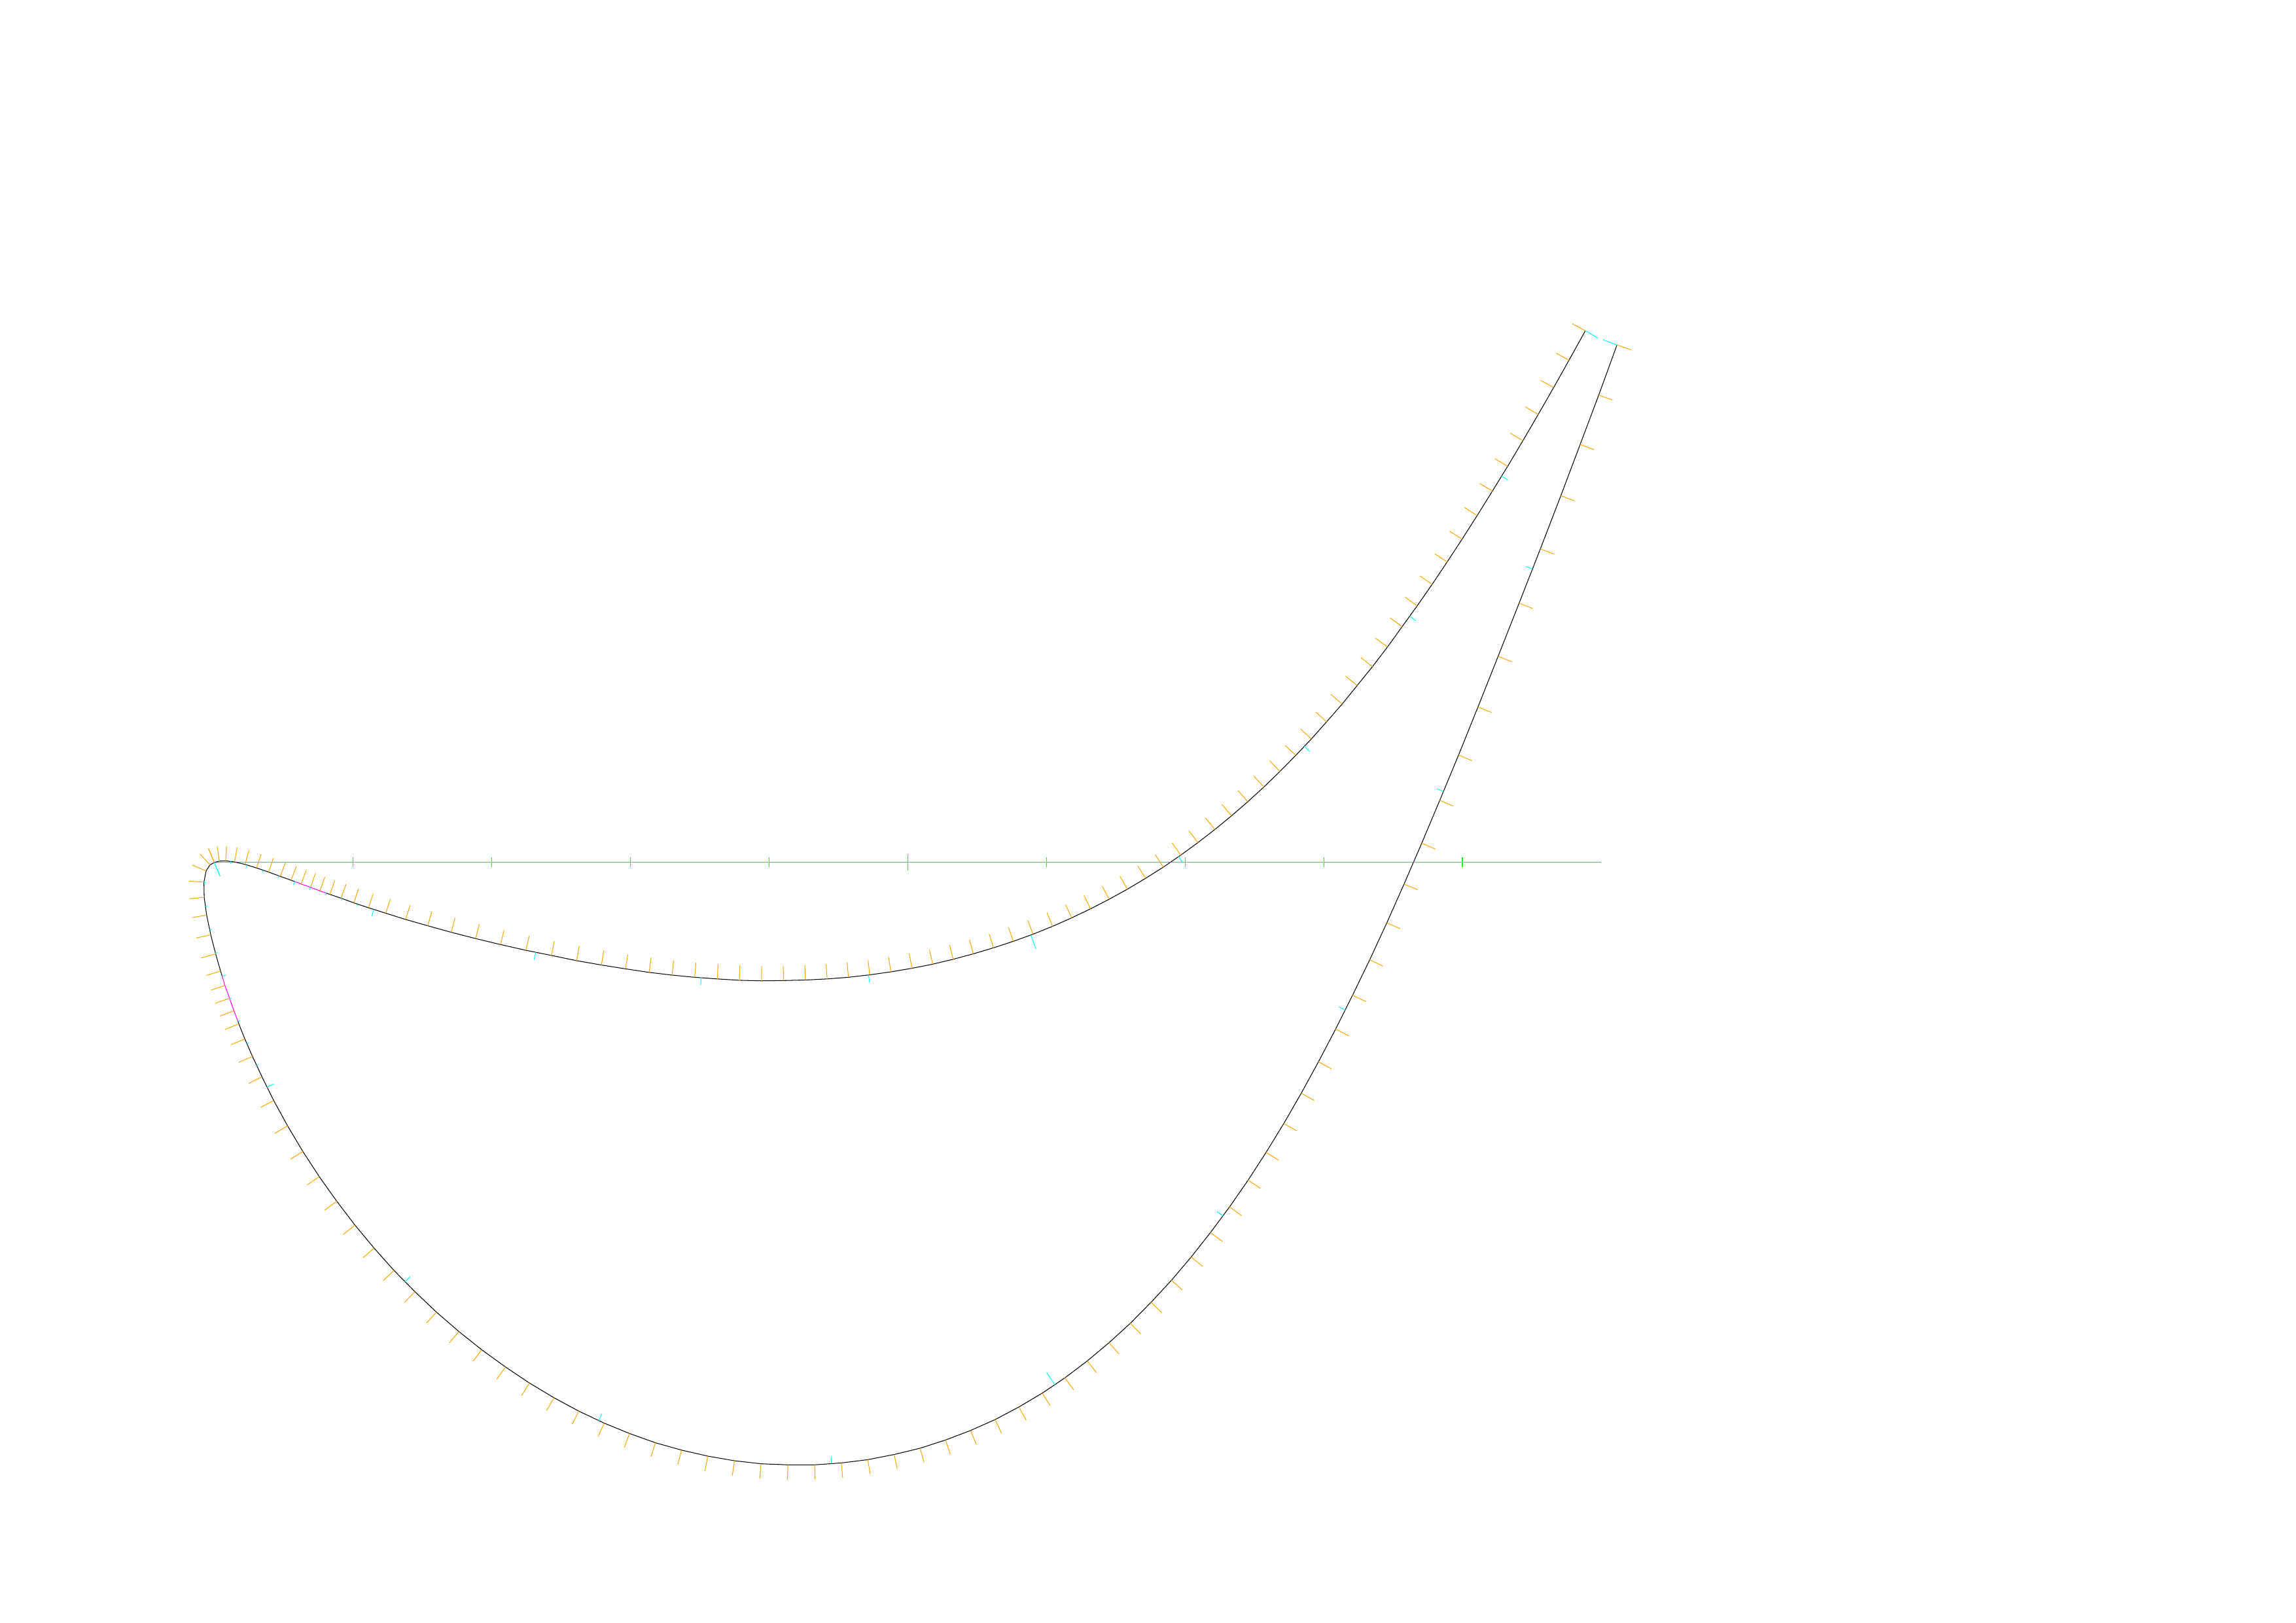
\includegraphics[scale=0.3]{./images/datablade120-2.png}
        \end{figure}
        \column{0.5\textwidth}
        \begin{figure}
            \centering
            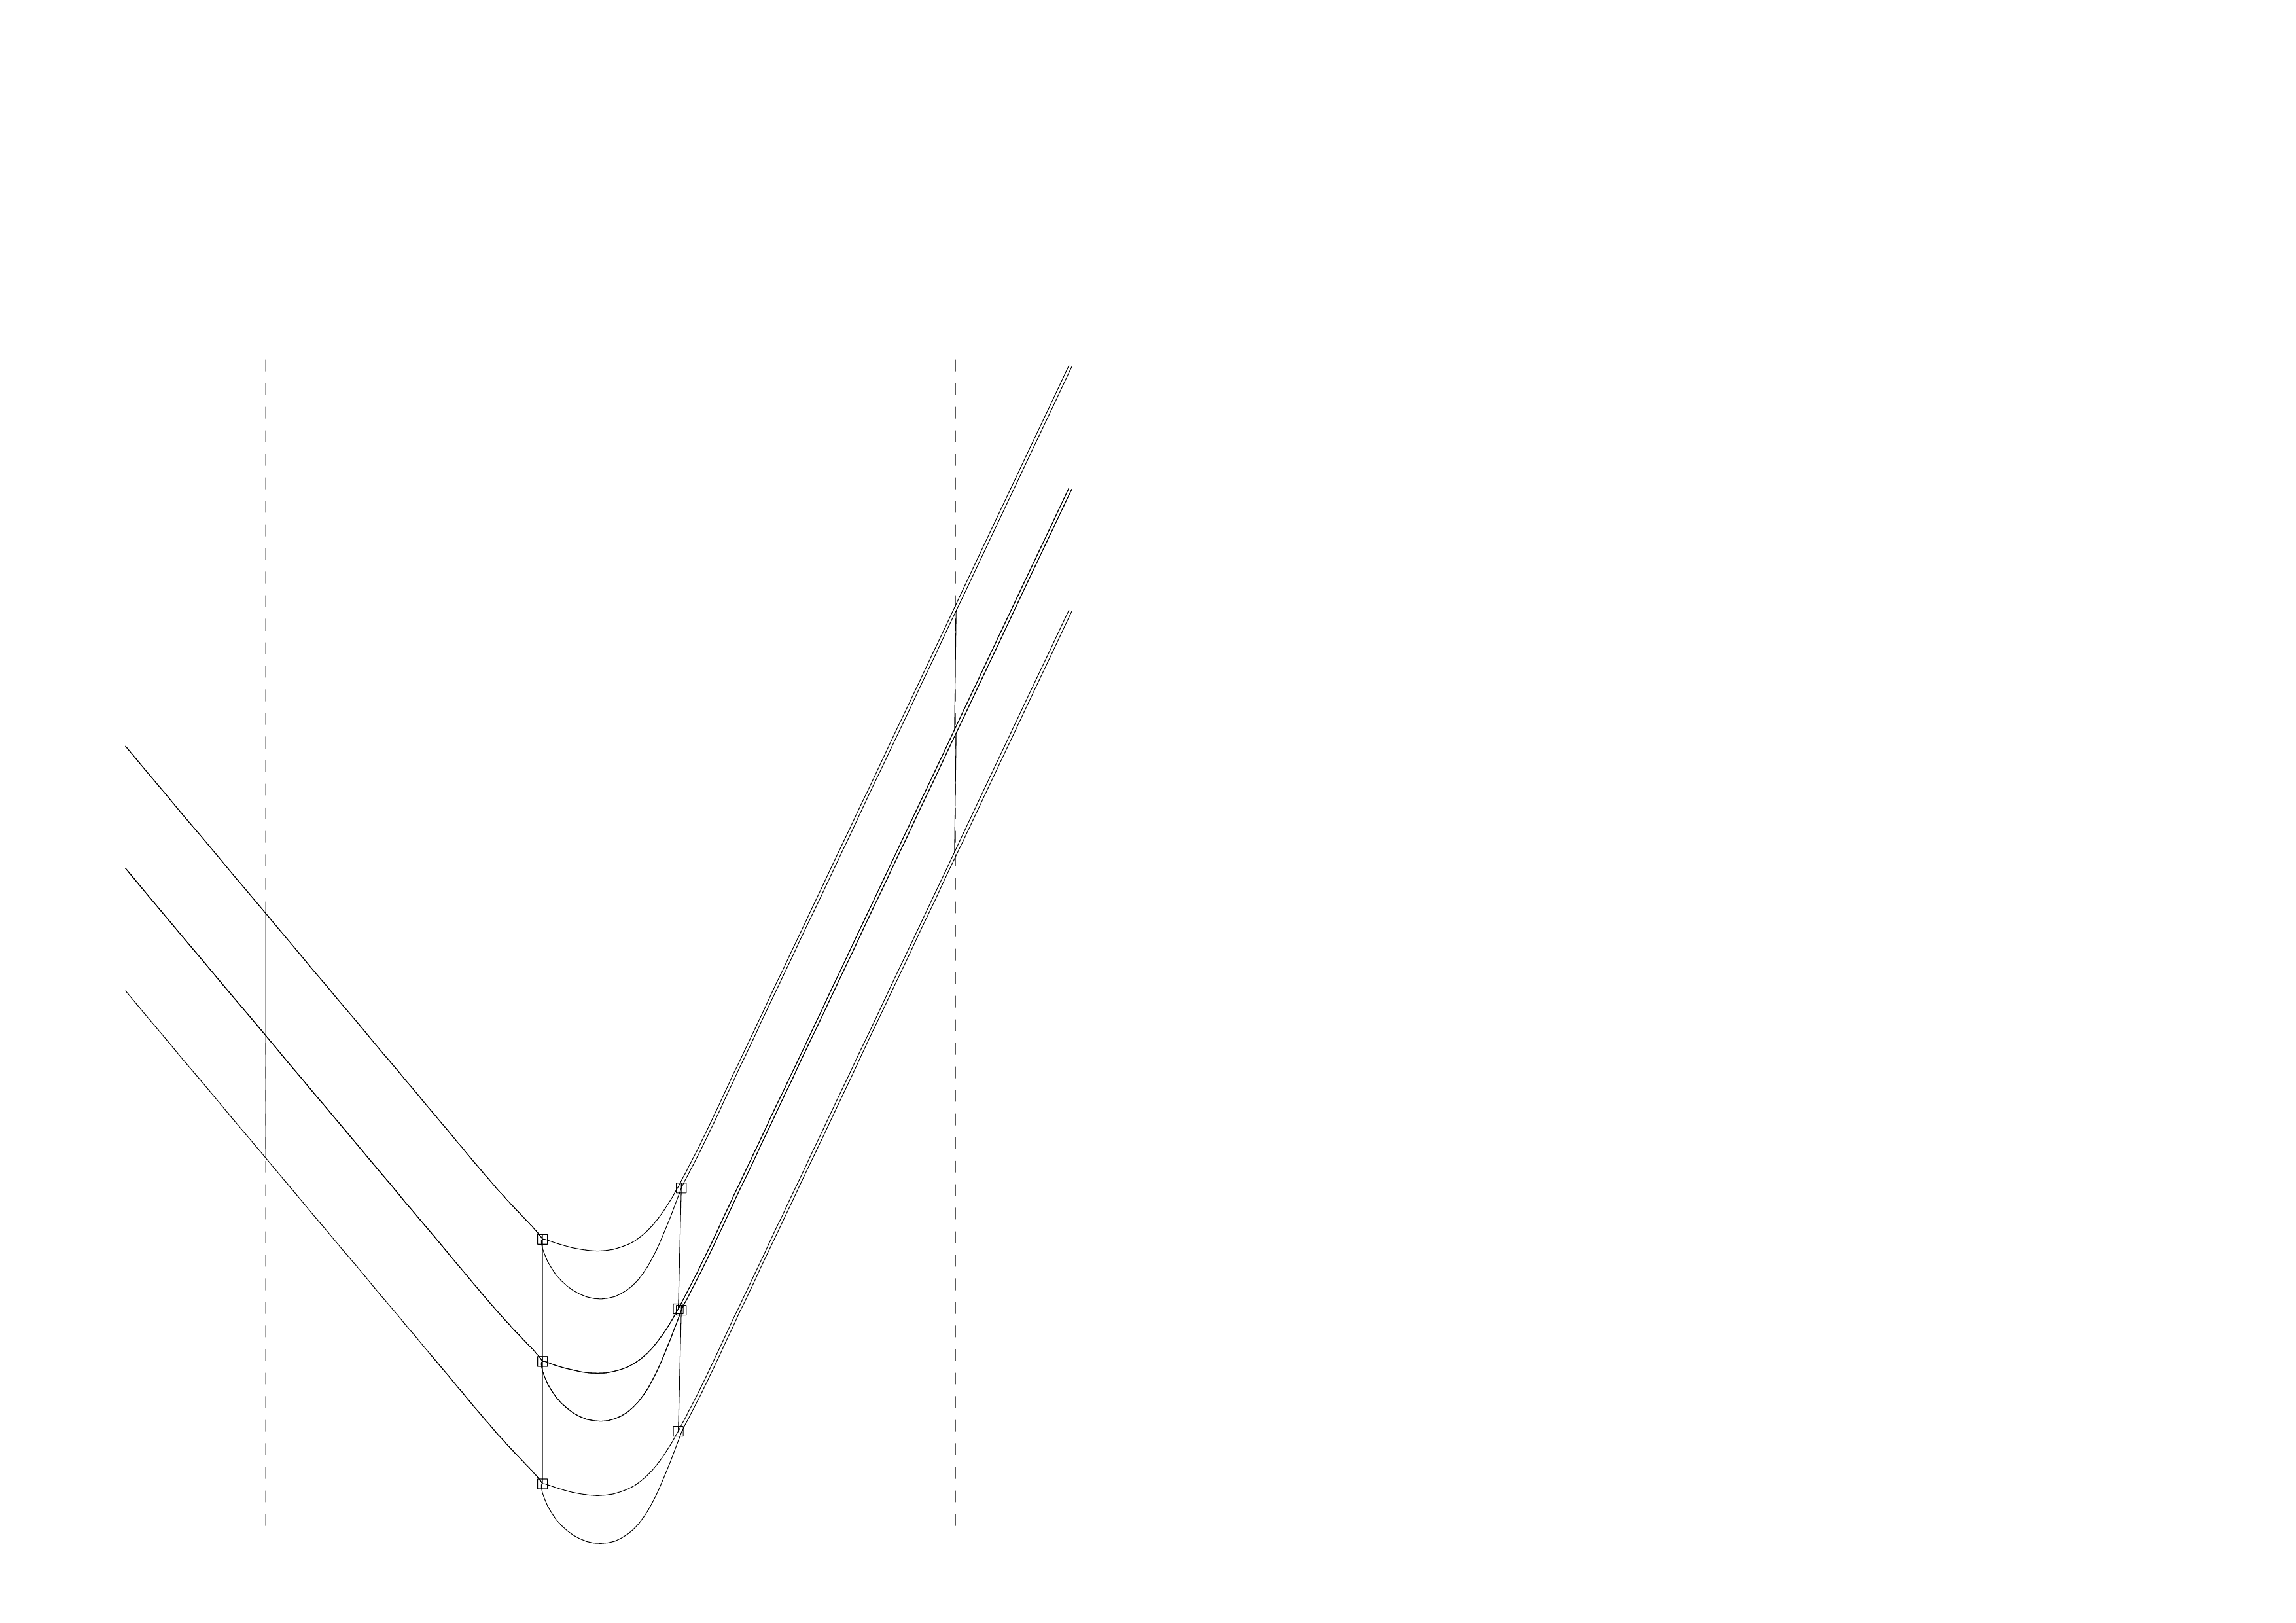
\includegraphics[scale=0.4]{./images/datablade120-1.png}
        \end{figure}
    \end{columns}
\end{frame}

\begin{frame}{\texttt{MISES} - Grid \& flow}
    \vspace{-2.5cm}
    \begin{columns}
        \column{0.5\textwidth}
        \vspace{0.5cm}
        \begin{figure}
            \centering
            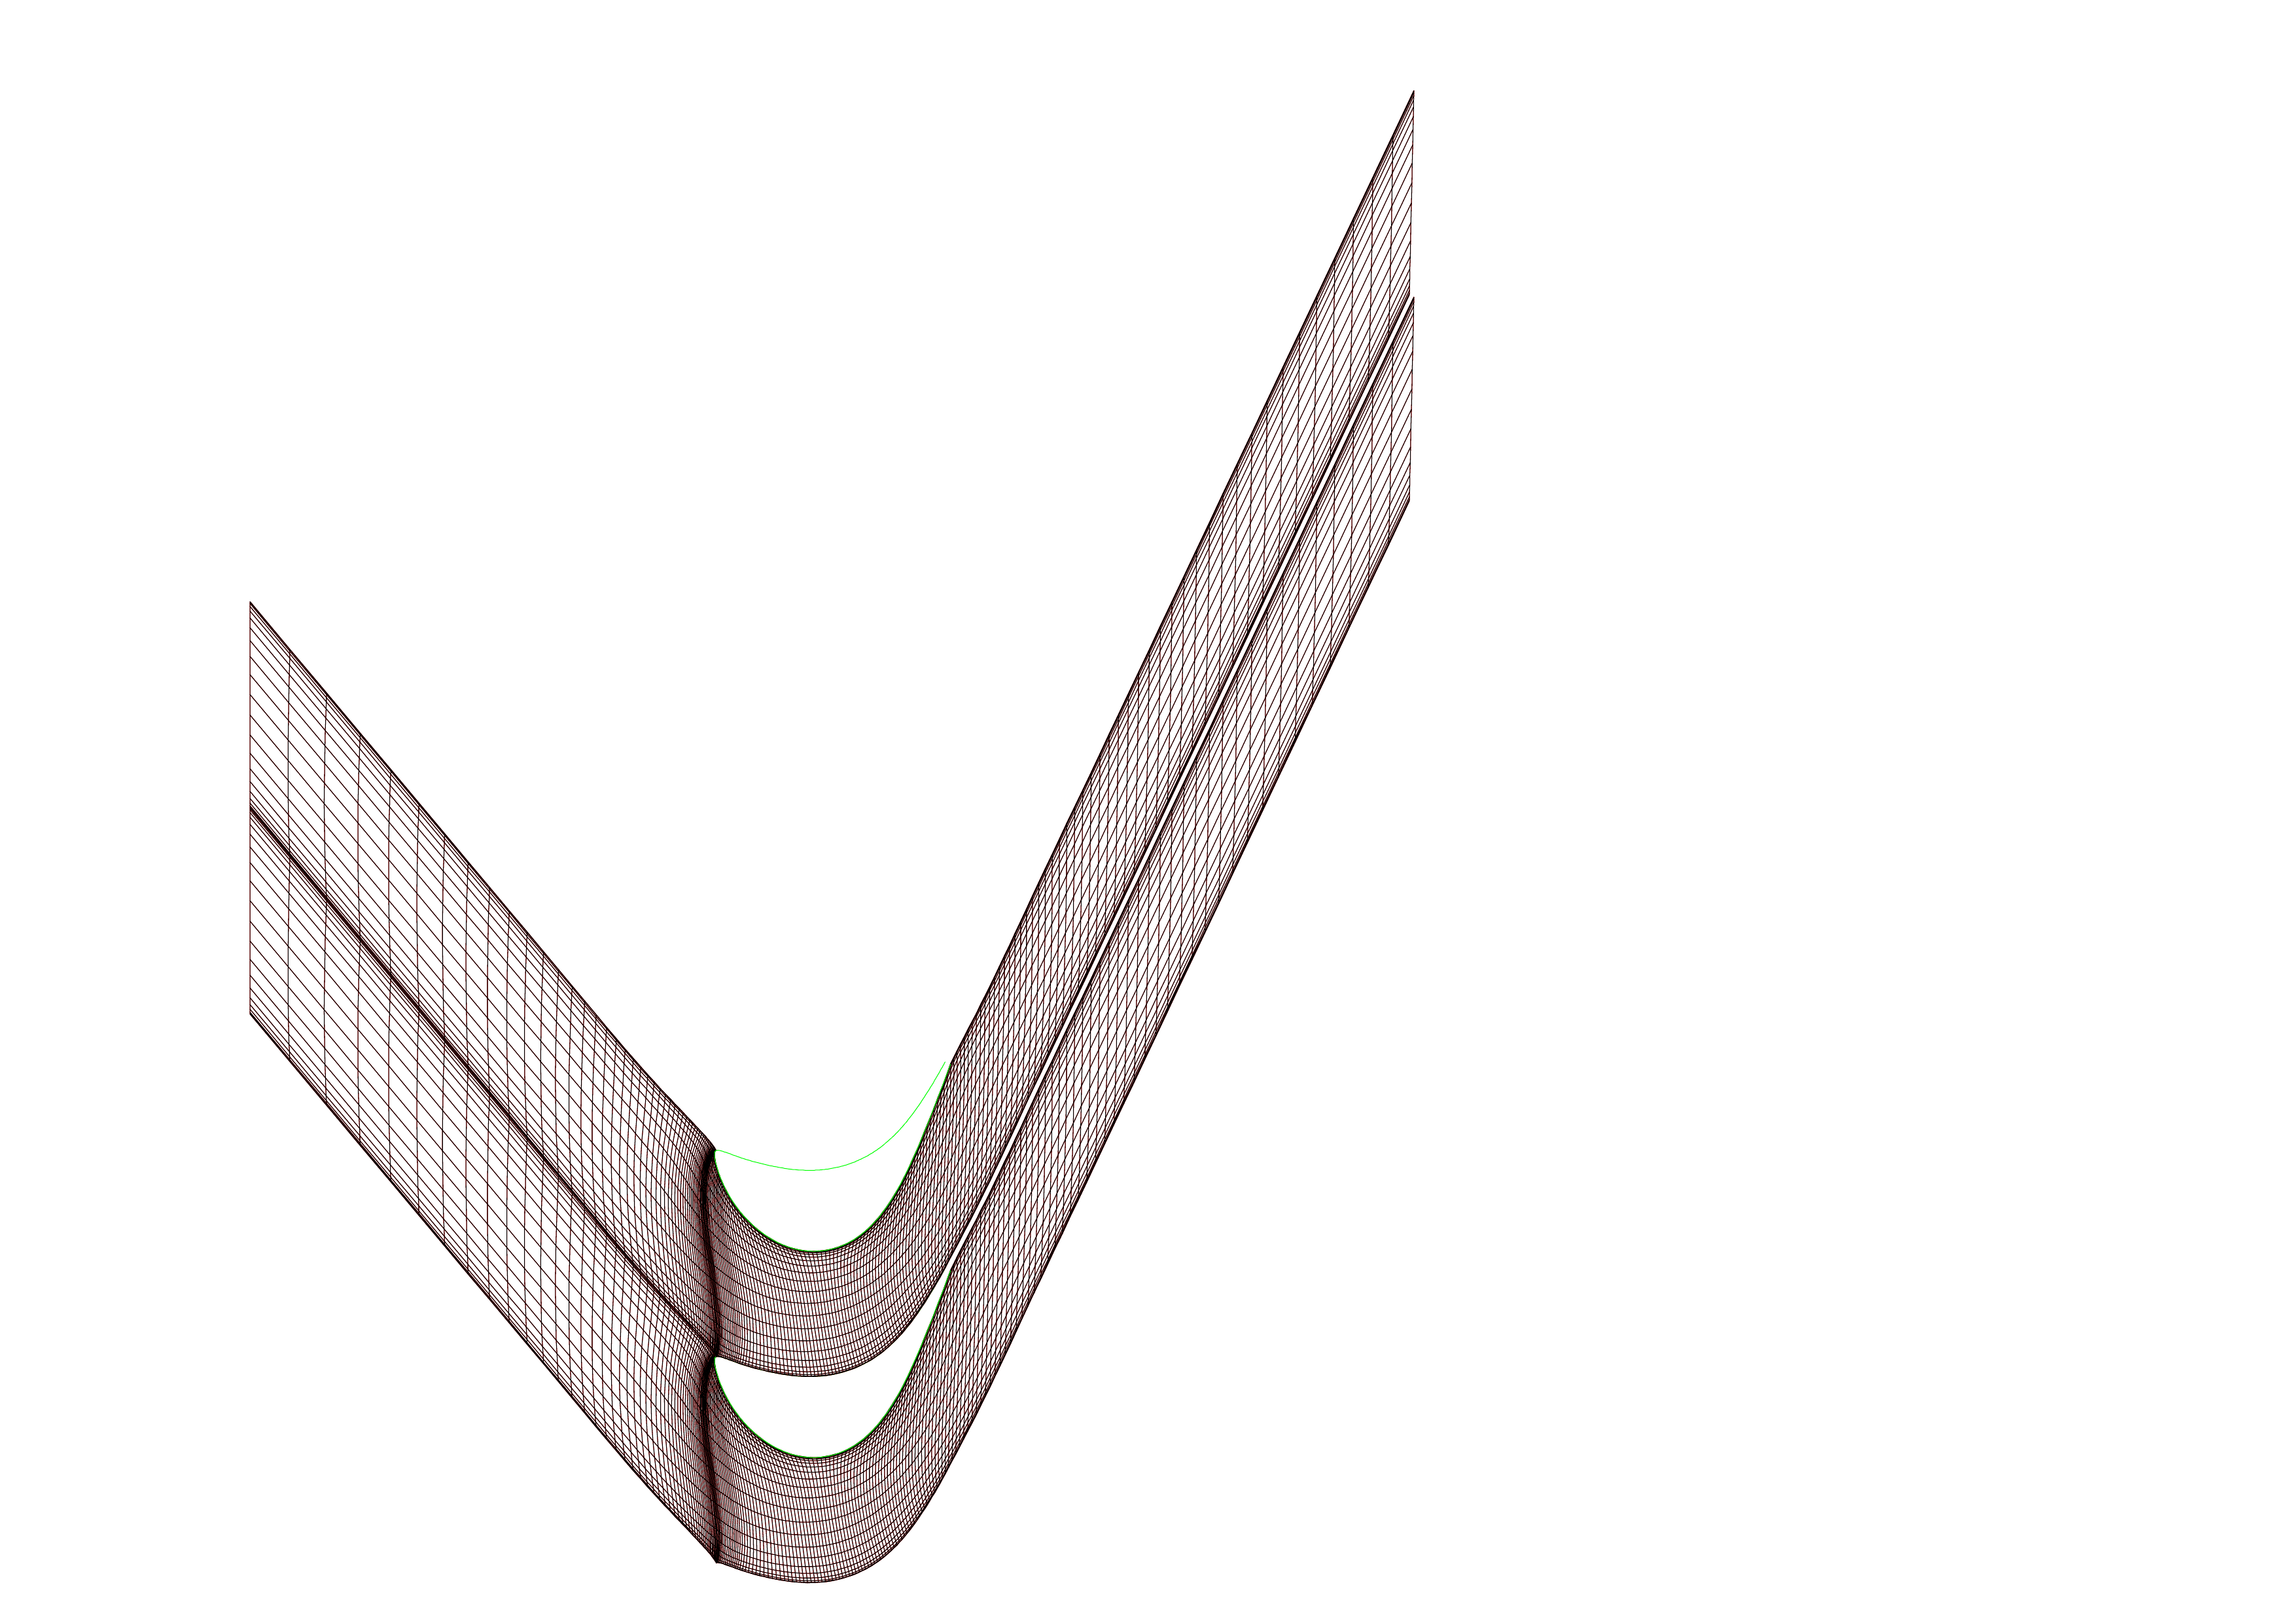
\includegraphics[scale=0.4]{./images/datablade120-3.png}
        \end{figure}
        \column{0.5\textwidth}
        \begin{figure}
            \centering
            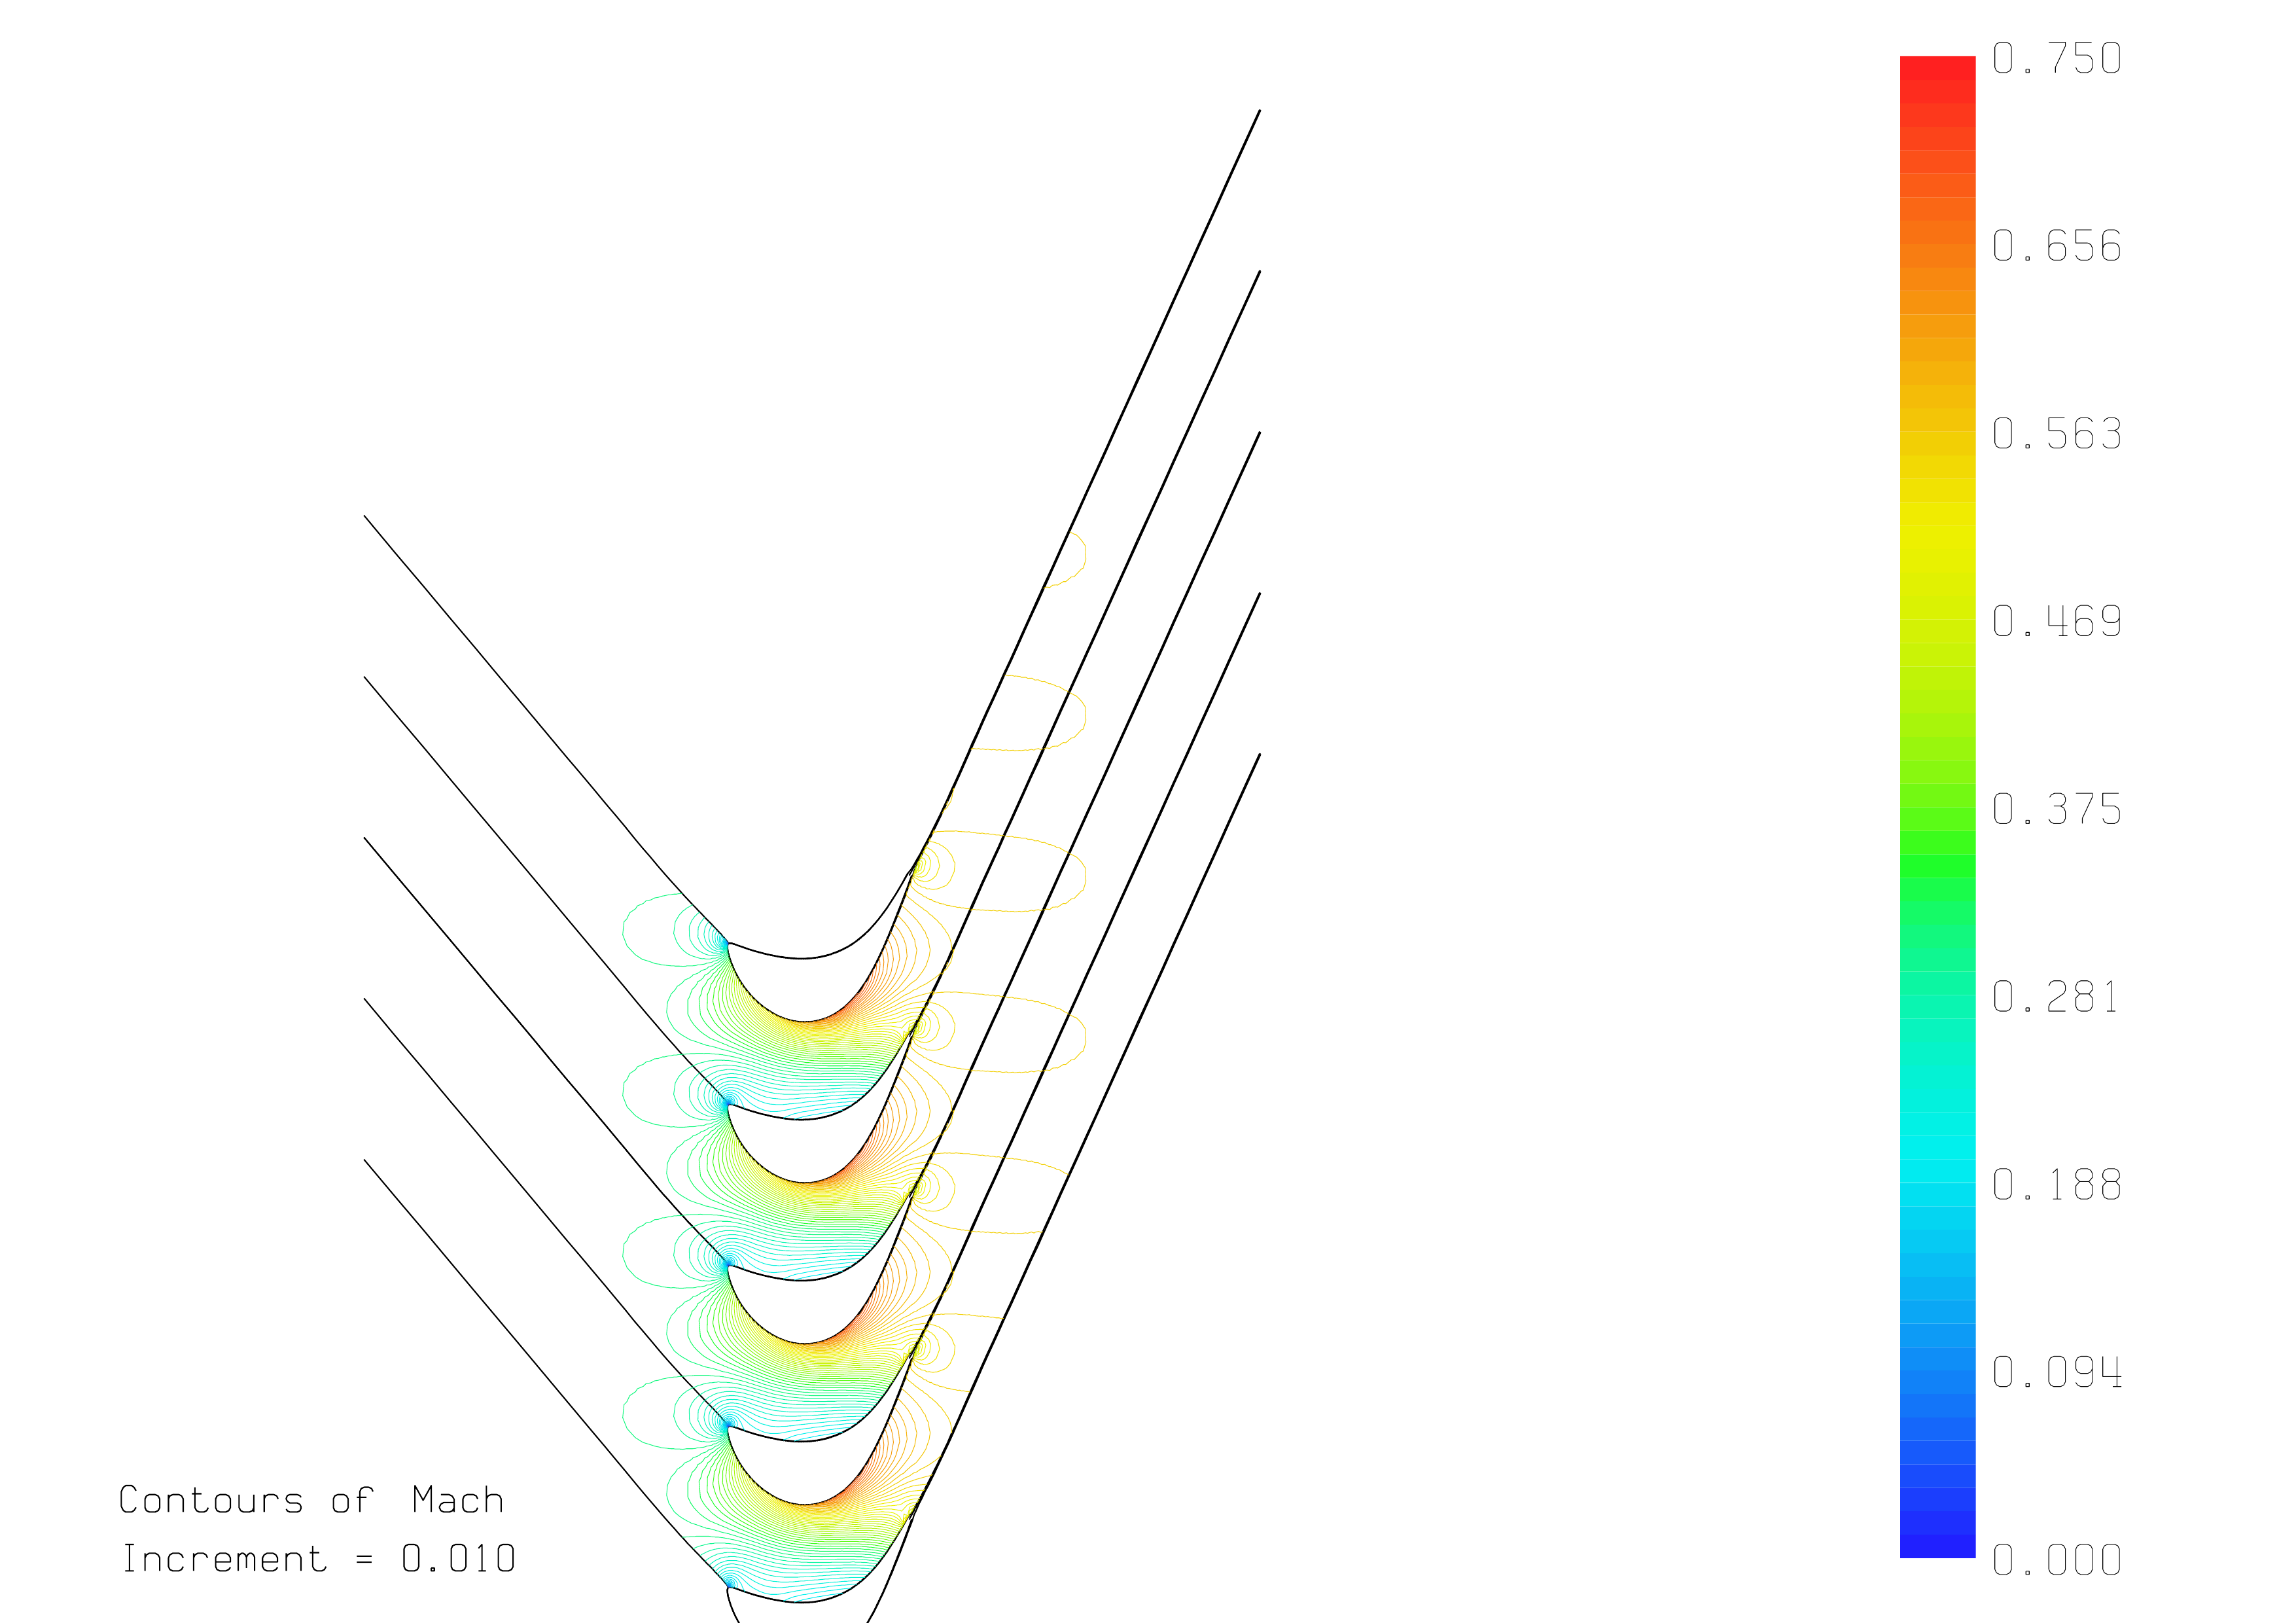
\includegraphics[scale=0.4]{./images/datablade120-4.png}
        \end{figure}
    \end{columns}
\end{frame}

% \begin{frame}{\texttt{MISES} Input -- Setup}
%     \begin{block}{Inputs}
%         \begin{itemize}
%         \item Flow properties:
%         \begin{itemize}
%             \item \texttt{MOUT = } $ M_2$: mixed outlet Mach flow
%             \item \texttt{SINL = } $\tan(\alpha_{1})$: inlet flow angle slope
%         \end{itemize}
%         \item Grid properties:
%         \begin{itemize}     
%             \item \texttt{F F}: grid setup, \texttt{H-type} grid for the inlet, the blade-to-blade plane and the outlet of the mesh
%         \end{itemize}
%         \item Turbulence:
%         \begin{itemize}
%             \item \texttt{REYin = } $Re = 6 \cdot 10^5$: flow Reynolds number
%             \item \texttt{NCRIT = } $n_{crit} = 4$: turbulence model parameter following Abu-Ghannam-Shaw model
%             \item \texttt{XTR1 = XTR2 = } $0.15$: imposed turbulence transition point over the blade
%         \end{itemize}
%     \end{itemize}
%     \end{block}
% \end{frame}

% \begin{frame}{\texttt{MISES} Input -- Properties}
%     \begin{alertblock}{Grid properties and test}
%         After many tests comparing \texttt{H-type} grid with \texttt{I-type} grid. The \texttt{H-type} grid allows faster execution time for the flow computation with neglecting difference on the flow output to \texttt{I-type} based simulations. This because shock waves are not present inside the domain.
%     \end{alertblock}
%     \begin{alertblock}{Turbulence properties}
%         \begin{itemize}
%             \item The $n_{crit}$ parameter has been chosen looking at a \texttt{MISES} input file for a turbine blade that sits in the working range conditions.
%             \item During the simulation, the turbulence model will then adapt the transition points to the most physical positions on the blade. This number is setup for reducing simulation convergence steps.
%         \end{itemize}
%     \end{alertblock}
% \end{frame}

% \begin{frame}{\texttt{MISES} simulation}
%     \begin{block}{Simulation}
%         \begin{itemize}
%             \item \texttt{ISMOM = 4}: this is the setup to attack the problem. The flow is studied as isentropic in the whole system except where shocks are present (which in this range of study are not so common). The switch from one solver to another is dictate by the $\rho$ field.
%             \item Log files are generated after each simulation for convergence tracking and flow properties study.
%             \item Computation of the Mach distribution over the blade.
%         \end{itemize}
%     \end{block}
% \end{frame}

% \hidelogo
% \begin{frame}{Postprocessing}
%     \begin{alertblock}{Load error computation}
%         The steps followed for the error computation on the aerodynamic load are:
%         \begin{itemize}
%             \item \texttt{MISES} computation
%             \item \texttt{MISES} call that generated Mach distribution over the blade
%             \item Reading of the Mach distribution file getting Mach curve and $M_{TE}$ for the Mach fraction generation
%             \item Computation of the RMSE error using the aerodynamic style target and the Mach fraction load converted in surface fraction. 
%             \item Cost computation 
%         \end{itemize}
%     \end{alertblock}
% \end{frame}
% \begin{frame}{Cost Function}
%     The cost function for the optimization of the blade is:
%     \begin{align*}
%         \Delta \alpha_2 & = | \alpha_{2, \texttt{MISES}} - \alpha_2 | \\ 
%         cost            & = RMSE \cdot \big[1 + 0.01 \cdot \big( 2 \cdot max(0, \Delta \alpha_{2} - \alpha_{th}) \big)^2 \big] \notag
%     \end{align*}
%     \begin{itemize}
%         \item The cost function allows to reduce the outlet flow angle error and the error on the load distribution at the same time. 
%         \item $\Delta \alpha_2$ is the absolute value of the error over the exit flow angle.
%         \item The $\alpha_{th}$ value is a threshold on the outlet flow error.
%     \end{itemize}
% \end{frame}



\subsection{Optimization in Turbine Design Process}
\SubSectionPage

\begin{frame}{Database generation strategy}
    \newcommand\WIDTH{3.5cm}
    \newcommand\HEIGHT{1.5cm}
    \newcommand\Ydist{2cm}
    \newcommand\XPOS{4cm}
    \newcommand\TOTheight{5cm}
    \newcommand\TOTwidth{6cm}
    \newcommand\PTS{2pt}
    \newcommand\xSpace{0.5cm}

    \only<1>{
        \begin{figure}
            \centering
            \vspace*{0.5cm}
            \hspace*{0.3cm}
            \begin{tikzpicture}
    
    \node[draw,
        rectangle,
        text centered,
        line width = \PTS,
        minimum height = \TOTheight,
        minimum width = \TOTwidth
    ] (optimizationProcess) at (0, 0) {\large{\textbf{Optimization}}};

    % \node[
    %     below right = 0.5cm and 0.5cm of optimizationProcess.north west 
    % ] {
    %     
\includegraphics[scale=0.08]{./MITlogo.png}
    % };

    % \node[
    %     above left = 0.15cm and 0.5cm of optimizationProcess.south east 
    % ] {
    %     
\includegraphics[scale=0.3]{./SCIPYlogo.png}
    % };

    \node[draw,
        rectangle,
        text centered,
        line width = \PTS,
        % minimum width = \WIDTH,
        minimum height = \HEIGHT,
        right = 2*\xSpace of optimizationProcess
    ] (database) {\large{\textbf{Database}}};
    
    \coordinate[left=\xSpace of optimizationProcess.west]  (c1) {};
    \coordinate[above=\Ydist of c1]                      (c2) {};
    \coordinate[below=\Ydist of c1]                      (c3) {};

    \node[draw,
        rectangle,
        text centered,
        line width = \PTS,
        minimum width = \WIDTH,
        minimum height = \HEIGHT,
        left = \xSpace of c2
    ] (designSpace) {\large{\textbf{\makecell[c]{Design space\\reduction}}}};

    \node[draw,
        rectangle,
        text centered,
        line width = \PTS,
        minimum width = \WIDTH,
        minimum height = \HEIGHT,
        left = \xSpace of c1
    ] (constr) {\large{\textbf{Constraints}}};

    \node[draw,
        rectangle,
        text centered,
        line width = \PTS,
        minimum width = \WIDTH,
        minimum height = \HEIGHT,
        left = \xSpace of c3
    ] (obj) {\large{\textbf{Objectives}}};

    \draw[-latex, line width = 1pt] (designSpace) -- (c2) -- (c1) to (optimizationProcess.west);
    \draw[-latex, line width = 1pt] (constr) to (optimizationProcess.west);
    \draw[-latex, line width = 1pt] (obj) -- (c3) -- (c1) to (optimizationProcess.west);
    \draw[-latex, line width = 1pt] (optimizationProcess.east) to (database.west);

\end{tikzpicture}
            % 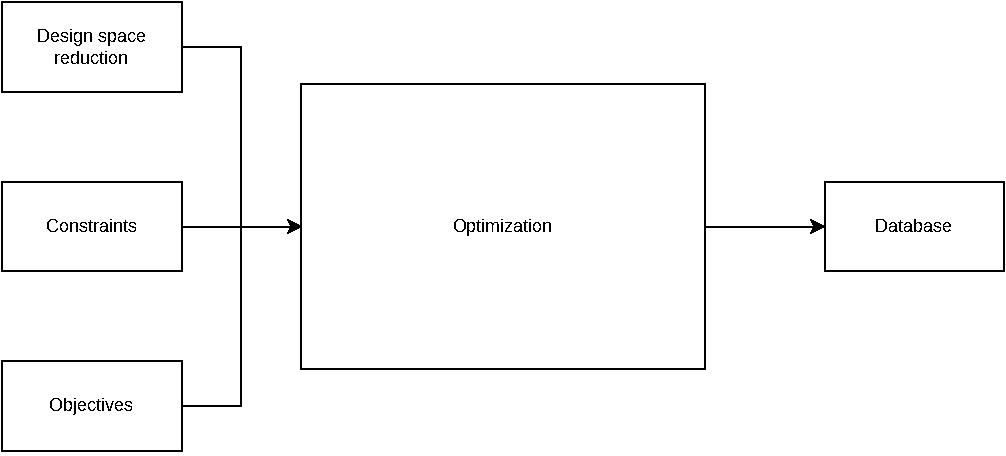
\includegraphics[page=1, scale=0.7]{pdf/databaseScheme-start.drawio}
        \end{figure}
    }
    \only<2>{
        \begin{figure}
            \centering
            \vspace*{0.5cm}
            \hspace*{0.3cm}
            \begin{tikzpicture}
    
    \node[draw,
        rectangle,
        text centered,
        line width = \PTS,
        minimum height = \TOTheight,
        minimum width = \TOTwidth
    ] (optimizationProcess) at (0, 0) {\large{\textbf{Optimization}}};

    % \node[
    %     below right = 0.5cm and 0.5cm of optimizationProcess.north west 
    % ] {
    %     
\includegraphics[scale=0.08]{./MITlogo.png}
    % };

    % \node[
    %     above left = 0.15cm and 0.5cm of optimizationProcess.south east 
    % ] {
    %     
\includegraphics[scale=0.3]{./SCIPYlogo.png}
    % };

    \node[draw,
        rectangle,
        text centered,
        line width = \PTS,
        % minimum width = \WIDTH,
        minimum height = \HEIGHT,
        right = 2*\xSpace of optimizationProcess
    ] (database) {\large{\textbf{Database}}};
    
    \coordinate[left=\xSpace of optimizationProcess.west]  (c1) {};
    \coordinate[above=\Ydist of c1]                      (c2) {};
    \coordinate[below=\Ydist of c1]                      (c3) {};

    \node[draw,
        rectangle,
        text centered,
        line width = \PTS,
        minimum width = \WIDTH,
        minimum height = \HEIGHT,
        left = \xSpace of c2
    ] (designSpace) {\large{\textbf{\makecell[c]{Kulfan\\parametrization}}}};

    \node[draw,
        rectangle,
        text centered,
        line width = \PTS,
        minimum width = \WIDTH,
        minimum height = \HEIGHT,
        left = \xSpace of c1
    ] (constr) {\large{\textbf{Constraints}}};

    \node[draw,
        rectangle,
        text centered,
        line width = \PTS,
        minimum width = \WIDTH,
        minimum height = \HEIGHT,
        left = \xSpace of c3
    ] (obj) {\large{\textbf{Objectives}}};

    \draw[-latex, line width = 1pt] (designSpace) -- (c2) -- (c1) to (optimizationProcess.west);
    \draw[-latex, line width = 1pt] (constr) to (optimizationProcess.west);
    \draw[-latex, line width = 1pt] (obj) -- (c3) -- (c1) to (optimizationProcess.west);
    \draw[-latex, line width = 1pt] (optimizationProcess.east) to (database.west);

\end{tikzpicture}
            % 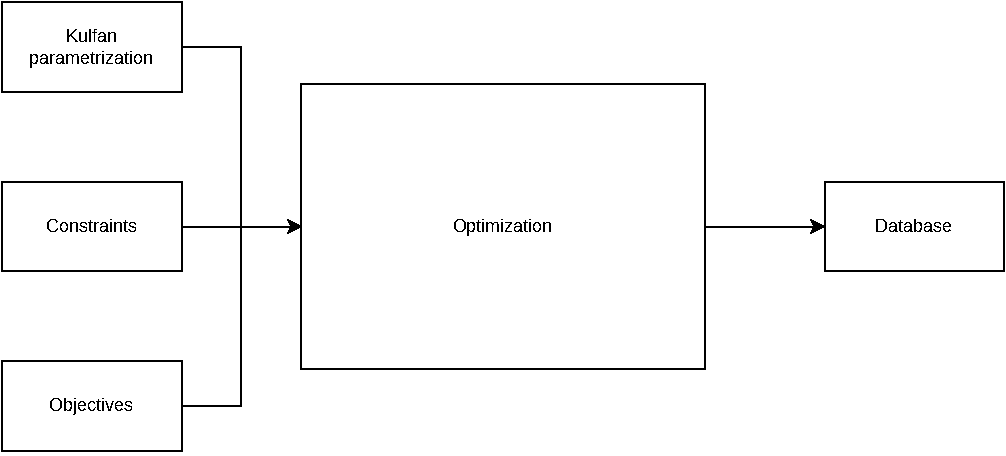
\includegraphics[page=1, scale=0.7]{pdf/databaseScheme-kulfan.drawio}
        \end{figure}
    }
    \only<3>{
        \begin{figure}
            \centering
            \vspace*{0.5cm}
            \hspace*{0.3cm}
            \begin{tikzpicture}
    
    \node[draw,
        rectangle,
        text centered,
        line width = \PTS,
        minimum height = \TOTheight,
        minimum width = \TOTwidth
    ] (optimizationProcess) at (0, 0) {\large{\textbf{Optimization}}};

    % \node[
    %     below right = 0.5cm and 0.5cm of optimizationProcess.north west 
    % ] {
    %     
\includegraphics[scale=0.08]{./MITlogo.png}
    % };

    % \node[
    %     above left = 0.15cm and 0.5cm of optimizationProcess.south east 
    % ] {
    %     
\includegraphics[scale=0.3]{./SCIPYlogo.png}
    % };

    \node[draw,
        rectangle,
        text centered,
        line width = \PTS,
        % minimum width = \WIDTH,
        minimum height = \HEIGHT,
        right = 2*\xSpace of optimizationProcess
    ] (database) {\large{\textbf{Database}}};
    
    \coordinate[left=\xSpace of optimizationProcess.west]  (c1) {};
    \coordinate[above=\Ydist of c1]                      (c2) {};
    \coordinate[below=\Ydist of c1]                      (c3) {};

    \node[draw,
        rectangle,
        text centered,
        line width = \PTS,
        minimum width = \WIDTH,
        minimum height = \HEIGHT,
        left = \xSpace of c2
    ] (designSpace) {\large{\textbf{\makecell[c]{Kulfan\\parametrization}}}};

    \node[draw,
        rectangle,
        text centered,
        line width = \PTS,
        minimum width = \WIDTH,
        minimum height = \HEIGHT,
        left = \xSpace of c1
    ] (constr) {\large{\textbf{\makecell[c]{Aerodynamic\\Duty}}}};

    \node[draw,
        rectangle,
        text centered,
        line width = \PTS,
        minimum width = \WIDTH,
        minimum height = \HEIGHT,
        left = \xSpace of c3
    ] (obj) {\large{\textbf{Objectives}}};

    \draw[-latex, line width = 1pt] (designSpace) -- (c2) -- (c1) to (optimizationProcess.west);
    \draw[-latex, line width = 1pt] (constr) to (optimizationProcess.west);
    \draw[-latex, line width = 1pt] (obj) -- (c3) -- (c1) to (optimizationProcess.west);
    \draw[-latex, line width = 1pt] (optimizationProcess.east) to (database.west);

\end{tikzpicture}
            % 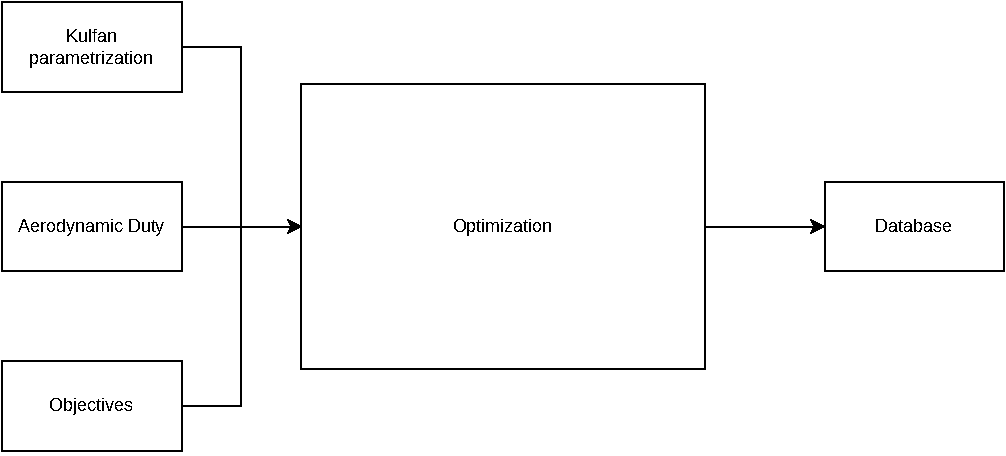
\includegraphics[page=1, scale=0.7]{pdf/databaseScheme-aerodynamicDuty.drawio}
        \end{figure}
    }
    \only<4>{
        \begin{figure}
            \centering
            \vspace*{0.5cm}
            \hspace*{0.3cm}
            \begin{tikzpicture}
    
    \node[draw,
        rectangle,
        text centered,
        line width = \PTS,
        minimum height = \TOTheight,
        minimum width = \TOTwidth
    ] (optimizationProcess) at (0, 0) {\large{\textbf{Optimization}}};

    % \node[
    %     below right = 0.5cm and 0.5cm of optimizationProcess.north west 
    % ] {
    %     
\includegraphics[scale=0.08]{./MITlogo.png}
    % };

    % \node[
    %     above left = 0.15cm and 0.5cm of optimizationProcess.south east 
    % ] {
    %     
\includegraphics[scale=0.3]{./SCIPYlogo.png}
    % };

    \node[draw,
        rectangle,
        text centered,
        line width = \PTS,
        % minimum width = \WIDTH,
        minimum height = \HEIGHT,
        right = 2*\xSpace of optimizationProcess
    ] (database) {\large{\textbf{Database}}};
    
    \coordinate[left=\xSpace of optimizationProcess.west]  (c1) {};
    \coordinate[above=\Ydist of c1]                      (c2) {};
    \coordinate[below=\Ydist of c1]                      (c3) {};

    \node[draw,
        rectangle,
        text centered,
        line width = \PTS,
        minimum width = \WIDTH,
        minimum height = \HEIGHT,
        left = \xSpace of c2
    ] (designSpace) {\large{\textbf{\makecell[c]{Kulfan\\parametrization}}}};

    \node[draw,
        rectangle,
        text centered,
        line width = \PTS,
        minimum width = \WIDTH,
        minimum height = \HEIGHT,
        left = \xSpace of c1
    ] (constr) {\large{\textbf{\makecell[c]{Aerodynamic\\Duty}}}};

    \node[draw,
        rectangle,
        text centered,
        line width = \PTS,
        minimum width = \WIDTH,
        minimum height = \HEIGHT,
        left = \xSpace of c3
    ] (obj) {\large{\textbf{\makecell[c]{Aerodynamic\\Style}}}};

    \draw[-latex, line width = 1pt] (designSpace) -- (c2) -- (c1) to (optimizationProcess.west);
    \draw[-latex, line width = 1pt] (constr) to (optimizationProcess.west);
    \draw[-latex, line width = 1pt] (obj) -- (c3) -- (c1) to (optimizationProcess.west);
    \draw[-latex, line width = 1pt] (optimizationProcess.east) to (database.west);

\end{tikzpicture}
            % 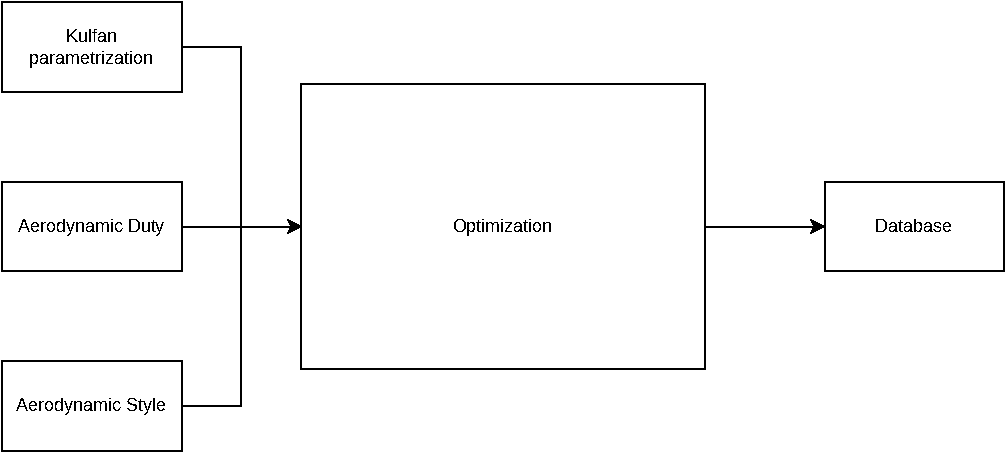
\includegraphics[page=1, scale=0.7]{pdf/databaseScheme-aerodynamicStyle.drawio}
        \end{figure}
    }
    \only<5>{
        \begin{figure}
            \centering
            \vspace*{0.5cm}
            \hspace*{0.3cm}
            \begin{tikzpicture}
    
    \node[draw,
        rectangle,
        text centered,
        line width = \PTS,
        minimum height = \TOTheight,
        minimum width = \TOTwidth
    ] (optimizationProcess) at (0, 0) {};

    \node[
        below right = 0.25cm and 0.25cm of optimizationProcess.north west 
    ] {
        
\includegraphics[scale=0.05]{./images/MITlogo.png}
    };

    \node[
        above left = 0.02cm and 0.02cm of optimizationProcess.south east 
    ] {
        
\includegraphics[scale=0.2]{./images/SCIPYlogo.png}
    };

    \node[draw,
        rectangle,
        text centered,
        line width = \PTS,
        % minimum width = 2cm,
        minimum height = \HEIGHT,
        right = 2*\xSpace of optimizationProcess
    ] (database) {\large{\textbf{Database}}};
    
    \coordinate[left=\xSpace of optimizationProcess.west]  (c1) {};
    \coordinate[above=\Ydist of c1]                      (c2) {};
    \coordinate[below=\Ydist of c1]                      (c3) {};

    \node[draw,
        rectangle,
        text centered,
        line width = \PTS,
        minimum width = \WIDTH,
        minimum height = \HEIGHT,
        left = \xSpace of c2
    ] (designSpace) {\large{\textbf{\makecell[c]{Kulfan\\parametrization}}}};

    \node[draw,
        rectangle,
        text centered,
        line width = \PTS,
        minimum width = \WIDTH,
        minimum height = \HEIGHT,
        left = \xSpace of c1
    ] (constr) {\large{\textbf{\makecell[c]{Aerodynamic\\Duty}}}};

    \node[draw,
        rectangle,
        text centered,
        line width = \PTS,
        minimum width = \WIDTH,
        minimum height = \HEIGHT,
        left = \xSpace of c3
    ] (obj) {\large{\textbf{\makecell[c]{Aerodynamic\\Style}}}};

    \draw[-latex, line width = 1pt] (designSpace) -- (c2) -- (c1) to (optimizationProcess.west);
    \draw[-latex, line width = 1pt] (constr) to (optimizationProcess.west);
    \draw[-latex, line width = 1pt] (obj) -- (c3) -- (c1) to (optimizationProcess.west);
    \draw[-latex, line width = 1pt] (optimizationProcess.east) to (database.west);

\end{tikzpicture}
            % 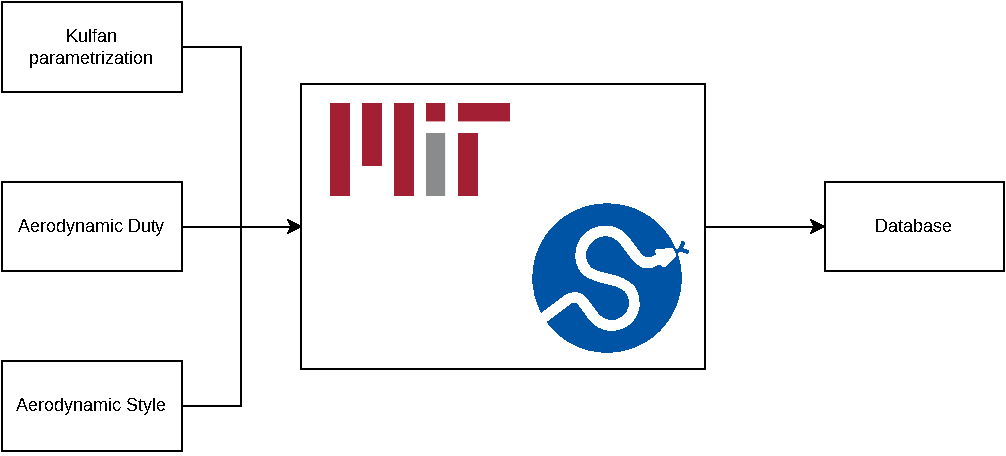
\includegraphics[page=1, scale=0.7]{pdf/databaseScheme-optimization.drawio}
        \end{figure}
    }
\end{frame}

\begin{frame}{Database points}
    \only<1>{
        \begin{columns}
            \column{0.5\textwidth}
            \begin{figure}
                \centering
                % \hspace*{-1cm}
                % \vspace{1cm}
                \includegraphics[scale=0.5]{images/staggerLinear.eps}
            \end{figure}
            \column{0.5\textwidth}
            \begin{itemize}
                \item Data optimization \textbf{starting from the boundaries of the domain} of study
                % \item From the \textbf{corner points} of the domain, it is \textbf{computed a new guess} for the optimization of the inner points
                % \item The new guess is made using a \textbf{linear interpolation} of optimized data 
                % \item Once this procedure generates \textbf{sufficient data for the ML training}, data collection is stopped
            \end{itemize}
        \end{columns}
    }
    \only<2>{
        \begin{columns}
            \column{0.5\textwidth}
            \begin{figure}
                \centering
                % \hspace*{-1cm}
                % \vspace{1cm}
                \includegraphics[scale=0.5]{images/staggerLinear1.eps}
            \end{figure}
            \column{0.5\textwidth}
            \begin{itemize}
                \item Data optimization \textbf{starting from the boundaries of the domain} of study
                \item From the \textbf{corner points} of the domain, it is \textbf{computed a new guess} for the optimization of the inner points
                \item The new guess is made using a \textbf{linear interpolation} of optimized data 
                % \item Once this procedure generates \textbf{sufficient data for the ML training}, data collection is stopped
            \end{itemize}
        \end{columns}
    }
    \only<3>{
        \begin{columns}
            \column{0.5\textwidth}
            \begin{figure}
                \centering
                % \hspace*{-1cm}
                % \vspace{1cm}
                \includegraphics[scale=0.5]{images/staggerLinear2.eps}
            \end{figure}
            \column{0.5\textwidth}
            \begin{itemize}
                \item Data optimization \textbf{starting from the boundaries of the domain} of study
                \item From the \textbf{corner points} of the domain, it is \textbf{computed a new guess} for the optimization of the inner points
                \item The new guess is made using a \textbf{linear interpolation} of optimized data 
                % \item Once this procedure generates \textbf{sufficient data for the ML training}, data collection is stopped
            \end{itemize}
        \end{columns}
    }
    \only<4>{
        \begin{columns}
            \column{0.5\textwidth}
            \begin{figure}
                \centering
                % \hspace*{-1cm}
                % \vspace{1cm}
                \includegraphics[scale=0.5]{images/staggerComplete.eps}
            \end{figure}
            \column{0.5\textwidth}
            \begin{itemize}
                \item Data optimization \textbf{starting from the boundaries of the domain} of study
                \item From the \textbf{corner points} of the domain, it is \textbf{computed a new guess} for the optimization of the inner points
                \item The new guess is made using a \textbf{linear interpolation} of optimized data 
                \item Once this procedure generates \textbf{sufficient data for the ML training}, data collection is stopped
            \end{itemize}
        \end{columns}
    }
\end{frame}

\begin{frame}{Inner points}
    The \textbf{new guess} on the blade shape for the inner points of the database is made by a \textbf{linear interpolation of the corner points} geometry.
    \begin{figure}
        \centering
        \includegraphics[page=1, scale=0.2]{./pdf/innerGeometry.pdf}
    \end{figure}
    From this guess, a \textbf{new optimization} of the inner point is made.
\end{frame}

\begin{frame}{Objectives \& constraints}
    \begin{columns}
        \column{0.5\textwidth}
            \begin{center}
                \renewcommand{\arraystretch}{2}
                \begin{tabularx}{1\textwidth} { 
                    || >{\centering\arraybackslash}X 
                    | >{\centering\arraybackslash}X 
                    | >{\centering\arraybackslash}X 
                    | >{\centering\arraybackslash}X || } 
                    \hline
                    Obj. & Min & Max & Points\\ [0.5ex] 
                    \hline\hline
                    $\frac{M_P}{M_{TE}}$ & $1.2$ & $1.4$ & 3 \\ [0.5ex]
                    \hline
                    $\frac{L_P}{L_{surf}}$ & $0.5$ & $0.6$ & 3 \\ [0.5ex]
                    \hline
                    $\frac{M_{LE}}{M_{TE}}\frac{M_2}{M_1}$ & $1.2$ & $1.8$ & 3 \\ [0.5ex]
                    \hline
                    $\frac{M_{PS}}{M_{TE}}\frac{M_2}{M_{1, ax}}$ & $0.8$ & $1.2$ & 3 \\ 
                    \hline
                \end{tabularx}
            \end{center}
        \column{0.5\textwidth}
            \begin{center}
                \renewcommand{\arraystretch}{2}
                \begin{tabularx}{1\textwidth} { 
                    || >{\centering\arraybackslash}X 
                    | >{\centering\arraybackslash}X 
                    | >{\centering\arraybackslash}X 
                    | >{\centering\arraybackslash}X || } 
                    \hline
                    Constr. & Min & Max & Points\\ [0.5ex] 
                    \hline\hline
                    $\alpha_1$ & $-50^{\circ}$ & $-20^{\circ}$ & 3 \\ [0.5ex]
                    \hline
                    $\alpha_2$ & $65^{\circ}$ & $72.5^{\circ}$ & 4 \\ [0.5ex]
                    \hline
                    $M_2$ & $0.4$ & $0.7$ & 3 \\ [0.5ex]
                    \hline
                    $Re$ & $6 \cdot 10^5$ & $6 \cdot 10^5$ & 1 \\ 
                    \hline
                \end{tabularx}
            \end{center}
    \end{columns}
\end{frame}

\subsection{Optimizer}
\SubSectionPage

\subsection{Optimization}

\begin{frame}
    \frametitle<1>{Nelder-Mead -- Simplex Method \Romannum{1}}
    \frametitle<2>{Nelder-Mead -- Simplex Method \Romannum{2}}
    \frametitle<3>{Nelder-Mead -- Simplex Method \Romannum{3}}
    \frametitle<4>{Nelder-Mead -- Simplex Method \Romannum{4}}
    \frametitle<5>{Nelder-Mead -- Simplex Method \Romannum{5}}
    \frametitle<6>{Nelder-Mead -- Simplex Method \Romannum{6}}
    
    \only<1>{
        \begin{columns}
            \column{0.5\textwidth}
                \begin{figure}[h!]
                    \begin{tikzpicture}[
    scale=0.24, 
    transform shape,
    thick,
    font = {\Huge\bfseries\sffamily},
    >=stealth',
    dot/.style = {
        draw,
        fill = white,
        circle,
        inner sep = 0pt,
        minimum size = 4pt
    }
    ]
  
    \coordinate (O) at (0,0);
    \draw[->] (-6,0) -- (12,0) coordinate[label = {below:$x$}] (xmax);
    \draw[->] (0,-5) -- (0,22) coordinate[label = {right:$y$}] (ymax);

    \node[
        color=red, 
        label = {below right:\color{red}{$X$}}
    ] (X) at (2.5, 2) {};

    \node[
        label = {below right:$c_0 = 10$}
    ] (P00) at (-2, -2) {};

    \node[ 
        label = {below right:$c_1 = 3$}
    ] (P10) at (10, 7) {};

    \node[
        label = {above right:$c_2 = 7$}
    ] (P20) at (1, 8) {};

    % DRAW TRIANGLE
    \fill[fill=gray!30, semitransparent] (P00.center)--(P10.center)--(P20.center);

    % DRAW LINES
    \draw[color=black, line width=1pt] (P00) -- (P10);
    \draw[color=black, line width=1pt] (P10) -- (P20);
    \draw[color=black, line width=1pt] (P20) -- (P00);

    % DRAW NODES
    \draw[color=black, line width=0.5pt] (P00) circle (.2);
    \draw[color=black, line width=0.5pt] (P10) circle (.2);
    \draw[color=black, line width=0.5pt] (P20) circle (.2);
    \draw[color=red, fill=white, line width=1pt, label={above right=$X$}] (X) circle (.25);

    % \node[
    %     color=black,
    %     line width=2pt,
    %     dot, 
    %     label = {above left:$c_0 = 12$}
    % ] (P01) at (2, 20) {};

    % % DRAW TRIANGLE
    % \fill[fill=green!30, semitransparent] (P01.center)--(P10.center)--(P20.center);
    
    % % DRAW NODES
    % \draw[color=black, line width=1.5pt] (P01) circle (.1);
    % \draw[color=black, line width=1.5pt] (P10) circle (.1);
    % \draw[color=black, line width=1.5pt] (P20) circle (.1);

    % % DRAW LINES
    % \draw[color=black, line width=1pt] (P01) -- (P10);
    % \draw[color=black, line width=1pt] (P10) -- (P20);
    % \draw[color=black, line width=1pt] (P20) -- (P01);

    % % DRAW LINES
    % \draw[color=black, line width=1pt] (P01) -- (P00);

    % \node[
    %     color=black,
    %     line width=2pt,
    %     dot, 
    %     label = {above left:$c_0 = 6$}
    % ] (P02) at (-1, 3.5) {};

    % % DRAW TRIANGLE
    % \fill[fill=red!30, semitransparent] (P02.center)--(P10.center)--(P20.center);

    % % DRAW NODES
    % \draw[color=black, line width=1.5pt] (P02) circle (.1);
    % \draw[color=black, line width=1.5pt] (P10) circle (.1);
    % \draw[color=black, line width=1.5pt] (P20) circle (.1);

    % % DRAW LINES
    % \draw[color=black, line width=1pt] (P02) -- (P10);
    % \draw[color=black, line width=1pt] (P10) -- (P20);
    % \draw[color=black, line width=1pt] (P20) -- (P02);

    % \node[
    %     color=black,
    %     line width=2pt,
    %     dot, 
    %     label = {below left:$c_0 = 0.2$}
    % ] (P21) at (2.1, 2) {};

    % % DRAW TRIANGLE
    % \fill[fill=yellow, pattern color=blue, semitransparent] (P02.center)--(P10.center)--(P21.center);

    % % DRAW NODES
    % \draw[color=black, line width=1.5pt] (P02) circle (.1);
    % \draw[color=black, line width=1.5pt] (P10) circle (.1);
    % \draw[color=black, line width=1.5pt] (P21) circle (.1);

    % % DRAW LINES
    % \draw[color=black, line width=1pt] (P02) -- (P10);
    % \draw[color=black, line width=1pt] (P10) -- (P21);
    % \draw[color=black, line width=1pt] (P21) -- (P02);

\end{tikzpicture}
                    % \begin{tikzpicture}[line cap=round,line join=round,>=triangle 45,x=1cm,y=1cm, scale=0.2]
\begin{axis}[
x=1cm,y=1cm,
axis lines=middle,
xmin=-11.683021640762064,
xmax=12.26720503650467,
ymin=-5.6693032180788805,
ymax=21.957373211560604,
xtick={-10,-8,...,10},
ytick={-4,-2,...,20},]
\clip(-11.683021640762064,-5.6693032180788805) rectangle (32.26720503650467,21.957373211560604);
\fill[line width=2pt,color=zzttqq,fill=zzttqq,fill opacity=0.19] (1.178695284830076,8.298938503258006) -- (-1.8923022147095834,-3.0058928718589892) -- (9.813094051651728,6.874707778833817) -- cycle;
\draw [line width=2pt,color=zzttqq] (1.178695284830076,8.298938503258006)-- (-1.8923022147095834,-3.0058928718589892);
\draw [line width=2pt,color=zzttqq] (-1.8923022147095834,-3.0058928718589892)-- (9.813094051651728,6.874707778833817);
\draw [line width=2pt,color=zzttqq] (9.813094051651728,6.874707778833817)-- (1.178695284830076,8.298938503258006);
\begin{scriptsize}
\draw [fill=ffqqqq] (3,2) circle (2.5pt);
\draw[color=ffqqqq] (3.234809868492963,2.6072244558058455) node {$X$};
\draw [fill=ududff] (1.178695284830076,8.298938503258006) circle (2.5pt);
\draw[color=ududff] (0.19386729160636174,8.516980784472237) node {cost = 1};
\draw [fill=ududff] (-1.8923022147095834,-3.0058928718589892) circle (2.5pt);
\draw[color=ududff] (-0.838905659034371,-3.3312200103783427) node {cost = 2};
\draw [fill=ududff] (9.813094051651728,6.874707778833817) circle (2.5pt);
\draw[color=ududff] (11.324864648512037,7.082573908582335) node {cost = 0.3};
\end{scriptsize}
\end{axis}
\end{tikzpicture}
                \end{figure}
            \column{0.55\textwidth}
                \begin{itemize}
                    \item The \color{red} X \color{black} point is the local minima.
                    \item The triangle points are the starting point of the optimization.
                    \item Each triangle point has a cost. 
                \end{itemize}
            \end{columns}
    }
    \only<2>{
        \begin{columns}
        \column{0.5\textwidth}
                \begin{figure}[h!]
                    \begin{tikzpicture}[
    scale=0.24, 
    transform shape,
    thick,
    font = {\Huge\bfseries\sffamily},
    >=stealth',
    dot/.style = {
        draw,
        fill = white,
        circle,
        inner sep = 0pt,
        minimum size = 4pt
    }
    ]
  
    \coordinate (O) at (0,0);
    \draw[->] (-6,0) -- (12,0) coordinate[label = {below:$x$}] (xmax);
    \draw[->] (0,-5) -- (0,22) coordinate[label = {right:$y$}] (ymax);

    \node[
        color=red, 
        label = {below right:\color{red}{$X$}}
    ] (X) at (2.5, 2) {};

    \node[
        label = {below right:$c_0 = 10$}
    ] (P00) at (-2, -2) {};

    \node[ 
        label = {below right:$c_1 = 3$}
    ] (P10) at (10, 7) {};

    \node[
        label = {above right:$c_2 = 7$}
    ] (P20) at (1, 8) {};

    % DRAW TRIANGLE
    \fill[semitransparent, pattern=north west lines, pattern color=gray] (P00.center)--(P10.center)--(P20.center);

    % DRAW LINES
    \draw[color=black, line width=1pt] (P00) -- (P10);
    \draw[color=black, line width=1pt] (P10) -- (P20);
    \draw[color=black, line width=1pt] (P20) -- (P00);

    \node[
        label = {above right:$c_0^{\prime} = 12$}
    ] (P01) at (2, 20) {};

    % DRAW TRIANGLE
    \fill[fill=green!30, semitransparent] (P01.center)--(P10.center)--(P20.center);
    
    % % DRAW NODES
    \draw[color=black, line width=0.5pt] (P01) circle (.2);
    % \draw[color=black, line width=1.5pt] (P10) circle (.1);
    % \draw[color=black, line width=1.5pt] (P20) circle (.1);

    % DRAW LINES
    \draw[color=black, line width=1pt] (P01) -- (P10);
    \draw[color=black, line width=1pt] (P10) -- (P20);
    \draw[color=black, line width=1pt] (P20) -- (P01);

    % DRAW NODES
    \draw[color=black, fill=white, line width=0.5pt] (P00) circle (.2);
    \draw[color=black, fill=white, line width=0.5pt] (P10) circle (.2);
    \draw[color=black, fill=white, line width=0.5pt] (P20) circle (.2);
    \draw[color=red, fill=white, line width=1pt, label={above right=$X$}] (X) circle (.25);

    \node[
        label = {above right:$c_2 = 7$}
    ] (P20c) at (1, 8) {};

    \draw[color=black, fill=white, line width=0.5pt] (P20c) circle (.2);

    % % DRAW LINES
    % \draw[color=black, line width=1pt] (P01) -- (P00);

    % \node[
    %     color=black,
    %     line width=2pt,
    %     dot, 
    %     label = {above left:$c_0 = 6$}
    % ] (P02) at (-1, 3.5) {};

    % % DRAW TRIANGLE
    % \fill[fill=red!30, semitransparent] (P02.center)--(P10.center)--(P20.center);

    % % DRAW NODES
    % \draw[color=black, line width=1.5pt] (P02) circle (.1);
    % \draw[color=black, line width=1.5pt] (P10) circle (.1);
    % \draw[color=black, line width=1.5pt] (P20) circle (.1);

    % % DRAW LINES
    % \draw[color=black, line width=1pt] (P02) -- (P10);
    % \draw[color=black, line width=1pt] (P10) -- (P20);
    % \draw[color=black, line width=1pt] (P20) -- (P02);

    % \node[
    %     color=black,
    %     line width=2pt,
    %     dot, 
    %     label = {below left:$c_0 = 0.2$}
    % ] (P21) at (2.1, 2) {};

    % % DRAW TRIANGLE
    % \fill[fill=yellow, pattern color=blue, semitransparent] (P02.center)--(P10.center)--(P21.center);

    % % DRAW NODES
    % \draw[color=black, line width=1.5pt] (P02) circle (.1);
    % \draw[color=black, line width=1.5pt] (P10) circle (.1);
    % \draw[color=black, line width=1.5pt] (P21) circle (.1);

    % % DRAW LINES
    % \draw[color=black, line width=1pt] (P02) -- (P10);
    % \draw[color=black, line width=1pt] (P10) -- (P21);
    % \draw[color=black, line width=1pt] (P21) -- (P02);

\end{tikzpicture}
                    % \begin{tikzpicture}[line cap=round,line join=round,>=triangle 45,x=1cm,y=1cm, scale=0.2]
\begin{axis}[
x=1cm,y=1cm,
axis lines=middle,
xmin=-11.683021640762064,
xmax=12.26720503650467,
ymin=-5.6693032180788805,
ymax=21.957373211560604,
xtick={-10,-8,...,10},
ytick={-4,-2,...,20},]
\clip(-11.683021640762064,-5.6693032180788805) rectangle (32.26720503650467,21.957373211560604);
\fill[line width=2.4pt,color=zzttqq,fill=zzttqq,pattern=dots,pattern color=zzttqq] (1.178695284830076,8.298938503258006) -- (-1.8923022147095834,-3.0058928718589892) -- (9.813094051651728,6.874707778833817) -- cycle;
\fill[line width=2pt,color=qqzzqq,fill=qqzzqq,fill opacity=0.46] (1.178695284830076,8.298938503258006) -- (9.813094051651728,6.874707778833817) -- (1.9010291156709027,19.991178318572743) -- cycle;
\draw [line width=2.4pt,color=zzttqq] (1.178695284830076,8.298938503258006)-- (-1.8923022147095834,-3.0058928718589892);
\draw [line width=2.4pt,color=zzttqq] (-1.8923022147095834,-3.0058928718589892)-- (9.813094051651728,6.874707778833817);
\draw [line width=2.4pt,color=zzttqq] (9.813094051651728,6.874707778833817)-- (1.178695284830076,8.298938503258006);
\draw [line width=2pt,color=qqzzqq] (1.178695284830076,8.298938503258006)-- (9.813094051651728,6.874707778833817);
\draw [line width=2pt,color=qqzzqq] (9.813094051651728,6.874707778833817)-- (1.9010291156709027,19.991178318572743);
\draw [line width=2pt,color=qqzzqq] (1.9010291156709027,19.991178318572743)-- (1.178695284830076,8.298938503258006);
\begin{scriptsize}
\draw [fill=ffqqqq] (3,2) circle (2.5pt);
\draw[color=ffqqqq] (3.234809868492963,2.6072244558058455) node {$X$};
\draw [fill=ududff] (1.178695284830076,8.298938503258006) circle (2.5pt);
\draw[color=ududff] (0.19386729160636174,8.516980784472237) node {cost = 1};
\draw [fill=ududff] (-1.8923022147095834,-3.0058928718589892) circle (2.5pt);
\draw[color=ududff] (-0.838905659034371,-3.3312200103783427) node {cost = 2};
\draw [fill=ududff] (9.813094051651728,6.874707778833817) circle (2.5pt);
\draw[color=ududff] (11.324864648512037,7.082573908582335) node {cost = 0.3};
\draw [fill=ududff] (1.9010291156709027,19.991178318572743) circle (2.5pt);
\draw[color=ududff] (2.947928493314982,20.594686679465198) node {cost = 4};
\end{scriptsize}
\end{axis}
\end{tikzpicture}
                \end{figure} 
            \column{0.55\textwidth}
            \begin{itemize}
                \item The \color{red} X \color{black} point is the local minima.
                {\transparent{0.4}
                \item The triangle points are the starting point of the optimization.
                \item Each triangle point has a cost. 
                }
                \item A new point is computed mirroring the point with highest cost.
                \item The cost of the new point is computed.
            \end{itemize}
        \end{columns}
    \begin{figure}
    \end{figure}
    }
    \only<3>{
        \begin{columns}
        \column{0.5\textwidth}
                \begin{figure}[h!]
                    \begin{tikzpicture}[
    scale=0.24, 
    transform shape,
    thick,
    font = {\Huge\bfseries\sffamily},
    >=stealth',
    dot/.style = {
        draw,
        fill = white,
        circle,
        inner sep = 0pt,
        minimum size = 4pt
    }
    ]
  
    \coordinate (O) at (0,0);
    \draw[->] (-6,0) -- (12,0) coordinate[label = {below:$x$}] (xmax);
    \draw[->] (0,-5) -- (0,22) coordinate[label = {right:$y$}] (ymax);

    \node[
        color=red, 
        label = {below right:\color{red}{$X$}}
    ] (X) at (2.5, 2) {};

    \node[
        label = {below right:$c_0 = 10$}
    ] (P00) at (-2, -2) {};

    \node[ 
        label = {below right:$c_1 = 3$}
    ] (P10) at (10, 7) {};

    \node[
        label = {above right:$c_2 = 7$}
    ] (P20) at (1, 8) {};

    % DRAW TRIANGLE
    \fill[semitransparent, pattern=north west lines, pattern color=gray] (P00.center)--(P10.center)--(P20.center);

    % DRAW LINES
    \draw[color=black, line width=1pt] (P00) -- (P10);
    \draw[color=black, line width=1pt] (P10) -- (P20);
    \draw[color=black, line width=1pt] (P20) -- (P00);

    \node[
        label = {above right:$c_0^{\prime} = 12$}
    ] (P01) at (2, 20) {};

    % DRAW TRIANGLE
    \fill[semitransparent, pattern=north west lines, pattern color=green] (P01.center)--(P10.center)--(P20.center);
    
    % % DRAW NODES
    \draw[color=black, line width=0.5pt] (P01) circle (.2);

    % DRAW NODES
    \draw[color=black, fill=white, line width=0.5pt] (P00) circle (.2);
    \draw[color=black, fill=white, line width=0.5pt] (P10) circle (.2);
    \draw[color=black, fill=white, line width=0.5pt] (P20) circle (.2);
    \draw[color=red, fill=white, line width=1pt, label={above right=$X$}] (X) circle (.25);

    \node[
        label = {above right:$c_2 = 7$}
    ] (P20c) at (1, 8) {};

    \draw[color=black, fill=white, line width=0.5pt] (P20c) circle (.2);

    % \draw[color=black, line width=1.5pt] (P10) circle (.1);
    % \draw[color=black, line width=1.5pt] (P20) circle (.1);

    % DRAW LINES
    \draw[color=black, line width=1pt] (P01) -- (P10);
    \draw[color=black, line width=1pt] (P10) -- (P20);
    \draw[color=black, line width=1pt] (P20) -- (P01);

    % DRAW LINES
    \draw[color=black, line width=1pt] (P01) -- (P00);

    \node[
        label = {above left:$c_0^{\prime \prime} = 6$}
    ] (P02) at (-1, 3.5) {};

    % DRAW TRIANGLE
    % \fill[fill=red!30, semitransparent] (P02.center)--(P10.center)--(P20.center);

    % DRAW NODES
    \draw[color=black, fill=white, line width=0.5pt] (P02) circle (.2);
    % \draw[color=black, line width=1.5pt] (P10) circle (.1);
    % \draw[color=black, line width=1.5pt] (P20) circle (.1);

    % % DRAW LINES
    % \draw[color=black, line width=1pt] (P02) -- (P10);
    % \draw[color=black, line width=1pt] (P10) -- (P20);
    % \draw[color=black, line width=1pt] (P20) -- (P02);

    % \node[
    %     color=black,
    %     line width=2pt,
    %     dot, 
    %     label = {below left:$c_0 = 0.2$}
    % ] (P21) at (2.1, 2) {};

    % % DRAW TRIANGLE
    % \fill[fill=yellow, pattern color=blue, semitransparent] (P02.center)--(P10.center)--(P21.center);

    % % DRAW NODES
    % \draw[color=black, line width=1.5pt] (P02) circle (.1);
    % \draw[color=black, line width=1.5pt] (P10) circle (.1);
    % \draw[color=black, line width=1.5pt] (P21) circle (.1);

    % % DRAW LINES
    % \draw[color=black, line width=1pt] (P02) -- (P10);
    % \draw[color=black, line width=1pt] (P10) -- (P21);
    % \draw[color=black, line width=1pt] (P21) -- (P02);

\end{tikzpicture}
                    % \begin{tikzpicture}[line cap=round,line join=round,>=triangle 45,x=1cm,y=1cm, scale=0.2]
\begin{axis}[
x=1cm,y=1cm,
axis lines=middle,
xmin=-11.683021640762064,
xmax=12.267205036504684,
ymin=-5.6693032180788805,
ymax=21.957373211560604,
xtick={-10,-8,...,10},
ytick={-4,-2,...,20},]
\clip(-11.683021640762064,-5.6693032180788805) rectangle (32.267205036504684,21.957373211560604);
\fill[line width=2.4pt,color=zzttqq,fill=zzttqq,pattern=dots,pattern color=zzttqq] (1.178695284830076,8.298938503258006) -- (-1.8923022147095834,-3.0058928718589892) -- (9.813094051651728,6.874707778833817) -- cycle;
\fill[line width=2pt,color=qqzzqq,fill=qqzzqq,pattern=dots,pattern color=qqzzqq] (1.178695284830076,8.298938503258006) -- (9.813094051651728,6.874707778833817) -- (1.9010291156709027,19.991178318572743) -- cycle;
\draw [line width=2.4pt,color=zzttqq] (1.178695284830076,8.298938503258006)-- (-1.8923022147095834,-3.0058928718589892);
\draw [line width=2.4pt,color=zzttqq] (-1.8923022147095834,-3.0058928718589892)-- (9.813094051651728,6.874707778833817);
\draw [line width=2.4pt,color=zzttqq] (9.813094051651728,6.874707778833817)-- (1.178695284830076,8.298938503258006);
\draw [line width=2pt,color=qqzzqq] (1.178695284830076,8.298938503258006)-- (9.813094051651728,6.874707778833817);
\draw [line width=2pt,color=qqzzqq] (9.813094051651728,6.874707778833817)-- (1.9010291156709027,19.991178318572743);
\draw [line width=2pt,color=qqzzqq] (1.9010291156709027,19.991178318572743)-- (1.178695284830076,8.298938503258006);
\draw [line width=2pt,domain=-11.683021640762064:32.267205036504684] plot(\x,{(-32.115061138897836-22.997071190431733*\x)/-3.793331330380486});
\begin{scriptsize}
\draw [fill=ffqqqq] (3,2) circle (2.5pt);
\draw[color=ffqqqq] (3.234809868492967,2.6072244558058455) node {$X$};
\draw [fill=ududff] (1.178695284830076,8.298938503258006) circle (2.5pt);
\draw[color=ududff] (0.19386729160636496,8.516980784472237) node {cost = 1};
\draw [fill=ududff] (-1.8923022147095834,-3.0058928718589892) circle (2.5pt);
\draw[color=ududff] (-0.8389056590343679,-3.3312200103783427) node {cost = 2};
\draw [fill=ududff] (9.813094051651728,6.874707778833817) circle (2.5pt);
\draw[color=ududff] (11.324864648512042,7.082573908582335) node {cost = 0.3};
\draw [fill=ududff] (1.9010291156709027,19.991178318572743) circle (2.5pt);
\draw[color=ududff] (2.9479284933149863,20.594686679465198) node {cost = 4};
\draw [fill=xdxdff] (-0.6433892210348795,4.565642152293915) circle (2.5pt);
\draw[color=xdxdff] (-1.6708616470505138,5.361285657514454) node {cost = 0.2};
\end{scriptsize}
\end{axis}
\end{tikzpicture}
                \end{figure} 
            \column{0.55\textwidth}
            \begin{itemize}
                \item The \color{red} X \color{black} point is the local minima.
                {\transparent{0.4}
                \item The triangle points are the starting point of the optimization.
                \item Each triangle point has a cost. 
                \item A new point is computed mirroring the point with highest cost.
                \item The cost of the new point is computed.
                } 
                \item If the cost of the new point is greater than its parent, a new point is found over their conjunction line.
                \item The cost of the new point is computed.
            \end{itemize}
         \end{columns}
    }
    \only<4>{
        \begin{columns}
            \column{0.5\textwidth}
                    \begin{figure}[h!]
                        \begin{tikzpicture}[
    scale=0.24, 
    transform shape,
    thick,
    font = {\Huge\bfseries\sffamily},
    >=stealth',
    dot/.style = {
        draw,
        fill = white,
        circle,
        inner sep = 0pt,
        minimum size = 4pt
    }
    ]
  
    \coordinate (O) at (0,0);
    \draw[->] (-6,0) -- (12,0) coordinate[label = {below:$x$}] (xmax);
    \draw[->] (0,-5) -- (0,22) coordinate[label = {right:$y$}] (ymax);

    \node[
        color=red, 
        label = {below right:\color{red}{$X$}}
    ] (X) at (2.5, 2) {};

    % \node[
    %     label = {below right:$c_0 = 10$}
    % ] (P00) at (-2, -2) {};

    \node[ 
        label = {below right:$c_1 = 3$}
    ] (P10) at (10, 7) {};

    \node[
        label = {above right:$c_2 = 7$}
    ] (P20) at (1, 8) {};

    % DRAW TRIANGLE
    % \fill[semitransparent, pattern=north west lines, pattern color=gray] (P00.center)--(P10.center)--(P20.center);

    % DRAW LINES
    % \draw[color=black, line width=1pt] (P00) -- (P10);
    % \draw[color=black, line width=1pt] (P10) -- (P20);
    % \draw[color=black, line width=1pt] (P20) -- (P00);

    % DRAW NODES
    % \draw[color=black, fill=white, line width=0.5pt] (P00) circle (.2);
    \draw[color=black, fill=white, line width=0.5pt] (P10) circle (.2);
    \draw[color=black, fill=white, line width=0.5pt] (P20) circle (.2);
    \draw[color=red, fill=white, line width=1pt, label={above right=$X$}] (X) circle (.25);

    % \node[
    %     label = {above right:$c_0 = 12$}
    % ] (P01) at (2, 20) {};

    % DRAW TRIANGLE
    % \fill[semitransparent, pattern=north west lines, pattern color=green] (P01.center)--(P10.center)--(P20.center);
    
    % % DRAW NODES
    % \draw[color=black, line width=0.5pt] (P01) circle (.2);
    % \draw[color=black, line width=1.5pt] (P10) circle (.1);
    % \draw[color=black, line width=1.5pt] (P20) circle (.1);

    % DRAW LINES
    % \draw[color=black, line width=1pt] (P01) -- (P10);
    % \draw[color=black, line width=1pt] (P10) -- (P20);
    % \draw[color=black, line width=1pt] (P20) -- (P01);

    % DRAW LINES
    % \draw[color=black, line width=1pt] (P01) -- (P00);

    \node[
        label = {above left:$c_0 = 6$}
    ] (P02) at (-1, 3.5) {};

    % DRAW TRIANGLE
    \fill[fill=red!30, semitransparent] (P02.center)--(P10.center)--(P20.center);

    % DRAW NODES
    \draw[color=black, fill=white, line width=0.5pt] (P02) circle (.2);
    \draw[color=black, fill=white, line width=0.5pt] (P10) circle (.2);
    \draw[color=black, fill=white, line width=0.5pt] (P20) circle (.2);

    % % DRAW LINES
    \draw[color=black, line width=1pt] (P02) -- (P10);
    \draw[color=black, line width=1pt] (P10) -- (P20);
    \draw[color=black, line width=1pt] (P20) -- (P02);

    % \node[
    %     color=black,
    %     line width=2pt,
    %     dot, 
    %     label = {below left:$c_0 = 0.2$}
    % ] (P21) at (2.1, 2) {};

    % % DRAW TRIANGLE
    % \fill[fill=yellow, pattern color=blue, semitransparent] (P02.center)--(P10.center)--(P21.center);

    % % DRAW NODES
    % \draw[color=black, line width=1.5pt] (P02) circle (.1);
    % \draw[color=black, line width=1.5pt] (P10) circle (.1);
    % \draw[color=black, line width=1.5pt] (P21) circle (.1);

    % % DRAW LINES
    % \draw[color=black, line width=1pt] (P02) -- (P10);
    % \draw[color=black, line width=1pt] (P10) -- (P21);
    % \draw[color=black, line width=1pt] (P21) -- (P02);

\end{tikzpicture}
                        % \begin{tikzpicture}[line cap=round,line join=round,>=triangle 45,x=1cm,y=1cm, scale=0.2]
\begin{axis}[
x=1cm,y=1cm,
axis lines=middle,
xmin=-11.683021640762064,
xmax=12.267205036504684,
ymin=-5.6693032180788805,
ymax=21.957373211560604,
xtick={-10,-8,...,10},
ytick={-4,-2,...,20},]
\clip(-11.683021640762064,-5.6693032180788805) rectangle (32.267205036504684,21.957373211560604);
\fill[line width=2pt,color=ffqqqq,fill=ffqqqq,fill opacity=0.1] (1.178695284830076,8.298938503258006) -- (9.813094051651728,6.874707778833817) -- (-0.6433892210348795,4.565642152293915) -- cycle;
\draw [line width=2pt,color=ffqqqq] (1.178695284830076,8.298938503258006)-- (9.813094051651728,6.874707778833817);
\draw [line width=2pt,color=ffqqqq] (9.813094051651728,6.874707778833817)-- (-0.6433892210348795,4.565642152293915);
\draw [line width=2pt,color=ffqqqq] (-0.6433892210348795,4.565642152293915)-- (1.178695284830076,8.298938503258006);
\begin{scriptsize}
\draw [fill=ffqqqq] (3,2) circle (2.5pt);
\draw[color=ffqqqq] (3.234809868492967,2.6072244558058455) node {$X$};
\draw [fill=ududff] (1.178695284830076,8.298938503258006) circle (2.5pt);
\draw[color=ududff] (0.19386729160636496,8.516980784472237) node {cost = 1};
\draw [fill=ududff] (9.813094051651728,6.874707778833817) circle (2.5pt);
\draw[color=ududff] (11.324864648512042,7.082573908582335) node {cost = 0.3};
\draw [fill=xdxdff] (-0.6433892210348795,4.565642152293915) circle (2.5pt);
\draw[color=xdxdff] (-1.6708616470505138,5.361285657514454) node {cost = 0.2};
\end{scriptsize}
\end{axis}
\end{tikzpicture}
                    \end{figure} 
            \column{0.55\textwidth}
            \begin{itemize}
                \item The \color{red} X \color{black} point is the local minima.
                {\transparent{0.4}
                \item The triangle points are the starting point of the optimization.
                \item Each triangle point has a cost. 
                \item A new point is computed mirroring the point with highest cost.
                \item The cost of the new point is computed.
                \item If the cost of the new point is greater than its parent, a new point is found over their conjunction line.
                \item The cost of the new point is computed.
                }
                \item A new study triangle is generated for the next optimization step. 
            \end{itemize}
        \end{columns}
    }
    \only<5>{
        % \vspace{-1.2cm} 
        \begin{columns}
            \column{0.5\textwidth}
                \begin{figure}[h!]
                    \begin{tikzpicture}[
    scale=0.24, 
    transform shape,
    thick,
    font = {\Huge\bfseries\sffamily},
    >=stealth',
    dot/.style = {
        draw,
        fill = white,
        circle,
        inner sep = 0pt,
        minimum size = 4pt
    }
    ]
  
    \coordinate (O) at (0,0);
    \draw[->] (-6,0) -- (12,0) coordinate[label = {below:$x$}] (xmax);
    \draw[->] (0,-5) -- (0,22) coordinate[label = {right:$y$}] (ymax);

    \node[
        color=red, 
        label = {below right:\color{red}{$X$}}
    ] (X) at (2.5, 2) {};

    % \node[
    %     label = {below right:$c_0 = 10$}
    % ] (P00) at (-2, -2) {};

    \node[ 
        label = {below right:$c_1 = 3$}
    ] (P10) at (10, 7) {};

    \node[
        label = {above right:$c_2 = 7$}
    ] (P20) at (1, 8) {};

    % DRAW TRIANGLE
    % \fill[semitransparent, pattern=north west lines, pattern color=gray] (P00.center)--(P10.center)--(P20.center);

    % DRAW LINES
    % \draw[color=black, line width=1pt] (P00) -- (P10);
    % \draw[color=black, line width=1pt] (P10) -- (P20);
    % \draw[color=black, line width=1pt] (P20) -- (P00);

    % DRAW NODES
    % \draw[color=black, fill=white, line width=0.5pt] (P00) circle (.2);
    \draw[color=black, fill=white, line width=0.5pt] (P10) circle (.2);
    \draw[color=black, fill=white, line width=0.5pt] (P20) circle (.2);
    \draw[color=red, fill=white, line width=1pt, label={below right=$X$}] (X) circle (.25);

    % \node[
    %     label = {above right:$c_0 = 12$}
    % ] (P01) at (2, 20) {};

    % DRAW TRIANGLE
    % \fill[semitransparent, pattern=north west lines, pattern color=green] (P01.center)--(P10.center)--(P20.center);
    
    % % DRAW NODES
    % \draw[color=black, line width=0.5pt] (P01) circle (.2);
    % \draw[color=black, line width=1.5pt] (P10) circle (.1);
    % \draw[color=black, line width=1.5pt] (P20) circle (.1);

    % DRAW LINES
    % \draw[color=black, line width=1pt] (P01) -- (P10);
    % \draw[color=black, line width=1pt] (P10) -- (P20);
    % \draw[color=black, line width=1pt] (P20) -- (P01);

    % DRAW LINES
    % \draw[color=black, line width=1pt] (P01) -- (P00);

    \node[
        label = {above left:$c_0 = 6$}
    ] (P02) at (-1, 3.5) {};

    % DRAW TRIANGLE
    \fill[semitransparent, pattern=north west lines, pattern color=red] (P02.center)--(P10.center)--(P20.center);

    % DRAW NODES
    \draw[color=black, fill=white, line width=0.5pt] (P02) circle (.2);
    \draw[color=black, fill=white, line width=0.5pt] (P10) circle (.2);
    \draw[color=black, fill=white, line width=0.5pt] (P20) circle (.2);

    % % DRAW LINES
    \draw[color=black, line width=1pt] (P02) -- (P10);
    \draw[color=black, line width=1pt] (P10) -- (P20);
    \draw[color=black, line width=1pt] (P20) -- (P02);

    \node[
        label = {below left:$c_2^{\prime} = 0.2$}
    ] (P21) at (2.1, 2) {};

    % DRAW TRIANGLE
    \fill[fill=yellow, pattern color=blue, semitransparent] (P02.center)--(P10.center)--(P21.center);

    % DRAW NODES
    \draw[color=black, fill=white, line width=0.5pt] (P02) circle (.2);
    \draw[color=black, fill=white, line width=0.5pt] (P10) circle (.2);
    \draw[color=black, fill=white, line width=0.5pt] (P21) circle (.2);

    % DRAW LINES
    \draw[color=black, line width=1pt] (P02) -- (P10);
    \draw[color=black, line width=1pt] (P10) -- (P21);
    \draw[color=black, line width=1pt] (P21) -- (P02);

\end{tikzpicture}
                    % \begin{tikzpicture}[line cap=round,line join=round,>=triangle 45,x=1cm,y=1cm, scale=0.2]
\begin{axis}[
x=1cm,y=1cm,
axis lines=middle,
xmin=-11.683021640762064,
xmax=12.267205036504684,
ymin=-5.6693032180788805,
ymax=21.957373211560604,
xtick={-10,-8,...,10},
ytick={-4,-2,...,20},]
\clip(-11.683021640762064,-5.6693032180788805) rectangle (32.267205036504684,21.957373211560604);
\fill[line width=2pt,color=ffqqqq,fill=ffqqqq,pattern=dots,pattern color=ffqqqq] (-0.6433892210348795,4.565642152293915) -- (9.813094051651728,6.874707778833817) -- (1.178695284830076,8.298938503258006) -- cycle;
\fill[line width=2pt,color=ffzzqq,fill=ffzzqq,fill opacity=0.1] (-0.6433892210348795,4.565642152293915) -- (2.5814074802324525,1.9468294774104518) -- (9.813094051651728,6.874707778833817) -- cycle;
\draw [line width=2pt,color=ffqqqq] (-0.6433892210348795,4.565642152293915)-- (9.813094051651728,6.874707778833817);
\draw [line width=2pt,color=ffqqqq] (9.813094051651728,6.874707778833817)-- (1.178695284830076,8.298938503258006);
\draw [line width=2pt,color=ffqqqq] (1.178695284830076,8.298938503258006)-- (-0.6433892210348795,4.565642152293915);
\draw [line width=2pt,color=ffzzqq] (-0.6433892210348795,4.565642152293915)-- (2.5814074802324525,1.9468294774104518);
\draw [line width=2pt,color=ffzzqq] (2.5814074802324525,1.9468294774104518)-- (9.813094051651728,6.874707778833817);
\draw [line width=2pt,color=ffzzqq] (9.813094051651728,6.874707778833817)-- (-0.6433892210348795,4.565642152293915);
\begin{scriptsize}
\draw [fill=ffqqqq] (3,2) circle (2.5pt);
\draw[color=ffqqqq] (3.234809868492967,2.6072244558058455) node {$X$};
\draw [fill=ududff] (1.178695284830076,8.298938503258006) circle (2.5pt);
\draw[color=ududff] (0.19386729160636496,8.516980784472237) node {cost = 1};
\draw [fill=ududff] (9.813094051651728,6.874707778833817) circle (2.5pt);
\draw[color=ududff] (11.324864648512042,7.082573908582335) node {cost = 0.3};
\draw [fill=xdxdff] (-0.6433892210348795,4.565642152293915) circle (2.5pt);
\draw[color=xdxdff] (-1.6708616470505138,5.361285657514454) node {cost = 0.2};
\draw [fill=ududff] (2.5814074802324525,1.9468294774104518) circle (2.5pt);
\draw[color=ududff] (1.685650442531868,2.8367295559482297) node {cost = 0.01};
\end{scriptsize}
\end{axis}
\end{tikzpicture}
                \end{figure} 
            \column{0.55\textwidth}
            \begin{itemize}
                \item The \color{red} X \color{black} point is the local minima.
                {\transparent{0.4}
                \item ...
                \item The cost of the new point is computed.
                \item If the cost of the new point is greater than its parent, a new point is found over their conjunction line.
                \item The cost of the new point is computed.
                \item A new study triangle is generated for the next optimization step. 
                }
                \item The algorithm is repeated till convergence is reached.        
            \end{itemize}
        \end{columns}
    }
    \only<6>{
        \begin{columns}
            \column{0.5\textwidth}
                    \begin{figure}[h!]
                        \begin{tikzpicture}[
    scale=0.24, 
    transform shape,
    thick,
    font = {\Huge\bfseries\sffamily},
    >=stealth',
    dot/.style = {
        draw,
        fill = white,
        circle,
        inner sep = 0pt,
        minimum size = 4pt
    }
    ]
  
    \coordinate (O) at (0,0);
    \draw[->] (-6,0) -- (12,0) coordinate[label = {below:$x$}] (xmax);
    \draw[->] (0,-5) -- (0,22) coordinate[label = {right:$y$}] (ymax);

    \node[
        color=red, 
        label = {below right:\color{red}{$X$}}
    ] (X) at (2.5, 2) {};

    % \node[
    %     label = {below right:$c_0 = 10$}
    % ] (P00) at (-2, -2) {};

    \node[ 
        label = {below right:$c_1 = 3$}
    ] (P10) at (10, 7) {};

    % \node[
    %     label = {above right:$c_2 = 1$}
    % ] (P20) at (1, 8) {};

    % DRAW TRIANGLE
    % \fill[semitransparent, pattern=north west lines, pattern color=gray] (P00.center)--(P10.center)--(P20.center);

    % DRAW LINES
    % \draw[color=black, line width=1pt] (P00) -- (P10);
    % \draw[color=black, line width=1pt] (P10) -- (P20);
    % \draw[color=black, line width=1pt] (P20) -- (P00);

    % DRAW NODES
    % \draw[color=black, fill=white, line width=0.5pt] (P00) circle (.2);
    \draw[color=black, fill=white, line width=0.5pt] (P10) circle (.2);
    % \draw[color=black, fill=white, line width=0.5pt] (P20) circle (.2);
    \draw[color=red, fill=white, line width=1pt, label={below right=$X$}] (X) circle (.25);

    % \node[
    %     label = {above right:$c_0 = 12$}
    % ] (P01) at (2, 20) {};

    % DRAW TRIANGLE
    % \fill[semitransparent, pattern=north west lines, pattern color=green] (P01.center)--(P10.center)--(P20.center);
    
    % % DRAW NODES
    % \draw[color=black, line width=0.5pt] (P01) circle (.2);
    % \draw[color=black, line width=1.5pt] (P10) circle (.1);
    % \draw[color=black, line width=1.5pt] (P20) circle (.1);

    % DRAW LINES
    % \draw[color=black, line width=1pt] (P01) -- (P10);
    % \draw[color=black, line width=1pt] (P10) -- (P20);
    % \draw[color=black, line width=1pt] (P20) -- (P01);

    % DRAW LINES
    % \draw[color=black, line width=1pt] (P01) -- (P00);

    \node[
        label = {above left:$c_0 = 6$}
    ] (P02) at (-1, 3.5) {};

    % % DRAW TRIANGLE
    % \fill[semitransparent, pattern=north west lines, pattern color=red] (P02.center)--(P10.center)--(P20.center);

    % % DRAW NODES
    % \draw[color=black, fill=white, line width=0.5pt] (P02) circle (.2);
    % \draw[color=black, fill=white, line width=0.5pt] (P10) circle (.2);
    % \draw[color=black, fill=white, line width=0.5pt] (P20) circle (.2);

    % % % DRAW LINES
    % \draw[color=black, line width=1pt] (P02) -- (P10);
    % \draw[color=black, line width=1pt] (P10) -- (P20);
    % \draw[color=black, line width=1pt] (P20) -- (P02);

    \node[
        label = {below left:$c_2 = 0.2$}
    ] (P21) at (2.1, 2) {};

    % DRAW TRIANGLE
    \fill[fill=yellow, pattern color=blue, semitransparent] (P02.center)--(P10.center)--(P21.center);

    % DRAW NODES
    \draw[color=black, fill=white, line width=0.5pt] (P02) circle (.2);
    \draw[color=black, fill=white, line width=0.5pt] (P10) circle (.2);
    \draw[color=black, fill=white, line width=0.5pt] (P21) circle (.2);

    % DRAW LINES
    \draw[color=black, line width=1pt] (P02) -- (P10);
    \draw[color=black, line width=1pt] (P10) -- (P21);
    \draw[color=black, line width=1pt] (P21) -- (P02);

\end{tikzpicture}
                        % \begin{tikzpicture}[line cap=round,line join=round,>=triangle 45,x=1cm,y=1cm, scale=0.2]
\begin{axis}[
x=1cm,y=1cm,
axis lines=middle,
xmin=-11.683021640762064,
xmax=12.267205036504684,
ymin=-5.6693032180788805,
ymax=21.957373211560604,
xtick={-10,-8,...,10},
ytick={-4,-2,...,20},]
\clip(-11.683021640762064,-5.6693032180788805) rectangle (32.267205036504684,21.957373211560604);
\fill[line width=2pt,color=ffzzqq,fill=ffzzqq,fill opacity=0.1] (-0.6433892210348795,4.565642152293915) -- (2.5814074802324525,1.9468294774104518) -- (9.813094051651728,6.874707778833817) -- cycle;
\draw [line width=2pt,color=ffzzqq] (-0.6433892210348795,4.565642152293915)-- (2.5814074802324525,1.9468294774104518);
\draw [line width=2pt,color=ffzzqq] (2.5814074802324525,1.9468294774104518)-- (9.813094051651728,6.874707778833817);
\draw [line width=2pt,color=ffzzqq] (9.813094051651728,6.874707778833817)-- (-0.6433892210348795,4.565642152293915);
\begin{scriptsize}
\draw [fill=ffqqqq] (3,2) circle (2.5pt);
\draw[color=ffqqqq] (3.234809868492967,2.6072244558058455) node {$X$};
\draw [fill=ududff] (9.813094051651728,6.874707778833817) circle (2.5pt);
\draw[color=ududff] (11.324864648512042,7.082573908582335) node {cost = 0.3};
\draw [fill=xdxdff] (-0.6433892210348795,4.565642152293915) circle (2.5pt);
\draw[color=xdxdff] (-1.6708616470505138,5.361285657514454) node {cost = 0.2};
\draw [fill=ududff] (2.5814074802324525,1.9468294774104518) circle (2.5pt);
\draw[color=ududff] (1.685650442531868,2.8367295559482297) node {cost = 0.01};
\end{scriptsize}
\end{axis}
\end{tikzpicture}
                    \end{figure} 
                \column{0.55\textwidth}
                \begin{itemize}
                    \item The \color{red} X \color{black} point is the local minima.
                    {\transparent{0.4}
                    \item ...
                    \item The cost of the new point is computed.
                    \item If the cost of the new point is greater than its parent, a new point is found over their conjunction line.
                    \item The cost of the new point is computed.
                    \item A new study triangle is generated for the next optimization step. 
                    }
                    \item The algorithm is repeated till convergence is reached.        
                \end{itemize}
            \end{columns}
    }
\end{frame}

\subsection{\texttt{datablade}}
\SubSectionPage

\chapter{\texttt{datablade}}
\label{chapter:code}

This chapter introduces the \textbf{code} developed for the \textbf{database generation} and \textbf{analysis}. 
It will also explain the main aspects of the \textbf{code} in terms of \textbf{blade generation} and \textbf{optimization strategy}.
The code has been named \texttt{datablade}.

\section{Structure}

Figure~\ref{fig:databladeStructure} represents the directory subdivision of \texttt{datablade}. 
The program structure is based on blocks that can be combined for different purposes.  

\begin{figure}[!h]
  \tikzstyle{every node}=[draw=black,thick,anchor=west]
  \tikzstyle{selected}=[draw=red,fill=red!30]
  \tikzstyle{optional}=[dashed,fill=gray!50]
  \tikzstyle{plain}=[draw=none,anchor=west]
  \begin{minipage}{0.5\textwidth}
    \centering
    \begin{tikzpicture}[
      grow via three points={one child at (0.5,-0.7) and
      two children at (0.5,-0.7) and (0.5,-1.4)},
      edge from parent path={(\tikzparentnode.south) |- (\tikzchildnode.west)},
      scale=1]
      \texttt{
      \node {datablade}
        child { node {docs}}		
        child { node {misc}}
        child { node {module}}
        child { node [selected] {src}}
        child { node {test}}
        child { node [plain] {LICENSE}}
        child { node [plain] {setup.py}}
        child { node [plain] {setup.cfg}}
        child { node [plain] {README.md}};
      }
    \end{tikzpicture}
  \end{minipage}
  \begin{minipage}{0.5\textwidth}
    \centering
    \begin{tikzpicture}[
      font=\scriptsize,
      grow via three points={one child at (0.5,-0.7) and
      two children at (0.5,-0.7) and (0.5,-1.4)},
      edge from parent path={(\tikzparentnode.south) |- (\tikzchildnode.west)},
      scale=1]
      \texttt{
      \node [selected] {datablade/src}
        child { node {compileLIB}}
        child { node {databaseLIB}}
        child { node {execLIB}}
        child { node {kulfanLIB}}
        child { node {loadLIB}}
        child { node {misesLIB}}
        child { node {optimizationLIB}}
        child { node {performanceLIB}}
        child { node {postProcessingLIB}};
      }
    \end{tikzpicture}
  \end{minipage}
  \caption{\texttt{datablade} structure}
  \label{fig:databladeStructure}
\end{figure}

\section{Configuration File}

\texttt{datablade} optimization is configured using a \textbf{configuration file}. The configuration file is in \texttt{.json} format for allowing better \textbf{reading} and \textbf{handability}.

The following listings are parts of the configuration file - \texttt{config.json} - used in  \texttt{datablade}. All the dictionary entries are called \textit{as closer as possible} to the physical variables.

Listing~\ref{listing:configGuess} initilizes the initial guess for the blade optimization. Starting from its geometry - camberline, suction side and pressure side properties - and 
allocating the pitch and the trailing edge radius (which is kept constant at $R_{TE} = 1.25 \cdot 10^{-2}$ for the whole database).

\lstinputlisting[language=json, firstline=2, lastline=30, caption=\texttt{config.json} structure: initial guess ($\boldsymbol{x}_0$)., label=listing:configGuess]{./code/config.json.txt}

Listing~\ref{listing:configAero} defines the aerodynamic style and aerodynamic duty of the blade.

\lstinputlisting[language=json, firstline=31, lastline=44, caption=\texttt{config.json} structure: aerodynamic style and aerodynamic duty setup., label=listing:configAero]{./code/config.json.txt}

Listing~\ref{listing:configMises} sets the \texttt{MISES} simulation's entries and defines the parameters used in the cost function.

\lstinputlisting[language=json, firstline=57, lastline=72, caption=\texttt{config.json} structure: \texttt{MISES} configuration and cost function parameters., label=listing:configMises]{./code/config.json.txt}

At the end of \texttt{config.json}, in Listing~\ref{listing:configOpt}, there is the definition of the optimization strategy used in \texttt{datablade}.

\lstinputlisting[language=json, firstline=73, lastline=115, caption=\texttt{config.json} structure: optimization strategy setup., label=listing:configOpt]{./code/config.json.txt}

\section{Optimization}

The optimization algorithm used in \texttt{datablade} is a classic \textbf{gradient-free} method. 
The method used is the \textbf{Simplex} method~\cite{nelder1965simplex}. 
Even though the method finds the \textbf{local minima}, satisfactory results can be guaranteed using:

\begin{itemize}
    \item an appropriate choice of the initial guess, $\boldsymbol{x}_0$ 
    \item a \textbf{dimensionality adaptation strategy} for the problem
    \item an appropriate cost function which guarantees reliable results
\end{itemize}

\subsection{Dimensionality Adaptation}

% The blade optimization is a multi dimensional optimization problem which translates in a high cost in time and resources for 
% the computation of the optimum. Because of this problem, it is necessary to find a \textit{smart} way for the optimization of the blades. 
% The optimization strategy adapted in this work allows reaching good results for the generation of data that will be part of the database.
% This strategy consists in optimizing the blade varying the dimensionality of the problem. 

% The optimizer starts optimizing a blade parametrized with few parameters. 
% A low degree of freedom blade cannot generate a satisfactory result but, on the other hand, 
% it allows to flatten the design space avoiding \textit{bad design intervals} - in which normally the optimizer fails to converge.
% Once the low parameters optimization has converged, it is very likely that an increase in degree of freedom generates a better solution. 

% It has been tested that the best performance are reached doubling the degree of freedom of the blade parametrization after every optimization.

% If a blade converged with a low degree of freedom parametrization, the computed blade is scaled such that the database
% is populated by blade parametrized with the same number of parameters.

The optimization of blades poses a challenging multidimensional optimization problem, demanding significant time and resources to attain the optimal solution. Given this complexity, an \textit{intelligent approach} is necessary to streamline blade optimization. The strategy employed in this study demonstrates the ability to yield \textit{favorable outcomes} for constructing the database. This strategy involves optimizing blades by \textbf{manipulating the dimensionality of the problem}~\cite{clark2019step}.

The optimization process initiates by optimizing a blade with a \textbf{limited set of parameters}. While a blade with restricted degrees of freedom \textbf{may not produce an ideal outcome}, it does contribute to \textbf{flattening the design space}, thereby \textbf{mitigating unfavorable design intervals} where the optimizer might struggle to converge. Once optimization with fewer parameters achieves convergence, it's highly probable that increasing the degree of freedom will lead to \textbf{improved solutions}.

Empirical tests have revealed that the most favorable outcomes are achieved by \textbf{doubling} the degree of freedom in blade parametrization after each optimization cycle. Should a blade successfully converge with a low degree of freedom parametrization, the computed blade is subsequently scaled to populate the database with blades parametrized with the same number of parameters.

\subsection{Cost Function}

The blade optimization is related to two main errors: 

\begin{itemize}
    \item the \textbf{load error} over the blade, which is computed as the root mean squared error over the loading 
    \item the \textbf{flow exit angle error}
\end{itemize}

The root mean squared error is computed using Equation~(\ref{eqn:RMSE}).
The exit angle flow error is then computed using Equation~(\ref{eqn:angleError}). 

\begin{align}
    RMSE            & = \sqrt{\frac{1}{N_{points}} \cdot \sum_{i = 1}^{N_{points}} \Bigg( \frac{M_{real}}{M_{TE, real}} \Bigg|_{i} - \frac{M_{target}}{M_{TE, target}} \Bigg|_{i} \Bigg)^2} 
    \label{eqn:RMSE} \\ 
    \Delta \alpha_2 & = \Big| \alpha_{2, real} - \alpha_{2, target} \Big| 
    \label{eqn:angleError} 
\end{align}

Equation~(\ref{eqn:RMSE}) gets the Mach fraction distribution along the blade using 
the \texttt{.dat} file computed by \texttt{EDP} module in \texttt{MISES} and the Mach 
fraction distribution using the aerodynamic style curve computed in Chapter~\ref{chapter:framework}.

Once $RMSE$ and $\Delta \alpha_2$ have been computed, the cost function, Equation~(\ref{eqn:costFunction}), is a blend of those properties.
It is important that the cost function relates the $RMSE$ and $\Delta \alpha_2$ with a \textbf{product}; this in order
to reduce the \textit{competition} between the two variables during the optimization.

\begin{equation}
    cost = RMSE \cdot \Big[ 1 + 0.04 \cdot \Big( max \Big( 0, \ \Delta \alpha_2 - 1.0 \Big) \Big)^{2.0} \Big]
    \label{eqn:costFunction}
\end{equation}

Equation~\ref{eqn:costFunction} features the product between the $RMSE$ with another term which is a blend of different quantities.
The $0.04$ factor represents a scale which adapts the angle error to the overall cost function, it dictates how important the angle error, 
$\Delta \alpha_2$, should be compared to the $RMSE$. The scaling value acts on the terms in round parenteses. 
The value in the round parenteses is a threshold switch for the angle error. The threshold is set up by the 
$max(0, \ \Delta \alpha_2 - 1.0 )$ term. Once $ \Delta \alpha_2 - 1.0 > 0$, the switch activates and $\Delta \alpha_2$ contributes to the cost function.
On top of that, the \textit{switch} is \textbf{squared}; this in order to allow a \textbf{smooth transition of the error} from a region where \textit{just}
$RMSE$ contributes to the cost function - for $ \Delta \alpha_2 - 1.0 \leq 0$ - to the region where both $RMSE$ and $\Delta \alpha_2$ contribute to the overall cost function
- for $ \Delta \alpha_2 - 1.0 > 0$.

% The cost function has a double purpose. On one hand it generates a \textit{law} which 
% defines the convergence properties of the optimization algorithm. On the other hand 
% it provides a \textit{threshold of acceptability} for the optimized blades. If the value
% of the cost function for an optimized blade is high, this blade can be not taken into account 
% in order to have a more accurate database.

The cost function serves a dual purpose. Firstly, it establishes a \textit{guideline} governing the convergence behavior of 
the optimization algorithm. Secondly, it provides a \textit{threshold of acceptability} for the optimized blades. 
If the cost function value for an optimized blade is high, that particular blade might be excluded to ensure a more precise database.

\section{Optimizer}

On top of the optimization strategy there is the optimizer. 
The \texttt{datablade} optimizer combines the \texttt{MISES} software with the \texttt{scipy} module~\cite{2020SciPy-NMeth}.
These two components allow good performance and robustness. 

Figure~\ref{alg:datablade} illustrates how the blade is optimized by \texttt{datablade}.
It comprehends the optimization algorithm keeping the blade dimensionality fixed alongside 
the scaling process to increase convergence. Figure~\ref{alg:datablade} starts with the loading 
of the configuration file, \texttt{config.json}, which provides the initial guess - where the 
optimization starts -, the aerodynamic style and the aerodynamic duty of the blade. Once 
these properties are loaded, the program starts to optimize the blade using an
optimization based on the dimensionality adaptation of the blade to the problem. 


\begin{figure}[!h]

    \centering
    
    \resizebox{\textwidth}{!}{
    \begin{tikzpicture}[
        font=\fontsize{9}{9}\ttfamily, 
        thick, 
        align=center, 
        node distance=0.45cm, 
        remember picture, 
        x=\textwidth, 
        y=\textheight,
        every node/.style={
            align=center,
            scale=1
        }
    ]
            
    % Start block
    \node[draw,
        rectangle,
        rounded corners,
        % minimum width=2.5cm,
        % minimum height=0.2cm
        ] (start) {START};
    
    % getting guess of the solution 
    \node[draw,
        trapezium, 
        trapezium stretches=true, % A later addition
        trapezium left angle=70, 
        trapezium right angle=110, 
        text centered,
        below=of start,      
        % minimum width=3.0cm,  
        % minimum height=1cm,
    ] (aerodynamicDuty) {aerodynamic duty setup\\$\alpha_1$, $\alpha_2$, $M_2$ and $Re$};  

    % getting guess of the solution 
    \node[draw,
        trapezium, 
        trapezium stretches=true, % A later addition
        trapezium left angle=70, 
        trapezium right angle=110, 
        text centered,
        below=of aerodynamicDuty,      
        % minimum width=3.0cm,  
        % minimum height=1cm,
     ] (aerodynamicStyle) {aerodynamic style setup\\$\frac{M_P}{M_{TE}}$, $\frac{L_P}{L_{surf}}$, $\frac{M_{LE}}{M_{TE}}\frac{M_2}{M_1}$ and $\frac{M_{PS}}{M_{TE}}\frac{M_2}{M_{1, ax}}$}; 

    % getting guess of the solution 
    \node[draw,
        trapezium, 
        trapezium stretches=true, % A later addition
        trapezium left angle=70, 
        trapezium right angle=110, 
        text centered, 
        below=of aerodynamicStyle,      
        % minimum width=3.0cm,  
        % minimum height=1cm,
    ] (guess) {guessing $\boldsymbol{x}_{0}$\\from \texttt{config.json}};  

    % dimensionality check
    \node[draw, 
        diamond,
        below=of guess
      ] (dimCheck) {$N_{suct} \leq N_{suct_{target}}$\\[0.1cm]$N_{press} \leq N_{press_{target}}$};
    
    % setting up control point
    \coordinate[right=6cm of dimCheck] (controlPoint) {};

    % convergence check
    \node[draw, 
        diamond,
        above=3cm of controlPoint
    ] (convCheck) {$iter > iterTol$\\[0.1cm]$cost < costTol$\\[0.1cm]$\sigma < \sigma_{tol}$};

    % x optimization
    \node[draw, 
        below=0.5cm of convCheck,
        % minimum width=6.5cm,  
        % minimum height=1cm,
    ] (xUpdate) {$\boldsymbol{x}$ update};
  
    % coordinate computation
    \node[draw, 
        below=of xUpdate,
        % minimum width=6.5cm,  
        % minimum height=1cm,
    ] (settingPar) {blade coordinates computation using\\ Kulfan parametrization};
    
    % ISET input file generation
    \node[draw,
        below=of settingPar,
        % minimum width=5.5cm,
        % minimum height=1cm,
        ] (ISETsetup) {setting up \texttt{ISET} configuration file};
    
    % ISES input file generation
    \node[draw,
        below=of ISETsetup,
        % minimum width=5.5cm,
        % minimum height=1cm,
    ] (ISESsetup) {setting up \texttt{ISES} configuration file};

    % ISET input file generation
    \node[draw,
        below=of ISESsetup,
        % minimum width=5.5cm,
        % minimum height=1cm,
    ] (MISEScomputation) {running \texttt{MISES} solver: grid generator, \\flow solver \& flow post-processing};
        
    % cost computation
    \node[draw,
        below=of MISEScomputation,
        % minimum width=5.5cm,
        % minimum height=1cm,
    ] (costComputation) {computing cost function};

    % end 
    \node[draw,
        rectangle,
        rounded corners,
        left=1cm of dimCheck,
    ] (end) {END};

    % coordinates for arrotw
    \coordinate[left=1.7cm of convCheck] (c1) {};
    \coordinate[] (c2) at (c1 |- costComputation) {};
    \coordinate[right=1.5cm of convCheck] (c3) {};
    \coordinate[below=0.35cm of convCheck] (c4) {};
    \coordinate[right=2cm of dimCheck] (c5) {};
    \coordinate[] (c6) at (c5 |- convCheck.north) {};
    \coordinate[right=1.7cm of convCheck] (c7) {};
    \coordinate[below=0.35cm of costComputation] (c8) {};
    \coordinate[] (c9) at (c7 |- c8) {};
    \coordinate[] (c10) at (dimCheck |- c9) {};
    \coordinate[left=0.5cm of dimCheck] (c11) {};

    % arrow drawing
    \draw[-latex] (start) to (aerodynamicDuty);
    \draw[-latex] (aerodynamicDuty) to (aerodynamicStyle);
    \draw[-latex] (aerodynamicStyle) to (guess);
    \draw[-latex] (guess) to (dimCheck);
    \draw[-latex] (dimCheck.east) -- node[anchor=south] {yes} (c5) -- (c6) to (convCheck.north);
    \draw[-latex] (convCheck.south) -- node[anchor=east] {no} (c4) to (xUpdate.north);
    \draw[-latex] (xUpdate) to (settingPar);
    \draw[-latex] (settingPar) to (ISETsetup);
    \draw[-latex] (ISETsetup) to (ISESsetup);
    \draw[-latex] (ISESsetup) to (MISEScomputation);
    \draw[-latex] (MISEScomputation) to (costComputation);
    \draw[-latex] (costComputation.west) -- (c2) -- (c1) to (convCheck.west);
    \draw[-latex] (convCheck.east) -- node[anchor=north] {yes} (c3) -- (c7) -- (c9) -- (c10) -- (dimCheck.south); 
    \draw[-latex] (dimCheck.west) -- node[anchor=south] {no} (c11) -- (end.east);

    \end{tikzpicture}
    }
    
    \caption{\texttt{datablade} optimizer structure.}
    \label{alg:datablade}
    
\end{figure}



\subsection{Optimization Results}
\SubSectionPage

\newcommand\scaleVal{0.45}

\begin{frame}{Database points -- \Romannum{1}}

    \begin{columns}
        \column{0.5\textwidth}
        \begin{figure}
            \centering
            \includegraphics[scale=\scaleVal]{./images/bladeVal0305.eps}
        \end{figure}
        \column{0.5\textwidth}
        \begin{figure}
            \centering
            \includegraphics[scale=\scaleVal]{./images/bladeVal1336.eps}
        \end{figure}
    \end{columns}
\end{frame}

\begin{frame}{Database points -- \Romannum{2}}
    \begin{columns}
        \column{0.5\textwidth}
        \begin{figure}
            \centering
            \includegraphics[scale=\scaleVal]{./images/bladeVal1962.eps}
        \end{figure}
        \column{0.5\textwidth}
        \begin{figure}
            \centering
            \includegraphics[scale=\scaleVal]{./images/bladeVal0477.eps}
        \end{figure}
    \end{columns}
\end{frame}

% \begin{frame}{Database points -- \Romannum{3}}
%     \begin{columns}
%         \column{0.5\textwidth}
%         \begin{figure}
%             \centering
%             \includegraphics[scale=\scaleVal]{./images/bladeVal0305.eps}
%         \end{figure}
%         \column{0.5\textwidth}
%         \begin{figure}
%             \centering
%             \includegraphics[scale=\scaleVal]{./images/bladeVal0305.eps}
%         \end{figure}
%     \end{columns}
% \end{frame}

\begin{frame}{Errors}
    \begin{columns}
        \column{0.5\textwidth}
        % \vspace{-1.5cm}
        \begin{figure}
            \centering
            \includegraphics[scale=0.5]{./images/cost.eps}
        \end{figure}
        \column{0.5\textwidth}
        % \vspace{-1.5cm}
        \begin{figure}
            \centering
            \includegraphics[scale=0.5]{./images/angleError.eps}
        \end{figure}
    \end{columns}
\end{frame}

\begin{frame}{Feasible design}
    \begin{columns}
        \column{0.5\textwidth}
        % \vspace{-1.5cm}
        \begin{figure}
            \centering
            \includegraphics[scale=0.5]{./images/cost.eps}
        \end{figure}
        \column{0.5\textwidth}
        Once the full database has been computed, part of the database is not considered due to the \textbf{poor data quality}. 
        \\[0.5cm]
        Data is considered of poor quality if does \textbf{not satisfy sufficiently well} the \textbf{objectives} and the \textbf{constraints}. 
        \\[0.5cm]
        All these instances will be \textbf{omitted} from the database interpolation using ML. 
        \\[0.5cm]
        This filterning process underlines the \textbf{poor correlation of objectives and constraints} in the domain. 
    \end{columns}
\end{frame}

\section{Machine Learning}
\SectionPage

\begin{frame}{Steps}
    \vspace{-1.5cm}
    \begin{figure}
        \vspace{0.5cm}
        \centering
            \begin{tikzpicture}[
                mindmap,
                every node/.style=concept,
                concept color=black!20,
                grow cyclic,
                level 1/.append style={level distance=8cm, sibling angle=40, font=\small},
                level 2/.append style={level distance=5cm, sibling angle=27, font=\small}
                ]
                \node [root concept, scale=0.85] {{\LARGE\textbf{Data-Driven Design}}} % root
                    child [concept color=yellow, scale=0.5] { node (c1) {\textbf{Machine \\ Learning}}
                        child [rotate=40] { node [scale=0.6] {\textbf{PCA}} }
                        child [rotate=40] { node [scale=0.6] {\textbf{RBF}} }
                    }
                    child [concept color=orange!10, scale=0.5] { node [level distance=9cm] (c2) {\textbf{Database \\ Generation}} 
                        child [level distance=6cm] { node [scale=0.6, distance=10cm] {\textbf{Strategy}} }
                        child [level distance=6cm] { node [scale=0.6, distance=10cm] {\textbf{Flow Solver}} }
                        child [level distance=6cm] { node [scale=0.6, distance=10cm] {\textbf{Optimizer}} }
                    }
                    child [concept color=red!10, scale=0.5] { node (c3) {\textbf{Data \\ Setup}}
                    child [rotate=-30] { node [scale = 0.6] {\textbf{Style}} }
                    child [rotate=-30] { node [scale = 0.6] {\textbf{Duty}} }
                    child [rotate=-30] { node [scale = 0.6] {\textbf{Blade}} } 
                    };
                \begin{pgfonlayer}{background}
                    \draw [concept connection]  (c1) edge (c2)
                                                     edge (c3)
                                                (c2) edge (c3);
                    \end{pgfonlayer}
            \end{tikzpicture}
    \end{figure}
\end{frame}

\subsection{Artificial Intelligence in Turbine Design Process}
\SubSectionPage

\begin{frame}{Machine learning in turbomachinery}
    \begin{block}{Task}
        Due to the \textbf{non stochastic nature} of the problem. This analysis will be based on a \textbf{regression}: 
        \begin{equation*}
            \mathnormal{f}: \mathcal{X} \rightarrow \mathcal{Y}
        \end{equation*}
    \end{block}
    \begin{block}{Training \& Test}
        \vspace{-0.5cm}
        \begin{align*}
            \boldsymbol{x_*}, \boldsymbol{x_{**}} \in \mathcal{X} \\
            \boldsymbol{y_*}, \boldsymbol{y_{**}} \in \mathcal{Y}
        \end{align*}
    \end{block}
    \begin{block}{Regression modeling}
        \begin{equation*}
            \boldsymbol{y} \approx \hat{\mathnormal{f}}(\boldsymbol{x}, \boldsymbol{w}), \text{ where } \boldsymbol{w} \in \mathcal{W}
        \end{equation*}
    \end{block}
\end{frame}

\begin{frame}{Minimization \& testing}
    \begin{block}{Error analysis}
        In order to understand the performance of the approximated $\mathnormal{f}$, $\hat{\mathnormal{f}}$, it is necessary to setup a performance parameter:
        \begin{equation*}
            J_{(\boldsymbol{x})} = \frac{1}{m} \sum^{m-1}_{j = 0} \big( \hat{\mathnormal{f}}_{(\boldsymbol{x}_j, \boldsymbol{w})} - \boldsymbol{y}_j\big)^2
        \end{equation*}
    \end{block}
    \vspace{-0.5cm}
    \begin{columns}
        \column{0.55\textwidth}
        \begin{block}{$\boldsymbol{w}$ computation}
            \begin{equation*}
                min \Bigg( J_{(\boldsymbol{x_*})} = \frac{1}{m_*} \sum^{m_* - 1}_{j = 0} \big( \hat{\mathnormal{f}}_{(\boldsymbol{x_*}_j, \boldsymbol{w})} - \boldsymbol{y_*}_j\big)^2 \Bigg)
            \end{equation*}
        \end{block}
        \column{0.55\textwidth}
        \begin{block}{$\boldsymbol{w}$ testing}
            \begin{equation*}
                J_{(\boldsymbol{x_{**}})} = \frac{1}{m_{**}} \sum^{m_{**} - 1}_{j = 0} \big( \hat{\mathnormal{f}}_{(\boldsymbol{x_{**}}_j, \boldsymbol{w})} - \boldsymbol{y_{**}}_j\big)^2
            \end{equation*}
        \end{block}
    \end{columns}
\end{frame}

\begin{frame}{Radial Basis Functions}
    \begin{block}{$\hat{\mathnormal{f}}$ definition}
        \vspace{-0.5cm}
        \begin{align*}
            \mathnormal{f} \approx \hat{\mathnormal{f}} & = \boldsymbol{\Phi}_{(\boldsymbol{x})} \cdot \boldsymbol{w} \\
            \boldsymbol{y} \approx \hat{\mathnormal{f}}_{(\boldsymbol{x}, \boldsymbol{w})} & = \boldsymbol{\Phi}_{(\boldsymbol{x})} \cdot \boldsymbol{w} \\ 
            \boldsymbol{\Phi}_{(\boldsymbol{x})} & = 
            \begin{bmatrix}
                \lvert &  & \lvert \\ 
                \Phi_{0_{ ( \boldsymbol{x}, \ \boldsymbol{p}_0 ) } } & ... & \Phi_{n_{ ( \boldsymbol{x}, \ \boldsymbol{p}_n ) } } \\
                \lvert &  & \lvert 
            \end{bmatrix}
        \end{align*}
    \end{block}
    \vspace{-0.5cm}
    \begin{columns}
        \column{0.5\textwidth}
        \begin{block}{Gaussian RBF model}
            \vspace{-0.5cm}
            \begin{align*}
                d_j (\boldsymbol{x}) & = \lvert \boldsymbol{x} - \boldsymbol{x}^*_j \lvert \\
                \Phi_{j_{ ( \boldsymbol{x}, \ \boldsymbol{x}^*_j, \ c_j )}} & = exp \big( -c^2_j \ d_j (\boldsymbol{x})^2 \big) 
            \end{align*}
        \end{block}
        \column{0.5\textwidth}
        \vspace{-0.57cm}
        \begin{figure}
            \centering
            \includegraphics[scale=0.27]{./images/RBF.eps}
        \end{figure}
    \end{columns}
\end{frame}

% \begin{frame}{Data distribution}
%     \begin{figure}
%         \centering
%         \includegraphics[scale=0.19]{./images/histGrid.png}
%     \end{figure}
% \end{frame}

% \begin{frame}{Data analysis}
%     \begin{figure}
%         \centering
%         \includegraphics[scale=0.115]{./images/correlationGrid.png}
%     \end{figure}
% \end{frame}

\begin{frame}{RBF interpolation}
    \vspace{-0.8cm}
    \begin{columns}
        \column{0.5\textwidth}
        \lstinputlisting[style=customPy, firstline=1, lastline=12, caption=Data preprocessing]{codes/ML.txt}
        \column{0.5\textwidth}
        \lstinputlisting[style=customPy, firstline=14, lastline=26, caption=RBF interpolation]{codes/ML.txt}
    \end{columns}
    \vspace{-0.8cm}
    \begin{columns}
        \column{0.5\textwidth}
        \lstinputlisting[style=customPy, firstline=27, caption=RBF scoring]{codes/ML.txt}
        \column{0.5\textwidth}
        \vspace{0.8cm}
        \begin{figure}
            \centering
            \includegraphics[scale=0.5]{./images/scikitLogo.png}
        \end{figure}
    \end{columns}
\end{frame}

\begin{frame}{Principal Component Analysis}
    \begin{columns}
        \column{0.5\textwidth}
            \vspace{1cm}
            \begin{block}{Dimensionality reduction}
                Identify the modes which account the most amount of variance in the dataset.
                \begin{align*}
                    \boldsymbol{X} & = \boldsymbol{U} \ \boldsymbol{\Sigma} \ \boldsymbol{V}^T \\
                    \boldsymbol{V} & = 
                        \begin{bmatrix}
                            \lvert & & \lvert \\
                            \boldsymbol{c}_0 & ... & \boldsymbol{c}_n \\ 
                            \lvert & & \lvert  
                        \end{bmatrix} 
                \end{align*}
            \end{block}
        \column{0.5\textwidth}
            \lstinputlisting[style=customPy, caption=PCA]{codes/PCA.txt}
            \vspace{-0.2cm}
            \begin{figure}
                \centering
                \includegraphics[scale=0.25]{./images/PCAmodes.eps}
            \end{figure}
    \end{columns}
\end{frame}

% \begin{frame}{Radial Basis Function}
%     \begin{block}{ML algorithm}
%         The interpolation of data is made using the radial basis function network. 
%         \newline 
%         This method allows to interpolate without any error the database entries and to interpolate with some error the other domain points.
%     \end{block}
%     \begin{alertblock}{ML entries and errors filtering}
%         Since the database has errors coming from the blade optimization process (expecially on the exit flow angles $\alpha_2$), 
%         the blade will be input inside the optimization algorithm using a target exit flow angle of $\alpha_{2, target} + \Delta \alpha_2$. 
%         \newline 
%         This way of studying will guarantee an study point that tracks smoothly the target load and has an exit flow angle error close to zero ($\Delta \alpha_2 \approx 0$).
%         \newline 
%         Once the fist data fitting is made, a study on the corner points will be made in order to make better prediction of a new optimization point for the optimization algorithm.
%     \end{alertblock}
% \end{frame}


\subsection{AI Outcomes}
\SubSectionPage

\newcommand\fpsMode{10}
\newcommand\fps{5} 
\newcommand\lastFrame{49}
\newcommand\lastFrameMode{99}

\begin{frame}{Modal Shapes}
    \vspace{-0.5cm}
    \centering
    % \animategraphics[autoplay,loop,controls={play, stop},width=8cm,height=8cm]{10}{gif/modeTot}{0}{99}
    \animategraphics[autoplay,loop,controls=off,width=8cm,height=8cm]{\fpsMode}{gif/modeTot}{0}{\lastFrameMode}
    \animategraphics[autoplay,loop,controls=off,width=8.5cm,height=8.5cm]{\fpsMode}{gif/modeTot}{0}{\lastFrameMode}
\end{frame}

\begin{frame}{Modal Shapes \& Load - Mode \Romannum{1}}
    \vspace{-0.5cm}
    \centering
    % \animategraphics[autoplay,loop,controls={play, stop},width=8.5cm,height=8.5cm]{10}{gif/modeLoad0-}{0}{99}
    \animategraphics[autoplay,loop,controls=off,width=8.5cm,height=8.5cm]{\fps}{gif/modes-50/modeLoad0-}{0}{\lastFrame}
    \animategraphics[autoplay,loop,controls=off,width=8.5cm,height=8.5cm]{\fps}{gif/modes-50/modeLoad0-}{0}{\lastFrame}
\end{frame}

\begin{frame}{Modal Shapes \& Load - Mode \Romannum{2}}
    \vspace{-0.5cm}
    \centering
    % \animategraphics[autoplay,loop,controls={play, stop},width=8.5cm,height=8.5cm]{10}{gif/modeLoad0-}{0}{99}
    \animategraphics[autoplay,loop,controls=off,width=8.5cm,height=8.5cm]{\fps}{gif/modes-50/modeLoad1-}{0}{\lastFrame}
    \animategraphics[autoplay,loop,controls=off,width=8.5cm,height=8.5cm]{\fps}{gif/modes-50/modeLoad1-}{0}{\lastFrame}
\end{frame}

\begin{frame}{Modal Shapes \& Load - Mode \Romannum{3}}
    \vspace{-0.5cm}
    \centering
    % \animategraphics[autoplay,loop,controls={play, stop},width=8.5cm,height=8.5cm]{10}{gif/modeLoad0-}{0}{99}
    \animategraphics[autoplay,loop,controls=off,width=8.5cm,height=8.5cm]{\fps}{gif/modes-50/modeLoad2-}{0}{\lastFrame}
    \animategraphics[autoplay,loop,controls=off,width=8.5cm,height=8.5cm]{\fps}{gif/modes-50/modeLoad2-}{0}{\lastFrame}
\end{frame}

\begin{frame}{Modal Shapes \& Load - Mode \Romannum{4}}
    \vspace{-0.5cm}
    \centering
    % \animategraphics[autoplay,loop,controls={play, stop},width=8.5cm,height=8.5cm]{10}{gif/modeLoad0-}{0}{99}
    \animategraphics[autoplay,loop,controls=off,width=8.5cm,height=8.5cm]{\fps}{gif/modes-50/modeLoad3-}{0}{\lastFrame}
    \animategraphics[autoplay,loop,controls=off,width=8.5cm,height=8.5cm]{\fps}{gif/modes-50/modeLoad3-}{0}{\lastFrame}
\end{frame}

\begin{frame}{Modal Shapes \& Load - Mode \Romannum{10}}
    \vspace{-0.5cm}
    \centering
    % \animategraphics[autoplay,loop,controls={play, stop},width=8.5cm,height=8.5cm]{10}{gif/modeLoad0-}{0}{99}
    \animategraphics[autoplay,loop,controls=off,width=8.5cm,height=8.5cm]{\fps}{gif/modes-50/modeLoad9-}{0}{\lastFrame}
    \animategraphics[autoplay,loop,controls=off,width=8.5cm,height=8.5cm]{\fps}{gif/modes-50/modeLoad9-}{0}{\lastFrame}
\end{frame}

\begin{frame}{Modal Shapes \& Load - Mode \Romannum{20}}
    \vspace{-0.5cm}
    \centering
    % \animategraphics[autoplay,loop,controls={play, stop},width=8.5cm,height=8.5cm]{10}{gif/modeLoad0-}{0}{99}
    \animategraphics[autoplay,loop,controls=off,width=8.5cm,height=8.5cm]{\fps}{gif/modes-50/modeLoad19-}{0}{\lastFrame}
    \animategraphics[autoplay,loop,controls=off,width=8.5cm,height=8.5cm]{\fps}{gif/modes-50/modeLoad19-}{0}{\lastFrame}
\end{frame}

\begin{frame}{Modal Shapes \& Load - Mode \Romannum{30}}
    \vspace{-0.5cm}
    \centering
    % \animategraphics[autoplay,loop,controls={play, stop},width=8.5cm,height=8.5cm]{10}{gif/modeLoad0-}{0}{99}
    \animategraphics[autoplay,loop,controls=off,width=8.5cm,height=8.5cm]{\fps}{gif/modes-50/modeLoad29-}{0}{\lastFrame}
    \animategraphics[autoplay,loop,controls=off,width=8.5cm,height=8.5cm]{\fps}{gif/modes-50/modeLoad29-}{0}{\lastFrame}
\end{frame}

\begin{frame}{Modal Shapes \& Load - Mode \Romannum{42}}
    \vspace{-0.5cm}
    \centering
    % \animategraphics[autoplay,loop,controls={play, stop},width=8.5cm,height=8.5cm]{10}{gif/modeLoad0-}{0}{99}
    \animategraphics[autoplay,loop,controls=off,width=8.5cm,height=8.5cm]{\fps}{gif/modes-50/modeLoad41-}{0}{\lastFrame}
    \animategraphics[autoplay,loop,controls=off,width=8.5cm,height=8.5cm]{\fps}{gif/modes-50/modeLoad41-}{0}{\lastFrame}
\end{frame}

\begin{frame}{}

    \centering 
    \vfill 
    \Huge{\emph{Thank you!}}
    \vfill

\end{frame}

\section{References}
\SectionPage

% Article is the default.
\setbeamertemplate{bibliography item}[book]

\bibitem{Hartshorne1977}
Hartshorne, R.
\newblock \emph{Algebraic Geometry}.
\newblock Springer-Verlag, 1977.

\setbeamertemplate{bibliography item}[article]

\bibitem{Helso2020}
Helsø, M.
\newblock \enquote{Rational quartic symmetroids}.
\newblock \emph{Adv. Geom.}, 20(1):71--89, 2020.

\setbeamertemplate{bibliography item}[online]

\bibitem{HR2018}
Helsø, M.\ and Ranestad, K.
\newblock \emph{Rational quartic spectrahedra}, 2018.
\newblock \url{https://arxiv.org/abs/1810.11235}

\setbeamertemplate{bibliography item}[triangle]

\bibitem{AM1969}
Atiyah, M.\ and Macdonald, I.
\newblock \emph{Introduction to commutative algebra}.
\newblock Addison-Wesley Publishing Co., Reading, Mass.-London-Don
Mills, Ont., 1969

\setbeamertemplate{bibliography item}[text]

\bibitem{Artin1966}
Artin, M.
\newblock \enquote{On isolated rational singularities of surfaces}.
\newblock \emph{Amer. J. Math.}, 80(1):129--136, 1966.

\end{document}